% =====================================================================
%  Linear Algebra Glossary, MATH 1850U
%  Student Learning Support · Teaching and Learning Centre · Ontario Tech
%  Compile with XeLaTeX (twice). Body files in gen/ are produced by build.py
% =====================================================================
\documentclass[10pt,letterpaper]{article}

\usepackage[letterpaper,top=1.05in,bottom=0.95in,left=0.85in,right=0.85in,
            headheight=24pt,headsep=22pt,footskip=34pt]{geometry}
\usepackage{fontspec}
\usepackage{amsmath}
\usepackage{unicode-math}
\usepackage{xcolor}
\usepackage{tikz}
\usetikzlibrary{calc}
\usepackage{eso-pic}
\usepackage{fancyhdr}
\usepackage{needspace}
\usepackage{multicol}
\usepackage{enumitem}
\usepackage{array}
\usepackage{tabularx}
\usepackage{ragged2e}
\usepackage[most]{tcolorbox}
\usepackage[hidelinks,bookmarksnumbered,bookmarksopen,bookmarksopenlevel=1,
            pdfpagemode=UseOutlines,pdfstartview=Fit]{hyperref}
\usepackage{bookmark}

% ---------------------------------------------------------------- Fonts
\setmainfont{Ubuntu}[Path=fonts/,Extension=.ttf,
  UprightFont=*-Regular,BoldFont=*-Bold,ItalicFont=*-Italic,
  BoldItalicFont=*-BoldItalic]
\newfontfamily\light{Ubuntu}[Path=fonts/,Extension=.ttf,
  UprightFont=*-Light,ItalicFont=*-LightItalic,BoldFont=*-Medium]
\newfontfamily\medium{Ubuntu}[Path=fonts/,Extension=.ttf,
  UprightFont=*-Medium,ItalicFont=*-MediumItalic,BoldFont=*-Bold]
\newfontfamily\labelfont{Ubuntu}[Path=fonts/,Extension=.ttf,
  UprightFont=*-Medium,BoldFont=*-Bold,LetterSpace=9]
\newfontfamily\condensed{UbuntuCondensed-Regular.ttf}[Path=fonts/]
\setmathfont{FiraMath-Regular.otf}[Path=fonts/]

% ---------------------------------------------------------------- Brand colours
% Primary palette (full strength only, no tints)
\definecolor{FutureBlue}{HTML}{003C71}
\definecolor{SimcoeBlue}{HTML}{0077CA}
\definecolor{Tangerine}{HTML}{E75D2A}   % digital/AODA value; graphics & type >= 16pt only
% Secondary palette (greys may be tinted)
\definecolor{WarmGrey}{HTML}{ACA39A}
\definecolor{CoolGrey}{HTML}{A7A8AA}
\definecolor{DarkGrey}{HTML}{5B6770}
\definecolor{SpiritNavy}{HTML}{00283C}
\colorlet{BoxGrey}{CoolGrey!16}
\colorlet{RuleGrey}{CoolGrey!55}

\hypersetup{
  pdftitle={Linear Algebra Glossary (MATH 1850U)},
  pdfauthor={Student Learning Support, Teaching and Learning Centre, Ontario Tech University},
  pdfsubject={Terms for first-year linear algebra},
  pdfkeywords={linear algebra, glossary, MATH 1850U, Ontario Tech, Student Learning},
  pdflang={en-CA}
}

% ---------------------------------------------------------------- Body setup
\setlength{\parindent}{0pt}
\setlength{\parskip}{0pt}
\raggedbottom
\linespread{1.08}
\AtBeginDocument{\color{SpiritNavy}}
\setlist{nosep,leftmargin=1.2em}

% ---------------------------------------------------------------- Brand devices
% The Arrow: a square with its lower-left quarter removed
\newcommand{\arrowdevice}[2][Tangerine]{%
  \fill[#1] (0,0) -- (#2,0) -- (#2,-#2) -- ({#2/2},-#2) -- ({#2/2},{-#2/2}) -- (0,{-#2/2}) -- cycle;}
\newcommand{\cornerarrow}{%
  \begin{tikzpicture}[remember picture,overlay]
    \begin{scope}[shift={($(current page.north east)+(-0.42in,0in)$)}]
      \arrowdevice{0.42in}
    \end{scope}
  \end{tikzpicture}}
\newcommand{\tbar}[1][0.55in]{\textcolor{Tangerine}{\rule{#1}{4pt}}}

% Small spaced-caps label
\newcommand{\lbl}[2][FutureBlue]{{\labelfont\fontsize{6.8}{8}\selectfont\color{#1}\MakeUppercase{#2}}}

% Logos: vector artwork taken from the official Brand Guidelines QRG (April 2026)
\newcommand{\logocolour}[1]{
\includegraphics[page=7,viewport=196 248 356 288,clip,width=#1]{logo/brand.pdf}}
\newcommand{\logowhite}[1]{
\includegraphics[page=19,viewport=247 270 545 342,clip,width=#1]{logo/brand.pdf}}

% ---------------------------------------------------------------- Links
\newcommand{\gl}[2]{\hyperref[g:#1]{\textcolor{SimcoeBlue}{\medium #2}}}
\newcommand{\glw}[2]{\hyperref[g:#1]{#2}}  % uncoloured link (for coloured contexts)
\newcommand{\secref}[2]{\hyperref[s:#1]{\textcolor{SimcoeBlue}{\medium #2}}}

% ---------------------------------------------------------------- Running header/footer
\newcommand{\cursec}{}
\pagestyle{fancy}
\fancyhf{}
\renewcommand{\headrulewidth}{0pt}
\fancyhead[L]{\medium\fontsize{8}{10}\selectfont\color{FutureBlue}Linear Algebra Glossary
  \hspace{6pt}{\color{RuleGrey}|}\hspace{6pt}\light MATH 1850U}
\fancyhead[R]{\medium\fontsize{8}{10}\selectfont\color{SimcoeBlue}\cursec\hspace*{0.25in}}
\fancyfoot[L]{\labelfont\fontsize{6.8}{8}\selectfont
  \hyperref[p:contents]{\textcolor{SimcoeBlue}{CONTENTS}}\hspace{10pt}%
  \hyperref[p:notation]{\textcolor{SimcoeBlue}{NOTATION}}\hspace{10pt}%
  \hyperref[p:pairs]{\textcolor{SimcoeBlue}{MIX-UPS}}\hspace{10pt}%
  \hyperref[p:index]{\textcolor{SimcoeBlue}{A-Z INDEX}}}
\fancyfoot[R]{\medium\fontsize{9}{10}\selectfont\color{FutureBlue}\thepage}
\AddToHook{shipout/background}{%
  \ifnum\value{page}>1\relax\ifnum\value{nocorner}=0\relax
  \put(0,0){\cornerarrow}\fi\fi}
\newcounter{nocorner}
\fancypagestyle{plainpage}{\fancyhf{}\renewcommand{\headrulewidth}{0pt}}

% ---------------------------------------------------------------- Section opener
% \glsection{num}{id}{title}{(unused)}{blurb}{count}{term list}
\newcommand{\glsection}[7]{%
  \clearpage
  \renewcommand{\cursec}{#1\hspace{5pt}#3}%
  \phantomsection\label{s:#2}%
  \pdfbookmark[1]{#1 #3}{bm:#2}%
  \thispagestyle{fancy}%
  \begin{tikzpicture}[remember picture,overlay]
    \fill[FutureBlue] (current page.north west) rectangle ($(current page.north east)+(0,-3.05in)$);
    \begin{scope}
      \clip (current page.north west) rectangle ($(current page.north east)+(0,-3.05in)$);
      \draw[SimcoeBlue,line width=0.62in] ($(current page.north east)+(0.35in,-3.6in)$) circle (2.35in);
      \draw[white,line width=0.16in] ($(current page.north east)+(0.35in,-3.6in)$) circle (3.05in);
    \end{scope}
    \node[anchor=north west,inner sep=0pt] at ($(current page.north west)+(0.85in,-0.62in)$)
      {\medium\fontsize{78}{78}\selectfont\color{Tangerine}#1};
    \node[anchor=north west,inner sep=0pt,text width=4.6in] at ($(current page.north west)+(0.85in,-1.72in)$)
      {\raggedright\bfseries\fontsize{27}{30}\selectfont\color{white}#3\par
       \vspace{8pt}{\labelfont\fontsize{7.5}{9}\selectfont\color{white}#6 TERMS}};
  \end{tikzpicture}\par
  \vspace*{1.98in}%
  {\light\fontsize{11}{15}\selectfont\color{DarkGrey}#5\par}
  \vspace{10pt}%
  \lbl[SimcoeBlue]{In this section}\par\vspace{5pt}%
  {\fontsize{8.6}{12.4}\selectfont
   \begin{multicols}{3}\raggedright #7\end{multicols}}%
  \vspace{4pt}%
  {\color{FutureBlue}\rule{\linewidth}{1.2pt}}\par
  \vspace{2pt}%
}

% ---------------------------------------------------------------- Entry layout
\newlength{\leftcol}\setlength{\leftcol}{1.62in}
\newlength{\rightcol}
\newcommand{\termtag}[1]{{\labelfont\fontsize{6.4}{8}\selectfont\color{DarkGrey}#1}}
\newcommand{\apptag}{\par\vspace{4pt}%
  \tcbox[on line,colback=FutureBlue,colframe=FutureBlue,boxrule=0pt,arc=0pt,
         left=3pt,right=3pt,top=1.5pt,bottom=1.5pt]{\labelfont\fontsize{6}{7}\selectfont\color{white}APPLICATION}}

\newtcolorbox{defbox}{enhanced,breakable=false,colback=white,colframe=white,
  boxrule=0pt,arc=0pt,left=8pt,right=0pt,top=1pt,bottom=1pt,
  borderline west={2.2pt}{0pt}{SimcoeBlue},before skip=6pt,after skip=0pt}
\newtcolorbox{exbox}{enhanced,colback=BoxGrey,colframe=BoxGrey,boxrule=0pt,arc=0pt,
  left=8pt,right=8pt,top=5pt,bottom=5pt,before skip=6pt,after skip=0pt}
\newtcolorbox{watchbox}{enhanced,colback=white,colframe=white,boxrule=0pt,arc=0pt,
  left=8pt,right=0pt,top=1pt,bottom=1pt,
  borderline west={2.2pt}{0pt}{Tangerine},before skip=6pt,after skip=0pt}

% \begin{glentry}{id}{Term (LaTeX)}{Term (plain text for bookmarks)}{(unused)}{app 0/1}
\newsavebox{\termbox}
\newcommand{\termraise}{9pt}
\newlength{\colgap}\setlength{\colgap}{0.22in}
\newenvironment{glentry}[5]{%
  \par\ifdim\dimexpr\pagegoal-\pagetotal\relax<1.7in\relax\ifdim\pagegoal<\maxdimen\newpage\fi\fi
  \vspace{8pt}%
  {\color{RuleGrey}\rule{\linewidth}{0.4pt}}\par\nopagebreak\vspace{9pt}\nopagebreak%
  \begin{list}{}{\setlength{\leftmargin}{\dimexpr\leftcol+\colgap\relax}%
    \setlength{\rightmargin}{0pt}\setlength{\itemindent}{0pt}%
    \setlength{\labelwidth}{\leftcol}\setlength{\labelsep}{\colgap}%
    \setlength{\topsep}{0pt}\setlength{\parsep}{0pt}\setlength{\itemsep}{0pt}}%
  \raggedright\fontsize{9.6}{13.4}\selectfont
  \sbox\termbox{\parbox[t]{\leftcol}{\raggedright
      {\bfseries\fontsize{12.6}{14.6}\selectfont\color{FutureBlue}#2\par}%
      \ifnum#5=1 \apptag\fi}}%
  \phantomsection\label{g:#1}\pdfbookmark[2]{#3}{bm:g:#1}%
  \item[{\raisebox{\termraise}[\height][0pt]{\usebox\termbox}\hfill}]%
}{%
  \end{list}\par
}
\newcommand{\plainwords}[1]{{\light\fontsize{11}{14.6}\selectfont\color{SpiritNavy}#1\par}\nopagebreak}
\newcommand{\definition}[1]{\begin{defbox}\lbl[SimcoeBlue]{Definition}\par\vspace{2pt}#1\end{defbox}}
\newcommand{\example}[1]{\begin{exbox}\lbl[DarkGrey]{Example}\par\vspace{2pt}#1\end{exbox}}
\newcommand{\watch}[1]{\begin{watchbox}\lbl[FutureBlue]{Don't confuse with}\par\vspace{2pt}#1\end{watchbox}}
\newcommand{\entryfoot}[2]{%
  \par\vspace{6pt}{\fontsize{8.6}{12}\selectfont
  \ifx&#1&\else\lbl[DarkGrey]{Also called}\hspace{5pt}{\color{DarkGrey}#1}\hspace{12pt}\fi
  \ifx&#2&\else\lbl[DarkGrey]{See also}\hspace{5pt}#2\fi\par}}

% ---------------------------------------------------------------- Front-matter helpers
\newcommand{\pagetitle}[2]{% {title}{kicker}
  {\lbl[SimcoeBlue]{#2}\par\vspace{6pt}}%
  {\bfseries\fontsize{30}{34}\selectfont\color{SimcoeBlue}#1\par}%
  \vspace{8pt}\tbar\par\vspace{16pt}}

% =====================================================================
\begin{document}

% ================================================================ COVER
\setcounter{nocorner}{1}
\thispagestyle{empty}
\pdfbookmark[1]{Cover}{bm:cover}
\begin{tikzpicture}[remember picture,overlay]
  \node[inner sep=0pt,anchor=center] at (current page.center) {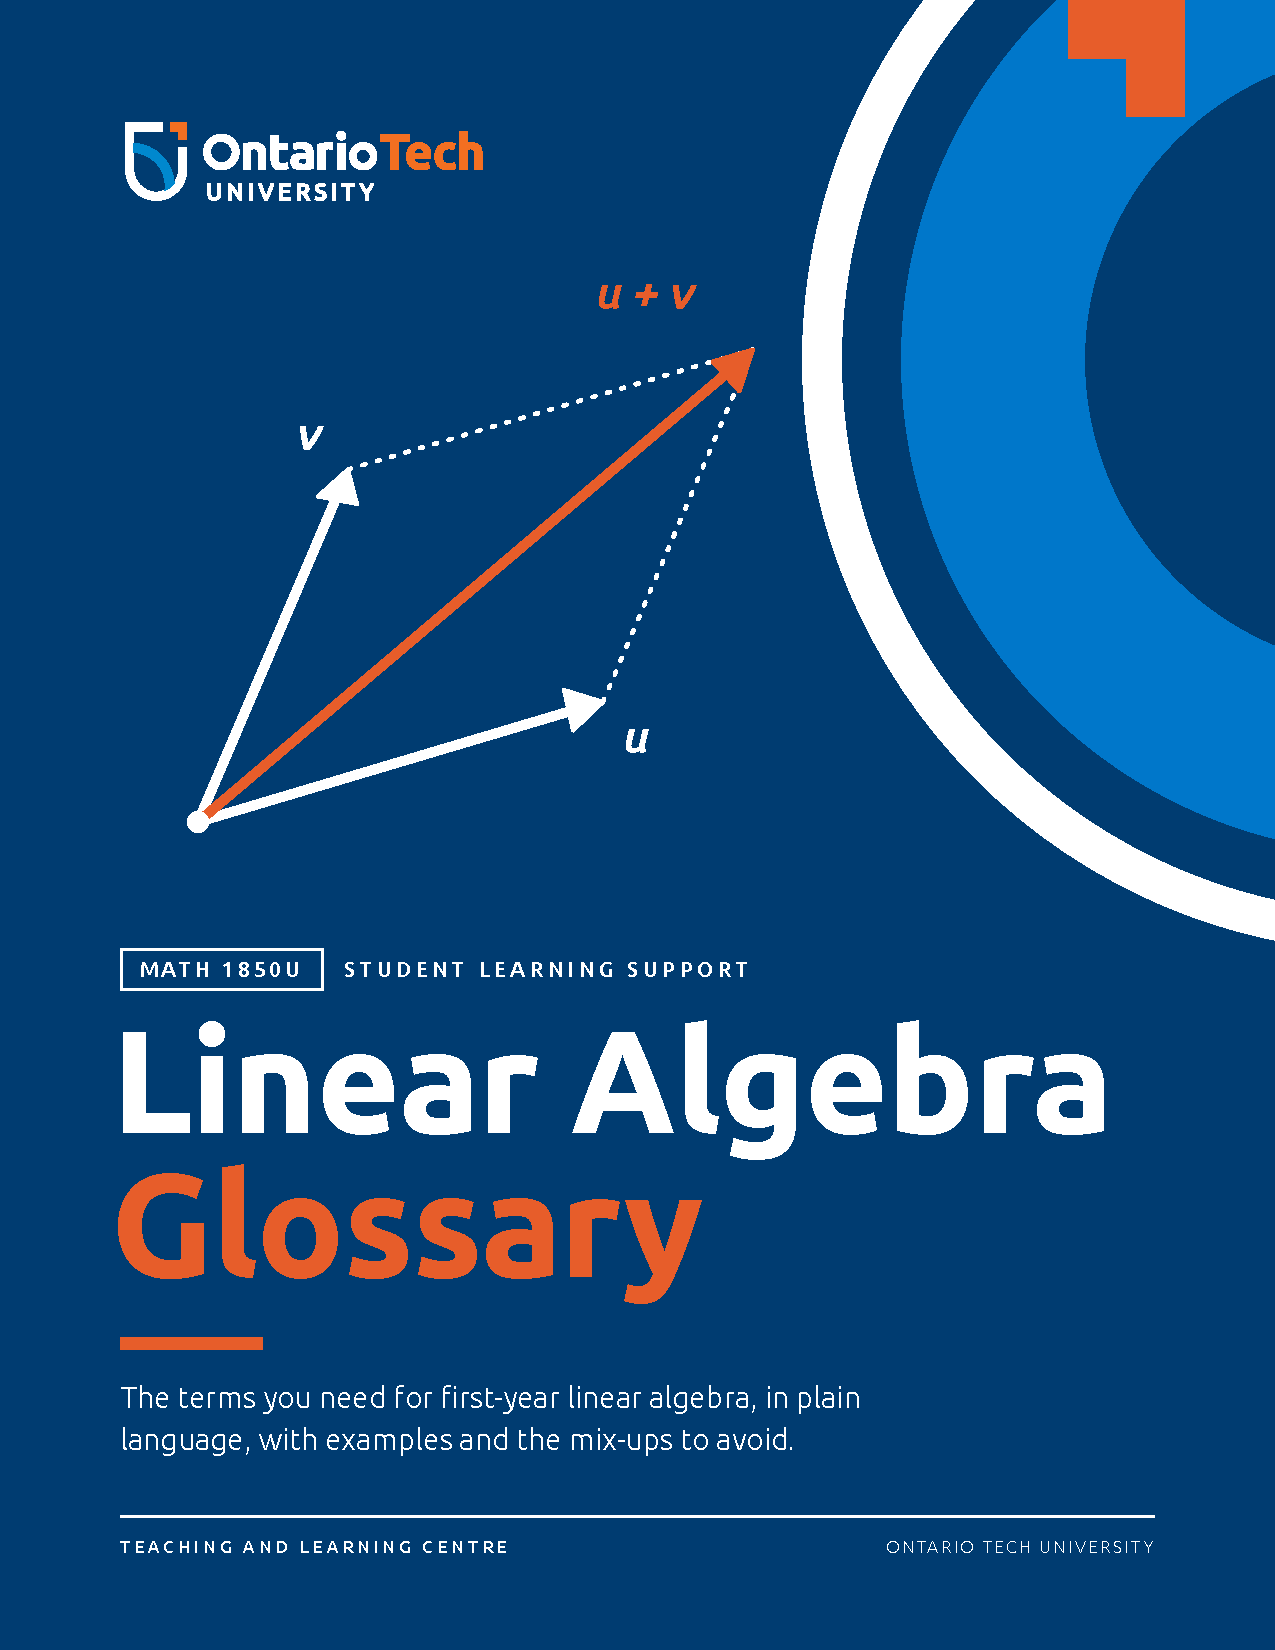
\includegraphics[width=\paperwidth,height=\paperheight]{cover/cover.pdf}};
\end{tikzpicture}
\null
\clearpage
\setcounter{nocorner}{0}

% ================================================================ CONTENTS (Simcoe Blue page)
\thispagestyle{empty}
\phantomsection\label{p:contents}
\pdfbookmark[1]{Contents}{bm:contents}
\begin{tikzpicture}[remember picture,overlay]
  \fill[SimcoeBlue] (current page.south west) rectangle (current page.north east);
  \begin{scope}
    \clip (current page.south west) rectangle (current page.north east);
    \draw[FutureBlue,line width=0.55in] ($(current page.north east)+(0.1in,-0.4in)$) circle (1.85in);
    \draw[white,line width=0.18in] ($(current page.north east)+(0.1in,-0.4in)$) circle (2.55in);
  \end{scope}
\end{tikzpicture}%
\vspace*{0.2in}
{\bfseries\fontsize{40}{44}\selectfont\color{white}Contents\par}
\vspace{16pt}
\tcbox[colback=SimcoeBlue,colframe=white,boxrule=0.6pt,arc=0pt,left=6pt,right=6pt,top=3pt,bottom=3pt]
  {\labelfont\fontsize{6.4}{8}\selectfont\color{white}\begin{tabular}{@{}l@{}}INTERACTIVE PDF\\CLICK ANY TITLE TO JUMP\end{tabular}}
\vspace{26pt}

{\color{white}\noindent\begin{minipage}[t]{2.05in}\raggedright
{\labelfont\fontsize{7.8}{9}\selectfont\color{FutureBlue}START HERE}\par\vspace{3pt}{\color{FutureBlue}\rule{\linewidth}{1pt}}\par\vspace{12pt}
\hyperref[p:howto]{\makebox[0.36in][l]{\medium\fontsize{9.5}{11}\selectfont\pageref{p:howto}}{\labelfont\fontsize{8.6}{11}\selectfont HOW TO USE THIS GLOSSARY}}\par\vspace{11pt}
\hyperref[p:notation]{\makebox[0.36in][l]{\medium\fontsize{9.5}{11}\selectfont\pageref{p:notation}}{\labelfont\fontsize{8.6}{11}\selectfont NOTATION DECODER}}\par\vspace{11pt}
\hyperref[p:pairs]{\makebox[0.36in][l]{\medium\fontsize{9.5}{11}\selectfont\pageref{p:pairs}}{\labelfont\fontsize{8.6}{11}\selectfont COMMON MIX-UPS}}\par\vspace{11pt}
\hyperref[p:index]{\makebox[0.36in][l]{\medium\fontsize{9.5}{11}\selectfont\pageref{p:index}}{\labelfont\fontsize{8.6}{11}\selectfont A-Z INDEX}}\par\vspace{11pt}
\end{minipage}\hspace{0.45in}\begin{minipage}[t]{4.2in}\raggedright
{\labelfont\fontsize{7.8}{9}\selectfont\color{FutureBlue}THE TERMS}\par\vspace{3pt}{\color{FutureBlue}\rule{\linewidth}{1pt}}\par\vspace{12pt}
\hyperref[s:systems]{\makebox[0.36in][l]{\medium\fontsize{9.5}{11}\selectfont\pageref{s:systems}}\makebox[0.34in][l]{\bfseries\fontsize{16}{11}\selectfont\color{FutureBlue}01}\parbox[t]{3.4in}{\raggedright{\labelfont\fontsize{8.6}{11}\selectfont SYSTEMS OF LINEAR EQUATIONS}\\[1pt]{\light\fontsize{8}{10}\selectfont 18 terms}}}\par\vspace{11pt}
\hyperref[s:matrices]{\makebox[0.36in][l]{\medium\fontsize{9.5}{11}\selectfont\pageref{s:matrices}}\makebox[0.34in][l]{\bfseries\fontsize{16}{11}\selectfont\color{FutureBlue}02}\parbox[t]{3.4in}{\raggedright{\labelfont\fontsize{8.6}{11}\selectfont MATRICES AND MATRIX ALGEBRA}\\[1pt]{\light\fontsize{8}{10}\selectfont 24 terms}}}\par\vspace{11pt}
\hyperref[s:special]{\makebox[0.36in][l]{\medium\fontsize{9.5}{11}\selectfont\pageref{s:special}}\makebox[0.34in][l]{\bfseries\fontsize{16}{11}\selectfont\color{FutureBlue}03}\parbox[t]{3.4in}{\raggedright{\labelfont\fontsize{8.6}{11}\selectfont SPECIAL MATRICES AND INVERTIBILITY}\\[1pt]{\light\fontsize{8}{10}\selectfont 8 terms}}}\par\vspace{11pt}
\hyperref[s:determinants]{\makebox[0.36in][l]{\medium\fontsize{9.5}{11}\selectfont\pageref{s:determinants}}\makebox[0.34in][l]{\bfseries\fontsize{16}{11}\selectfont\color{FutureBlue}04}\parbox[t]{3.4in}{\raggedright{\labelfont\fontsize{8.6}{11}\selectfont DETERMINANTS}\\[1pt]{\light\fontsize{8}{10}\selectfont 6 terms}}}\par\vspace{11pt}
\hyperref[s:vectors]{\makebox[0.36in][l]{\medium\fontsize{9.5}{11}\selectfont\pageref{s:vectors}}\makebox[0.34in][l]{\bfseries\fontsize{16}{11}\selectfont\color{FutureBlue}05}\parbox[t]{3.4in}{\raggedright{\labelfont\fontsize{8.6}{11}\selectfont VECTORS IN $\mathbb{R}^n$}\\[1pt]{\light\fontsize{8}{10}\selectfont 24 terms}}}\par\vspace{11pt}
\hyperref[s:spaces]{\makebox[0.36in][l]{\medium\fontsize{9.5}{11}\selectfont\pageref{s:spaces}}\makebox[0.34in][l]{\bfseries\fontsize{16}{11}\selectfont\color{FutureBlue}06}\parbox[t]{3.4in}{\raggedright{\labelfont\fontsize{8.6}{11}\selectfont VECTOR SPACES AND SUBSPACES}\\[1pt]{\light\fontsize{8}{10}\selectfont 10 terms}}}\par\vspace{11pt}
\hyperref[s:basis]{\makebox[0.36in][l]{\medium\fontsize{9.5}{11}\selectfont\pageref{s:basis}}\makebox[0.34in][l]{\bfseries\fontsize{16}{11}\selectfont\color{FutureBlue}07}\parbox[t]{3.4in}{\raggedright{\labelfont\fontsize{8.6}{11}\selectfont SPAN, INDEPENDENCE AND BASIS}\\[1pt]{\light\fontsize{8}{10}\selectfont 8 terms}}}\par\vspace{11pt}
\hyperref[s:dimension]{\makebox[0.36in][l]{\medium\fontsize{9.5}{11}\selectfont\pageref{s:dimension}}\makebox[0.34in][l]{\bfseries\fontsize{16}{11}\selectfont\color{FutureBlue}08}\parbox[t]{3.4in}{\raggedright{\labelfont\fontsize{8.6}{11}\selectfont DIMENSION AND THE FUNDAMENTAL SUBSPACES}\\[1pt]{\light\fontsize{8}{10}\selectfont 13 terms}}}\par\vspace{11pt}
\hyperref[s:transformations]{\makebox[0.36in][l]{\medium\fontsize{9.5}{11}\selectfont\pageref{s:transformations}}\makebox[0.34in][l]{\bfseries\fontsize{16}{11}\selectfont\color{FutureBlue}09}\parbox[t]{3.4in}{\raggedright{\labelfont\fontsize{8.6}{11}\selectfont LINEAR TRANSFORMATIONS}\\[1pt]{\light\fontsize{8}{10}\selectfont 20 terms}}}\par\vspace{11pt}
\hyperref[s:eigen]{\makebox[0.36in][l]{\medium\fontsize{9.5}{11}\selectfont\pageref{s:eigen}}\makebox[0.34in][l]{\bfseries\fontsize{16}{11}\selectfont\color{FutureBlue}10}\parbox[t]{3.4in}{\raggedright{\labelfont\fontsize{8.6}{11}\selectfont EIGENVALUES AND DIAGONALIZATION}\\[1pt]{\light\fontsize{8}{10}\selectfont 12 terms}}}\par\vspace{11pt}
\hyperref[s:inner]{\makebox[0.36in][l]{\medium\fontsize{9.5}{11}\selectfont\pageref{s:inner}}\makebox[0.34in][l]{\bfseries\fontsize{16}{11}\selectfont\color{FutureBlue}11}\parbox[t]{3.4in}{\raggedright{\labelfont\fontsize{8.6}{11}\selectfont INNER PRODUCTS AND ORTHOGONALITY}\\[1pt]{\light\fontsize{8}{10}\selectfont 15 terms}}}\par\vspace{11pt}
\end{minipage}}
\clearpage

% ================================================================ HOW TO USE
\renewcommand{\cursec}{Start here}
\pdfbookmark[1]{How to use this glossary}{bm:howto}
\phantomsection\label{p:howto}
\pagetitle{How to use this glossary}{Start here}
{\light\fontsize{11.5}{16}\selectfont\color{SpiritNavy}
Linear algebra has a lot of vocabulary, and many of the words sound alike. This glossary gives each term
from MATH 1850U in plain language first, then the precise definition, a small example, and a mistake
students often make with it.\par}

\vspace{14pt}
\lbl[SimcoeBlue]{Anatomy of an entry}\par\vspace{3pt}{\color{FutureBlue}\rule{\linewidth}{0.8pt}}\par\vspace{12pt}

% ---- annotated sample entry (not linked, not bookmarked)
\newcommand{\callout}[2]{\makebox[0pt][r]{\tikz[baseline=-0.6ex]{\fill[Tangerine] (0,0) circle (6.5pt);
  \node[white,font=\bfseries\fontsize{8}{8}\selectfont] at (0,0) {#1};}\hspace{6pt}}#2}
\noindent\begin{minipage}[t]{\leftcol}\raggedright
  {\bfseries\fontsize{12.6}{14.6}\selectfont\color{FutureBlue}\callout{1}{Span}\par}%
  \vspace{5pt}\termtag{\callout{2}{MODULE 7A}}
\end{minipage}\hfill
\begin{minipage}[t]{\dimexpr\linewidth-\leftcol-0.22in\relax}\raggedright\fontsize{9.6}{13.4}\selectfont
  \plainwords{\callout{3}{Everything you can build from a set of vectors using linear combinations.}}
  \begin{defbox}\callout{4}{\lbl[SimcoeBlue]{Definition}}\par\vspace{2pt}
    The set of all \textcolor{SimcoeBlue}{\medium linear combinations} $k_1\mathbf{v}_1 + \dots + k_r\mathbf{v}_r$
    of the vectors in $S$, written $\operatorname{span}(S)$.\end{defbox}
  \begin{exbox}\callout{5}{\lbl[DarkGrey]{Example}}\par\vspace{2pt}
    $\operatorname{span}\{(1, 0, 0), (0, 1, 0)\}$ is the $xy$-plane in $\mathbb{R}^3$.\end{exbox}
  \begin{watchbox}\callout{6}{\lbl[FutureBlue]{Don't confuse with}}\par\vspace{2pt}
    \textcolor{SimcoeBlue}{\medium Basis}. A spanning set can contain redundant vectors, while a basis cannot.\end{watchbox}
  \par\vspace{6pt}{\fontsize{8.6}{12}\selectfont\callout{7}{\lbl[DarkGrey]{See also}}\hspace{5pt}%
    \textcolor{SimcoeBlue}{\medium Spanning set, Basis, Column space}\par}
\end{minipage}

\vspace{14pt}
{\fontsize{9}{12.4}\selectfont
\begin{multicols}{2}\raggedright
\newcommand{\key}[2]{\noindent\makebox[0.3in][l]{\tikz[baseline=-0.6ex]{\fill[Tangerine] (0,0) circle (6.5pt);
  \node[white,font=\bfseries\fontsize{8}{8}\selectfont] at (0,0) {#1};}}\parbox[t]{\dimexpr\linewidth-0.3in}{#2}\par\vspace{5pt}}
\key{1}{\textbf{The term}, as it is written in the course notes.}
\key{2}{\textbf{Module} where the term is introduced. An \textbf{Application} badge marks terms that come
  from an applied example rather than the core theory.}
\key{3}{\textbf{In plain words.} Start here if the formal definition does not make sense yet.}
\key{4}{\textbf{Definition.} The precise version to use on assignments and tests.}
\key{5}{\textbf{Example.} A small, concrete case.}
\key{6}{\textbf{Don't confuse with.} A common mix-up for this term and how to tell the two apart.}
\key{7}{\textbf{See also} and \textbf{also called}. Related terms and other names you may see in other
  textbooks or videos.}
\end{multicols}}

\vspace{4pt}
\lbl[SimcoeBlue]{Finding your way around}\par\vspace{3pt}{\color{FutureBlue}\rule{\linewidth}{0.8pt}}\par\vspace{10pt}
{\fontsize{9}{12.4}\selectfont
\begin{itemize}[leftmargin=1em,itemsep=2pt]
  \item[\textcolor{Tangerine}{\rule{4pt}{4pt}}] \textbf{Everything in \textcolor{SimcoeBlue}{blue} is a link.}
    Click a term to jump to its entry.
  \item[\textcolor{Tangerine}{\rule{4pt}{4pt}}] The \textbf{footer} on every page links back to the
    \hyperref[p:contents]{\textcolor{SimcoeBlue}{\medium Contents}},
    \hyperref[p:notation]{\textcolor{SimcoeBlue}{\medium Notation decoder}},
    \hyperref[p:pairs]{\textcolor{SimcoeBlue}{\medium Common mix-ups}} and
    \hyperref[p:index]{\textcolor{SimcoeBlue}{\medium A-Z index}}.
  \item[\textcolor{Tangerine}{\rule{4pt}{4pt}}] Open your PDF viewer's \textbf{bookmarks} panel to see
    every section and term in a sidebar.
  \item[\textcolor{Tangerine}{\rule{4pt}{4pt}}] Terms are grouped in \textbf{course order}, so each section
    builds on the ones before it. Use the A-Z index if you only know the word.
\end{itemize}}

\clearpage

% ================================================================ NOTATION
\renewcommand{\cursec}{Notation decoder}
\pdfbookmark[1]{Notation decoder}{bm:notation}
\phantomsection\label{p:notation}
\pagetitle{Notation decoder}{Can't search for a symbol? Look it up here}
{\fontsize{9.2}{12.2}\selectfont
\par\ifdim\dimexpr\pagegoal-\pagetotal\relax<1.1in\relax\ifdim\pagegoal<\maxdimen\newpage\fi\fi\vspace{10pt}\lbl[SimcoeBlue]{Matrices and systems}\par\vspace{3pt}{\color{FutureBlue}\rule{\linewidth}{0.8pt}}\par\nopagebreak\vspace{2pt}
\noindent\begin{tabularx}{\linewidth}{@{}>{\raggedright\arraybackslash}p{1.45in}>{\raggedright\arraybackslash}X>{\raggedright\arraybackslash}p{1.55in}@{}}$A,\ B,\ C$ & Capital letters name matrices & \gl{matrix}{Matrix}\end{tabularx}\par\vspace{2.5pt}
\noindent\begin{tabularx}{\linewidth}{@{}>{\raggedright\arraybackslash}p{1.45in}>{\raggedright\arraybackslash}X>{\raggedright\arraybackslash}p{1.55in}@{}}$a_{ij}$, $(A)_{ij}$ & The entry in row $i$, column $j$ of $A$ & \gl{entry}{Entry}\end{tabularx}\par\vspace{2.5pt}
\noindent\begin{tabularx}{\linewidth}{@{}>{\raggedright\arraybackslash}p{1.45in}>{\raggedright\arraybackslash}X>{\raggedright\arraybackslash}p{1.55in}@{}}$m \times n$ & ``$m$ by $n$'': $m$ rows and $n$ columns & \gl{size}{Size}\end{tabularx}\par\vspace{2.5pt}
\noindent\begin{tabularx}{\linewidth}{@{}>{\raggedright\arraybackslash}p{1.45in}>{\raggedright\arraybackslash}X>{\raggedright\arraybackslash}p{1.55in}@{}}$[\,A \mid \mathbf{b}\,]$ & Augmented matrix of $A\mathbf{x} = \mathbf{b}$ & \gl{augmented-matrix}{Augmented matrix}\end{tabularx}\par\vspace{2.5pt}
\noindent\begin{tabularx}{\linewidth}{@{}>{\raggedright\arraybackslash}p{1.45in}>{\raggedright\arraybackslash}X>{\raggedright\arraybackslash}p{1.55in}@{}}$A\mathbf{x} = \mathbf{b}$ & A linear system in matrix form & \gl{matrix-form}{Matrix form}\end{tabularx}\par\vspace{2.5pt}
\noindent\begin{tabularx}{\linewidth}{@{}>{\raggedright\arraybackslash}p{1.45in}>{\raggedright\arraybackslash}X>{\raggedright\arraybackslash}p{1.55in}@{}}$R_2 \to R_2 - 3R_1$ & Row operation: replace row 2 by row 2 minus 3 times row 1 & \gl{elementary-row-operations}{Row operations}\end{tabularx}\par\vspace{2.5pt}
\noindent\begin{tabularx}{\linewidth}{@{}>{\raggedright\arraybackslash}p{1.45in}>{\raggedright\arraybackslash}X>{\raggedright\arraybackslash}p{1.55in}@{}}$I$, $I_n$ & Identity matrix of order $n$ & \gl{identity-matrix}{Identity matrix}\end{tabularx}\par\vspace{2.5pt}
\noindent\begin{tabularx}{\linewidth}{@{}>{\raggedright\arraybackslash}p{1.45in}>{\raggedright\arraybackslash}X>{\raggedright\arraybackslash}p{1.55in}@{}}$0$, $0_{m \times n}$ & Zero matrix & \gl{zero-matrix}{Zero matrix}\end{tabularx}\par\vspace{2.5pt}
\noindent\begin{tabularx}{\linewidth}{@{}>{\raggedright\arraybackslash}p{1.45in}>{\raggedright\arraybackslash}X>{\raggedright\arraybackslash}p{1.55in}@{}}$A^T$ & ``$A$ transpose'' & \gl{transpose}{Transpose}\end{tabularx}\par\vspace{2.5pt}
\noindent\begin{tabularx}{\linewidth}{@{}>{\raggedright\arraybackslash}p{1.45in}>{\raggedright\arraybackslash}X>{\raggedright\arraybackslash}p{1.55in}@{}}$A^{-1}$ & ``$A$ inverse'' (not $1/A$) & \gl{inverse}{Inverse}\end{tabularx}\par\vspace{2.5pt}
\noindent\begin{tabularx}{\linewidth}{@{}>{\raggedright\arraybackslash}p{1.45in}>{\raggedright\arraybackslash}X>{\raggedright\arraybackslash}p{1.55in}@{}}$A^k$ & $A$ multiplied by itself $k$ times & \gl{powers}{Powers of a matrix}\end{tabularx}\par\vspace{2.5pt}
\noindent\begin{tabularx}{\linewidth}{@{}>{\raggedright\arraybackslash}p{1.45in}>{\raggedright\arraybackslash}X>{\raggedright\arraybackslash}p{1.55in}@{}}$\operatorname{tr}(A)$ & Trace: the sum of the diagonal entries & \gl{trace}{Trace}\end{tabularx}\par\vspace{2.5pt}
\noindent\begin{tabularx}{\linewidth}{@{}>{\raggedright\arraybackslash}p{1.45in}>{\raggedright\arraybackslash}X>{\raggedright\arraybackslash}p{1.55in}@{}}$E$ & An elementary matrix & \gl{elementary-matrix}{Elementary matrix}\end{tabularx}\par\vspace{2.5pt}
\par\ifdim\dimexpr\pagegoal-\pagetotal\relax<1.1in\relax\ifdim\pagegoal<\maxdimen\newpage\fi\fi\vspace{10pt}\lbl[SimcoeBlue]{Determinants}\par\vspace{3pt}{\color{FutureBlue}\rule{\linewidth}{0.8pt}}\par\nopagebreak\vspace{2pt}
\noindent\begin{tabularx}{\linewidth}{@{}>{\raggedright\arraybackslash}p{1.45in}>{\raggedright\arraybackslash}X>{\raggedright\arraybackslash}p{1.55in}@{}}$\det(A)$, $|A|$ & Determinant of $A$ (can be negative) & \gl{determinant}{Determinant}\end{tabularx}\par\vspace{2.5pt}
\noindent\begin{tabularx}{\linewidth}{@{}>{\raggedright\arraybackslash}p{1.45in}>{\raggedright\arraybackslash}X>{\raggedright\arraybackslash}p{1.55in}@{}}$M_{ij}$ & Minor of entry $a_{ij}$ & \gl{minor}{Minor}\end{tabularx}\par\vspace{2.5pt}
\noindent\begin{tabularx}{\linewidth}{@{}>{\raggedright\arraybackslash}p{1.45in}>{\raggedright\arraybackslash}X>{\raggedright\arraybackslash}p{1.55in}@{}}$C_{ij}$ & Cofactor of entry $a_{ij}$, $= (-1)^{i+j}M_{ij}$ & \gl{cofactor}{Cofactor}\end{tabularx}\par\vspace{2.5pt}
\noindent\begin{tabularx}{\linewidth}{@{}>{\raggedright\arraybackslash}p{1.45in}>{\raggedright\arraybackslash}X>{\raggedright\arraybackslash}p{1.55in}@{}}$A_j$ & $A$ with column $j$ replaced by $\mathbf{b}$ & \gl{cramers-rule}{Cramer's Rule}\end{tabularx}\par\vspace{2.5pt}
\par\ifdim\dimexpr\pagegoal-\pagetotal\relax<1.1in\relax\ifdim\pagegoal<\maxdimen\newpage\fi\fi\vspace{10pt}\lbl[SimcoeBlue]{Vectors}\par\vspace{3pt}{\color{FutureBlue}\rule{\linewidth}{0.8pt}}\par\nopagebreak\vspace{2pt}
\noindent\begin{tabularx}{\linewidth}{@{}>{\raggedright\arraybackslash}p{1.45in}>{\raggedright\arraybackslash}X>{\raggedright\arraybackslash}p{1.55in}@{}}$\mathbf{u},\ \mathbf{v},\ \mathbf{w}$ & Bold lower-case letters name vectors & \gl{vector}{Vector}\end{tabularx}\par\vspace{2.5pt}
\noindent\begin{tabularx}{\linewidth}{@{}>{\raggedright\arraybackslash}p{1.45in}>{\raggedright\arraybackslash}X>{\raggedright\arraybackslash}p{1.55in}@{}}$(u_1, u_2, \dots, u_n)$ & A vector written by its components & \gl{components}{Components}\end{tabularx}\par\vspace{2.5pt}
\noindent\begin{tabularx}{\linewidth}{@{}>{\raggedright\arraybackslash}p{1.45in}>{\raggedright\arraybackslash}X>{\raggedright\arraybackslash}p{1.55in}@{}}$\overrightarrow{P_1P_2}$ & The vector from point $P_1$ to point $P_2$ & \gl{components}{Components}\end{tabularx}\par\vspace{2.5pt}
\noindent\begin{tabularx}{\linewidth}{@{}>{\raggedright\arraybackslash}p{1.45in}>{\raggedright\arraybackslash}X>{\raggedright\arraybackslash}p{1.55in}@{}}$\mathbf{u} \cdot \mathbf{v}$ & Dot product (a number) & \gl{dot-product}{Dot product}\end{tabularx}\par\vspace{2.5pt}
\noindent\begin{tabularx}{\linewidth}{@{}>{\raggedright\arraybackslash}p{1.45in}>{\raggedright\arraybackslash}X>{\raggedright\arraybackslash}p{1.55in}@{}}$\mathbf{u} \times \mathbf{v}$ & Cross product (a vector, $\mathbb{R}^3$ only) & \gl{cross-product}{Cross product}\end{tabularx}\par\vspace{2.5pt}
\noindent\begin{tabularx}{\linewidth}{@{}>{\raggedright\arraybackslash}p{1.45in}>{\raggedright\arraybackslash}X>{\raggedright\arraybackslash}p{1.55in}@{}}$\|\mathbf{v}\|$ & Norm (length) of $\mathbf{v}$ & \gl{norm}{Norm}\end{tabularx}\par\vspace{2.5pt}
\noindent\begin{tabularx}{\linewidth}{@{}>{\raggedright\arraybackslash}p{1.45in}>{\raggedright\arraybackslash}X>{\raggedright\arraybackslash}p{1.55in}@{}}$d(\mathbf{u}, \mathbf{v})$ & Distance between $\mathbf{u}$ and $\mathbf{v}$ & \gl{euclidean-distance}{Euclidean distance}\end{tabularx}\par\vspace{2.5pt}
\noindent\begin{tabularx}{\linewidth}{@{}>{\raggedright\arraybackslash}p{1.45in}>{\raggedright\arraybackslash}X>{\raggedright\arraybackslash}p{1.55in}@{}}$\mathbf{e}_i$;\ $\mathbf{i},\ \mathbf{j},\ \mathbf{k}$ & Standard unit vectors & \gl{standard-unit-vectors}{Standard unit vectors}\end{tabularx}\par\vspace{2.5pt}
\noindent\begin{tabularx}{\linewidth}{@{}>{\raggedright\arraybackslash}p{1.45in}>{\raggedright\arraybackslash}X>{\raggedright\arraybackslash}p{1.55in}@{}}$\theta$ & Angle between two vectors, $0 \leq \theta \leq \pi$ & \gl{angle-between}{Angle between vectors}\end{tabularx}\par\vspace{2.5pt}
\noindent\begin{tabularx}{\linewidth}{@{}>{\raggedright\arraybackslash}p{1.45in}>{\raggedright\arraybackslash}X>{\raggedright\arraybackslash}p{1.55in}@{}}$\operatorname{proj}_{\mathbf{a}}\mathbf{u}$ & Projection of $\mathbf{u}$ onto $\mathbf{a}$ & \gl{projection-onto-vector}{Projection onto a vector}\end{tabularx}\par\vspace{2.5pt}
\noindent\begin{tabularx}{\linewidth}{@{}>{\raggedright\arraybackslash}p{1.45in}>{\raggedright\arraybackslash}X>{\raggedright\arraybackslash}p{1.55in}@{}}$\mathbf{n}$ & A normal vector to a plane & \gl{normal-vector}{Normal vector}\end{tabularx}\par\vspace{2.5pt}
\par\ifdim\dimexpr\pagegoal-\pagetotal\relax<1.1in\relax\ifdim\pagegoal<\maxdimen\newpage\fi\fi\vspace{10pt}\lbl[SimcoeBlue]{Vector spaces and subspaces}\par\vspace{3pt}{\color{FutureBlue}\rule{\linewidth}{0.8pt}}\par\nopagebreak\vspace{2pt}
\noindent\begin{tabularx}{\linewidth}{@{}>{\raggedright\arraybackslash}p{1.45in}>{\raggedright\arraybackslash}X>{\raggedright\arraybackslash}p{1.55in}@{}}$\mathbb{R}^n$ & $n$-space: all vectors with $n$ real components & \gl{n-space}{$n$-space}\end{tabularx}\par\vspace{2.5pt}
\noindent\begin{tabularx}{\linewidth}{@{}>{\raggedright\arraybackslash}p{1.45in}>{\raggedright\arraybackslash}X>{\raggedright\arraybackslash}p{1.55in}@{}}$V,\ W$ & A vector space and (often) a subspace of it & \gl{vector-space}{Vector space}\end{tabularx}\par\vspace{2.5pt}
\noindent\begin{tabularx}{\linewidth}{@{}>{\raggedright\arraybackslash}p{1.45in}>{\raggedright\arraybackslash}X>{\raggedright\arraybackslash}p{1.55in}@{}}$\mathbf{0}$;\ $\{\mathbf{0}\}$ & Zero vector;\ zero vector space & \gl{zero-vector}{Zero vector}\end{tabularx}\par\vspace{2.5pt}
\noindent\begin{tabularx}{\linewidth}{@{}>{\raggedright\arraybackslash}p{1.45in}>{\raggedright\arraybackslash}X>{\raggedright\arraybackslash}p{1.55in}@{}}$P_n$ & Polynomials of degree at most $n$ & \gl{polynomial-space}{$P_n$}\end{tabularx}\par\vspace{2.5pt}
\noindent\begin{tabularx}{\linewidth}{@{}>{\raggedright\arraybackslash}p{1.45in}>{\raggedright\arraybackslash}X>{\raggedright\arraybackslash}p{1.55in}@{}}$M_{mn}$ & All $m \times n$ matrices & \gl{matrix-space}{$M_{mn}$}\end{tabularx}\par\vspace{2.5pt}
\noindent\begin{tabularx}{\linewidth}{@{}>{\raggedright\arraybackslash}p{1.45in}>{\raggedright\arraybackslash}X>{\raggedright\arraybackslash}p{1.55in}@{}}$F(-\infty, \infty)$ & All real-valued functions on $\mathbb{R}$ & \gl{function-space}{Function space}\end{tabularx}\par\vspace{2.5pt}
\noindent\begin{tabularx}{\linewidth}{@{}>{\raggedright\arraybackslash}p{1.45in}>{\raggedright\arraybackslash}X>{\raggedright\arraybackslash}p{1.55in}@{}}$C[a, b]$ & Continuous functions on $[a, b]$ & \gl{continuous-functions}{$C[a, b]$}\end{tabularx}\par\vspace{2.5pt}
\noindent\begin{tabularx}{\linewidth}{@{}>{\raggedright\arraybackslash}p{1.45in}>{\raggedright\arraybackslash}X>{\raggedright\arraybackslash}p{1.55in}@{}}$\operatorname{span}(S)$ & All linear combinations of the vectors in $S$ & \gl{span}{Span}\end{tabularx}\par\vspace{2.5pt}
\noindent\begin{tabularx}{\linewidth}{@{}>{\raggedright\arraybackslash}p{1.45in}>{\raggedright\arraybackslash}X>{\raggedright\arraybackslash}p{1.55in}@{}}$(\mathbf{v})_S$ & Coordinate vector of $\mathbf{v}$ relative to basis $S$ & \gl{coordinate-vector}{Coordinate vector}\end{tabularx}\par\vspace{2.5pt}
\noindent\begin{tabularx}{\linewidth}{@{}>{\raggedright\arraybackslash}p{1.45in}>{\raggedright\arraybackslash}X>{\raggedright\arraybackslash}p{1.55in}@{}}$\dim(V)$ & Dimension of $V$ & \gl{dimension}{Dimension}\end{tabularx}\par\vspace{2.5pt}
\noindent\begin{tabularx}{\linewidth}{@{}>{\raggedright\arraybackslash}p{1.45in}>{\raggedright\arraybackslash}X>{\raggedright\arraybackslash}p{1.55in}@{}}$\operatorname{rank}(A)$ & Rank of $A$ & \gl{rank}{Rank}\end{tabularx}\par\vspace{2.5pt}
\noindent\begin{tabularx}{\linewidth}{@{}>{\raggedright\arraybackslash}p{1.45in}>{\raggedright\arraybackslash}X>{\raggedright\arraybackslash}p{1.55in}@{}}$\operatorname{nullity}(A)$ & Nullity of $A$ & \gl{nullity}{Nullity}\end{tabularx}\par\vspace{2.5pt}
\noindent\begin{tabularx}{\linewidth}{@{}>{\raggedright\arraybackslash}p{1.45in}>{\raggedright\arraybackslash}X>{\raggedright\arraybackslash}p{1.55in}@{}}$W^{\perp}$ & ``$W$ perp'': the orthogonal complement of $W$ & \gl{orthogonal-complement}{Orthogonal complement}\end{tabularx}\par\vspace{2.5pt}
\par\ifdim\dimexpr\pagegoal-\pagetotal\relax<1.1in\relax\ifdim\pagegoal<\maxdimen\newpage\fi\fi\vspace{10pt}\lbl[SimcoeBlue]{Transformations}\par\vspace{3pt}{\color{FutureBlue}\rule{\linewidth}{0.8pt}}\par\nopagebreak\vspace{2pt}
\noindent\begin{tabularx}{\linewidth}{@{}>{\raggedright\arraybackslash}p{1.45in}>{\raggedright\arraybackslash}X>{\raggedright\arraybackslash}p{1.55in}@{}}$T\colon V \to W$ & $T$ maps $V$ (domain) to $W$ (codomain) & \gl{transformation}{Transformation}\end{tabularx}\par\vspace{2.5pt}
\noindent\begin{tabularx}{\linewidth}{@{}>{\raggedright\arraybackslash}p{1.45in}>{\raggedright\arraybackslash}X>{\raggedright\arraybackslash}p{1.55in}@{}}$T_A$ & Multiplication by $A$:\ $T_A(\mathbf{x}) = A\mathbf{x}$ & \gl{matrix-transformation}{Matrix transformation}\end{tabularx}\par\vspace{2.5pt}
\noindent\begin{tabularx}{\linewidth}{@{}>{\raggedright\arraybackslash}p{1.45in}>{\raggedright\arraybackslash}X>{\raggedright\arraybackslash}p{1.55in}@{}}$[T]$ & Standard matrix of $T$ & \gl{standard-matrix}{Standard matrix}\end{tabularx}\par\vspace{2.5pt}
\noindent\begin{tabularx}{\linewidth}{@{}>{\raggedright\arraybackslash}p{1.45in}>{\raggedright\arraybackslash}X>{\raggedright\arraybackslash}p{1.55in}@{}}$T_B \circ T_A$ & Do $T_A$ first, then $T_B$ & \gl{composition}{Composition}\end{tabularx}\par\vspace{2.5pt}
\noindent\begin{tabularx}{\linewidth}{@{}>{\raggedright\arraybackslash}p{1.45in}>{\raggedright\arraybackslash}X>{\raggedright\arraybackslash}p{1.55in}@{}}$\ker(T_A)$ & Kernel of $T_A$ (the nullspace of $A$) & \gl{kernel}{Kernel}\end{tabularx}\par\vspace{2.5pt}
\noindent\begin{tabularx}{\linewidth}{@{}>{\raggedright\arraybackslash}p{1.45in}>{\raggedright\arraybackslash}X>{\raggedright\arraybackslash}p{1.55in}@{}}$R(T_A)$ & Range of $T_A$ (the column space of $A$) & \gl{range}{Range}\end{tabularx}\par\vspace{2.5pt}
\noindent\begin{tabularx}{\linewidth}{@{}>{\raggedright\arraybackslash}p{1.45in}>{\raggedright\arraybackslash}X>{\raggedright\arraybackslash}p{1.55in}@{}}$T^{-1}$ & Inverse transformation & \gl{inverse-transformation}{Inverse transformation}\end{tabularx}\par\vspace{2.5pt}
\par\ifdim\dimexpr\pagegoal-\pagetotal\relax<1.1in\relax\ifdim\pagegoal<\maxdimen\newpage\fi\fi\vspace{10pt}\lbl[SimcoeBlue]{Eigenvalues and inner products}\par\vspace{3pt}{\color{FutureBlue}\rule{\linewidth}{0.8pt}}\par\nopagebreak\vspace{2pt}
\noindent\begin{tabularx}{\linewidth}{@{}>{\raggedright\arraybackslash}p{1.45in}>{\raggedright\arraybackslash}X>{\raggedright\arraybackslash}p{1.55in}@{}}$\lambda$ & ``lambda'': an eigenvalue & \gl{eigenvalue}{Eigenvalue}\end{tabularx}\par\vspace{2.5pt}
\noindent\begin{tabularx}{\linewidth}{@{}>{\raggedright\arraybackslash}p{1.45in}>{\raggedright\arraybackslash}X>{\raggedright\arraybackslash}p{1.55in}@{}}$\det(A - \lambda I) = 0$ & Characteristic equation & \gl{characteristic-equation}{Characteristic equation}\end{tabularx}\par\vspace{2.5pt}
\noindent\begin{tabularx}{\linewidth}{@{}>{\raggedright\arraybackslash}p{1.45in}>{\raggedright\arraybackslash}X>{\raggedright\arraybackslash}p{1.55in}@{}}$P^{-1}AP = D$ & $P$ diagonalizes $A$;\ $D$ is diagonal & \gl{diagonalizable}{Diagonalizable}\end{tabularx}\par\vspace{2.5pt}
\noindent\begin{tabularx}{\linewidth}{@{}>{\raggedright\arraybackslash}p{1.45in}>{\raggedright\arraybackslash}X>{\raggedright\arraybackslash}p{1.55in}@{}}$\langle \mathbf{u}, \mathbf{v} \rangle$ & Inner product of $\mathbf{u}$ and $\mathbf{v}$ & \gl{inner-product}{Inner product}\end{tabularx}\par\vspace{2.5pt}
\noindent\begin{tabularx}{\linewidth}{@{}>{\raggedright\arraybackslash}p{1.45in}>{\raggedright\arraybackslash}X>{\raggedright\arraybackslash}p{1.55in}@{}}$\operatorname{proj}_W\mathbf{u}$ & Orthogonal projection of $\mathbf{u}$ on subspace $W$ & \gl{projection-onto-subspace}{Projection onto a subspace}\end{tabularx}\par\vspace{2.5pt}
\noindent\begin{tabularx}{\linewidth}{@{}>{\raggedright\arraybackslash}p{1.45in}>{\raggedright\arraybackslash}X>{\raggedright\arraybackslash}p{1.55in}@{}}$\operatorname{proj}_{W^{\perp}}\mathbf{u}$ & Component of $\mathbf{u}$ orthogonal to $W$ & \gl{component-orthogonal-w}{Component orthogonal to $W$}\end{tabularx}\par\vspace{2.5pt}
}
\clearpage

% ================================================================ MIX-UPS
\renewcommand{\cursec}{Common mix-ups}
\pdfbookmark[1]{Common mix-ups}{bm:pairs}
\phantomsection\label{p:pairs}
\pagetitle{Common mix-ups}{Pairs that are easy to confuse}
\begin{multicols}{2}\raggedcolumns
\begin{tcolorbox}[enhanced,breakable=false,colback=white,colframe=white,boxrule=0pt,arc=0pt,
 left=8pt,right=4pt,top=1pt,bottom=2pt,borderline west={3pt}{0pt}{SimcoeBlue},before skip=0pt,after skip=9pt]
{\bfseries\fontsize{10.8}{13}\selectfont\glw{span}{\textcolor{FutureBlue}{Span}}\ {\color{Tangerine}\medium vs.}\ \glw{basis}{\textcolor{FutureBlue}{Basis}}\par}
\vspace{3pt}{\fontsize{8.8}{12}\selectfont A span is \emph{everything} you can build from some vectors. A basis is a set of vectors that builds everything with nothing redundant. Every basis spans its space, but a spanning set might not be a basis.\par}
\end{tcolorbox}
\begin{tcolorbox}[enhanced,breakable=false,colback=white,colframe=white,boxrule=0pt,arc=0pt,
 left=8pt,right=4pt,top=1pt,bottom=2pt,borderline west={3pt}{0pt}{SimcoeBlue},before skip=0pt,after skip=9pt]
{\bfseries\fontsize{10.8}{13}\selectfont\glw{nullspace}{\textcolor{FutureBlue}{Nullspace}}\ {\color{Tangerine}\medium vs.}\ \glw{column-space}{\textcolor{FutureBlue}{Column space}}\par}
\vspace{3pt}{\fontsize{8.8}{12}\selectfont The nullspace is the set of inputs $\mathbf{x}$ with $A\mathbf{x} = \mathbf{0}$, and it lives in $\mathbb{R}^n$. The column space is the set of outputs $A\mathbf{x}$, and it lives in $\mathbb{R}^m$.\par}
\end{tcolorbox}
\begin{tcolorbox}[enhanced,breakable=false,colback=white,colframe=white,boxrule=0pt,arc=0pt,
 left=8pt,right=4pt,top=1pt,bottom=2pt,borderline west={3pt}{0pt}{SimcoeBlue},before skip=0pt,after skip=9pt]
{\bfseries\fontsize{10.8}{13}\selectfont\glw{rank}{\textcolor{FutureBlue}{Rank}}\ {\color{Tangerine}\medium vs.}\ \glw{nullity}{\textcolor{FutureBlue}{Nullity}}\par}
\vspace{3pt}{\fontsize{8.8}{12}\selectfont Rank counts leading 1s (leading variables). Nullity counts free variables. Together they equal the number of columns.\par}
\end{tcolorbox}
\begin{tcolorbox}[enhanced,breakable=false,colback=white,colframe=white,boxrule=0pt,arc=0pt,
 left=8pt,right=4pt,top=1pt,bottom=2pt,borderline west={3pt}{0pt}{SimcoeBlue},before skip=0pt,after skip=9pt]
{\bfseries\fontsize{10.8}{13}\selectfont\glw{eigenvalue}{\textcolor{FutureBlue}{Eigenvalue}}\ {\color{Tangerine}\medium vs.}\ \glw{eigenvector}{\textcolor{FutureBlue}{Eigenvector}}\par}
\vspace{3pt}{\fontsize{8.8}{12}\selectfont In $A\mathbf{x} = \lambda\mathbf{x}$, the number $\lambda$ is the eigenvalue and the nonzero vector $\mathbf{x}$ is the eigenvector. $0$ can be an eigenvalue, but $\mathbf{0}$ is never an eigenvector.\par}
\end{tcolorbox}
\begin{tcolorbox}[enhanced,breakable=false,colback=white,colframe=white,boxrule=0pt,arc=0pt,
 left=8pt,right=4pt,top=1pt,bottom=2pt,borderline west={3pt}{0pt}{SimcoeBlue},before skip=0pt,after skip=9pt]
{\bfseries\fontsize{10.8}{13}\selectfont\glw{algebraic-multiplicity}{\textcolor{FutureBlue}{Algebraic multiplicity}}\ {\color{Tangerine}\medium vs.}\ \glw{geometric-multiplicity}{\textcolor{FutureBlue}{Geometric multiplicity}}\par}
\vspace{3pt}{\fontsize{8.8}{12}\selectfont Algebraic multiplicity is the power of the factor in the characteristic polynomial. Geometric multiplicity is the dimension of the eigenspace. A matrix is diagonalizable exactly when they match for every eigenvalue.\par}
\end{tcolorbox}
\begin{tcolorbox}[enhanced,breakable=false,colback=white,colframe=white,boxrule=0pt,arc=0pt,
 left=8pt,right=4pt,top=1pt,bottom=2pt,borderline west={3pt}{0pt}{SimcoeBlue},before skip=0pt,after skip=9pt]
{\bfseries\fontsize{10.8}{13}\selectfont\glw{diagonal-matrix}{\textcolor{FutureBlue}{Diagonal matrix}}\ {\color{Tangerine}\medium vs.}\ \glw{diagonalizable}{\textcolor{FutureBlue}{Diagonalizable}}\par}
\vspace{3pt}{\fontsize{8.8}{12}\selectfont A diagonal matrix already has zeros off the diagonal. A diagonalizable matrix can be \emph{turned into} one by $P^{-1}AP$, but usually is not diagonal itself.\par}
\end{tcolorbox}
\begin{tcolorbox}[enhanced,breakable=false,colback=white,colframe=white,boxrule=0pt,arc=0pt,
 left=8pt,right=4pt,top=1pt,bottom=2pt,borderline west={3pt}{0pt}{SimcoeBlue},before skip=0pt,after skip=9pt]
{\bfseries\fontsize{10.8}{13}\selectfont\glw{dot-product}{\textcolor{FutureBlue}{Dot product}}\ {\color{Tangerine}\medium vs.}\ \glw{cross-product}{\textcolor{FutureBlue}{Cross product}}\par}
\vspace{3pt}{\fontsize{8.8}{12}\selectfont $\mathbf{u} \cdot \mathbf{v}$ is a number, works in any $\mathbb{R}^n$, and is $0$ for orthogonal vectors. $\mathbf{u} \times \mathbf{v}$ is a vector, works only in $\mathbb{R}^3$, and is $\mathbf{0}$ for parallel vectors.\par}
\end{tcolorbox}
\begin{tcolorbox}[enhanced,breakable=false,colback=white,colframe=white,boxrule=0pt,arc=0pt,
 left=8pt,right=4pt,top=1pt,bottom=2pt,borderline west={3pt}{0pt}{SimcoeBlue},before skip=0pt,after skip=9pt]
{\bfseries\fontsize{10.8}{13}\selectfont\glw{minor}{\textcolor{FutureBlue}{Minor}}\ {\color{Tangerine}\medium vs.}\ \glw{cofactor}{\textcolor{FutureBlue}{Cofactor}}\par}
\vspace{3pt}{\fontsize{8.8}{12}\selectfont A minor is a smaller determinant. A cofactor is that minor with a checkerboard sign attached: $C_{ij} = (-1)^{i+j}M_{ij}$.\par}
\end{tcolorbox}
\begin{tcolorbox}[enhanced,breakable=false,colback=white,colframe=white,boxrule=0pt,arc=0pt,
 left=8pt,right=4pt,top=1pt,bottom=2pt,borderline west={3pt}{0pt}{SimcoeBlue},before skip=0pt,after skip=9pt]
{\bfseries\fontsize{10.8}{13}\selectfont\glw{codomain}{\textcolor{FutureBlue}{Codomain}}\ {\color{Tangerine}\medium vs.}\ \glw{range}{\textcolor{FutureBlue}{Range}}\par}
\vspace{3pt}{\fontsize{8.8}{12}\selectfont The codomain is where outputs are \emph{allowed} to land. The range is where they \emph{actually} land. For $T_A$, the range is the column space of $A$.\par}
\end{tcolorbox}
\begin{tcolorbox}[enhanced,breakable=false,colback=white,colframe=white,boxrule=0pt,arc=0pt,
 left=8pt,right=4pt,top=1pt,bottom=2pt,borderline west={3pt}{0pt}{SimcoeBlue},before skip=0pt,after skip=9pt]
{\bfseries\fontsize{10.8}{13}\selectfont\glw{orthogonal-set}{\textcolor{FutureBlue}{Orthogonal set}}\ {\color{Tangerine}\medium vs.}\ \glw{orthonormal}{\textcolor{FutureBlue}{Orthonormal set}}\par}
\vspace{3pt}{\fontsize{8.8}{12}\selectfont In an orthogonal set, every pair is perpendicular. An orthonormal set is the same, plus every vector has length 1. Normalize each vector to get from one to the other.\par}
\end{tcolorbox}
\begin{tcolorbox}[enhanced,breakable=false,colback=white,colframe=white,boxrule=0pt,arc=0pt,
 left=8pt,right=4pt,top=1pt,bottom=2pt,borderline west={3pt}{0pt}{SimcoeBlue},before skip=0pt,after skip=9pt]
{\bfseries\fontsize{10.8}{13}\selectfont\glw{augmented-matrix}{\textcolor{FutureBlue}{Augmented matrix}}\ {\color{Tangerine}\medium vs.}\ \glw{coefficient-matrix}{\textcolor{FutureBlue}{Coefficient matrix}}\par}
\vspace{3pt}{\fontsize{8.8}{12}\selectfont The coefficient matrix $A$ holds only the coefficients. The augmented matrix $[\,A \mid \mathbf{b}\,]$ adds the column of constants, and it is the one you row reduce to solve a system.\par}
\end{tcolorbox}
\begin{tcolorbox}[enhanced,breakable=false,colback=white,colframe=white,boxrule=0pt,arc=0pt,
 left=8pt,right=4pt,top=1pt,bottom=2pt,borderline west={3pt}{0pt}{SimcoeBlue},before skip=0pt,after skip=9pt]
{\bfseries\fontsize{10.8}{13}\selectfont\glw{kernel}{\textcolor{FutureBlue}{Kernel}}\ {\color{Tangerine}\medium vs.}\ \glw{nullspace}{\textcolor{FutureBlue}{Nullspace}}\par}
\vspace{3pt}{\fontsize{8.8}{12}\selectfont These are \emph{the same set} under two names. Use ``kernel'' when talking about a transformation $T_A$, and ``nullspace'' when talking about the matrix $A$.\par}
\end{tcolorbox}
\begin{tcolorbox}[enhanced,breakable=false,colback=white,colframe=white,boxrule=0pt,arc=0pt,
 left=8pt,right=4pt,top=1pt,bottom=2pt,borderline west={3pt}{0pt}{SimcoeBlue},before skip=0pt,after skip=9pt]
{\bfseries\fontsize{10.8}{13}\selectfont\glw{projection-onto-vector}{\textcolor{FutureBlue}{Orthogonal projection onto a vector}}\ {\color{Tangerine}\medium vs.}\ \glw{projection-onto-subspace}{\textcolor{FutureBlue}{Orthogonal projection onto a subspace}}\par}
\vspace{3pt}{\fontsize{8.8}{12}\selectfont The same idea at two scales. $\operatorname{proj}_{\mathbf{a}}\mathbf{u}$ projects onto a line. $\operatorname{proj}_W\mathbf{u}$ projects onto a whole subspace, and its formula needs an orthogonal basis for $W$.\par}
\end{tcolorbox}
\begin{tcolorbox}[enhanced,breakable=false,colback=white,colframe=white,boxrule=0pt,arc=0pt,
 left=8pt,right=4pt,top=1pt,bottom=2pt,borderline west={3pt}{0pt}{SimcoeBlue},before skip=0pt,after skip=9pt]
{\bfseries\fontsize{10.8}{13}\selectfont\glw{gaussian-elimination}{\textcolor{FutureBlue}{Gaussian elimination}}\ {\color{Tangerine}\medium vs.}\ \glw{gauss-jordan}{\textcolor{FutureBlue}{Gauss–Jordan elimination}}\par}
\vspace{3pt}{\fontsize{8.8}{12}\selectfont Gaussian elimination stops at REF and finishes with back substitution. Gauss–Jordan elimination continues to RREF and reads the answer directly.\par}
\end{tcolorbox}
\end{multicols}

% ================================================================ ENTRIES
\glsection{01}{systems}{Systems of Linear Equations}{MODULES 1A AND 1B}{Every later module builds on these words. They describe equations, their solutions, and the row reduction you will use for the rest of the course.}{18}{\glw{linear-equation}{\textcolor{FutureBlue}{Linear equation}}\par \glw{coefficient}{\textcolor{FutureBlue}{Coefficient}}\par \glw{unknown}{\textcolor{FutureBlue}{Unknown}}\par \glw{solution}{\textcolor{FutureBlue}{Solution}}\par \glw{solution-set}{\textcolor{FutureBlue}{Solution set}}\par \glw{system}{\textcolor{FutureBlue}{System of linear equations}}\par \glw{consistent}{\textcolor{FutureBlue}{Consistent / inconsistent}}\par \glw{augmented-matrix}{\textcolor{FutureBlue}{Augmented matrix}}\par \glw{elementary-row-operations}{\textcolor{FutureBlue}{Elementary row operations}}\par \glw{row-equivalent}{\textcolor{FutureBlue}{Row equivalent}}\par \glw{back-substitution}{\textcolor{FutureBlue}{Back substitution}}\par \glw{ref}{\textcolor{FutureBlue}{Row echelon form (REF)}}\par \glw{rref}{\textcolor{FutureBlue}{Reduced row echelon form (RREF)}}\par \glw{leading-one}{\textcolor{FutureBlue}{Leading 1}}\par \glw{leading-variable}{\textcolor{FutureBlue}{Leading variable / free variable}}\par \glw{parameter}{\textcolor{FutureBlue}{Parameter}}\par \glw{gaussian-elimination}{\textcolor{FutureBlue}{Gaussian elimination}}\par \glw{gauss-jordan}{\textcolor{FutureBlue}{Gauss–Jordan elimination}}\par }
\begin{glentry}{linear-equation}{Linear equation}{Linear equation}{1a}{0}
\plainwords{An equation where each variable appears on its own, to the first power, multiplied only by a number.}
\definition{A linear equation in the $n$ variables $x_1, x_2, \dots, x_n$ is an equation that can be written as $a_1x_1 + a_2x_2 + \dots + a_nx_n = b$, where $a_1, \dots, a_n$ and $b$ are real constants. If it cannot be written in this form, it is a \textbf{nonlinear equation}.}
\example{$3x_1 - 2x_2 + x_3 = 7$ is linear. $x_1x_2 = 4$, $x_1^2 + x_2 = 1$ and $\sin x_1 = 0$ are nonlinear.}
\watch{A \emph{linear} equation is not the same as the equation of a line. In three or more variables, a linear equation describes a plane or a higher-dimensional flat object.}
\entryfoot{}{\gl{coefficient}{Coefficient}, \gl{system}{System of linear equations}}
\end{glentry}

\begin{glentry}{coefficient}{Coefficient}{Coefficient}{1a}{0}
\plainwords{The number multiplying a variable.}
\definition{In $a_1x_1 + a_2x_2 + \dots + a_nx_n = b$, the constants $a_i$ are the coefficients. The word is reused later for the scalars in a \gl{linear-combination}{linear combination}.}
\example{In $4x - y + 0z = 2$, the coefficients are $4$, $-1$ and $0$.}
\entryfoot{}{\gl{linear-equation}{Linear equation}, \gl{coefficient-matrix}{Coefficient matrix}}
\end{glentry}

\begin{glentry}{unknown}{Unknown}{Unknown}{1a}{0}
\plainwords{Another name for a variable you are solving for.}
\definition{The variables $x_1, x_2, \dots, x_n$ in a linear equation or system are sometimes called the unknowns.}
\entryfoot{variable}{\gl{linear-equation}{Linear equation}, \gl{system}{System of linear equations}}
\end{glentry}

\begin{glentry}{solution}{Solution}{Solution}{1a}{0}
\plainwords{A list of values that makes every equation true at the same time.}
\definition{A solution of $a_1x_1 + \dots + a_nx_n = b$ is a sequence of $n$ numbers $s_1, \dots, s_n$ such that the equation is satisfied when $x_1 = s_1, \dots, x_n = s_n$. A solution of a \gl{system}{system} must satisfy every equation in it.}
\example{$(x, y) = (2, 1)$ is a solution of $x + y = 3$ and $x - y = 1$.}
\entryfoot{}{\gl{solution-set}{Solution set}, \gl{consistent}{Consistent / inconsistent}}
\end{glentry}

\begin{glentry}{solution-set}{Solution set}{Solution set}{1a}{0}
\plainwords{The collection of all solutions, not just one of them.}
\definition{The set of all solutions of an equation or system is called its solution set. A solution set written with \gl{parameter}{parameters} is often called the \gl{general-solution}{general solution}.}
\example{The solution set of $x + y = 3$ is $\{(3 - t,\ t) : t \in \mathbb{R}\}$, a whole line of points.}
\entryfoot{}{\gl{solution}{Solution}, \gl{general-solution}{General solution}}
\end{glentry}

\begin{glentry}{system}{System of linear equations}{System of linear equations}{1a}{0}
\plainwords{Several linear equations that must all hold at once.}
\definition{A finite set of linear equations in the variables $x_1, \dots, x_n$ is called a system of linear equations (or a linear system). A system of $m$ equations in $n$ unknowns can be written compactly as $A\mathbf{x} = \mathbf{b}$.}
\example{$\begin{aligned} x + 2y &= 5 \\ 3x - y &= 1 \end{aligned}$ is a system of 2 equations in 2 unknowns.}
\entryfoot{linear system}{\gl{consistent}{Consistent / inconsistent}, \gl{augmented-matrix}{Augmented matrix}, \gl{matrix-form}{Matrix form $A\mathbf{x} = \mathbf{b}$}}
\end{glentry}

\begin{glentry}{consistent}{Consistent / inconsistent}{Consistent / inconsistent}{1a}{0}
\plainwords{Consistent means the system has at least one solution. Inconsistent means it has none.}
\definition{A system with at least one solution is \textbf{consistent}. A system with no solutions is \textbf{inconsistent}. Every linear system has either no solutions, exactly one solution, or infinitely many solutions.}
\example{$x + y = 1$ and $x + y = 4$ is inconsistent: two parallel lines never meet. Row reduction shows this as a row $[\,0\ \ 0 \mid c\,]$ with $c \neq 0$.}
\watch{Consistent does not mean exactly one solution. A system with infinitely many solutions is still consistent.}
\entryfoot{}{\gl{solution-set}{Solution set}, \gl{rref}{Reduced row echelon form (RREF)}, \gl{homogeneous}{Homogeneous system}}
\end{glentry}

\begin{glentry}{augmented-matrix}{Augmented matrix}{Augmented matrix}{1a}{0}
\plainwords{The system's numbers written in a grid, with the right-hand sides tacked on as a last column.}
\definition{For a system $A\mathbf{x} = \mathbf{b}$, the augmented matrix is $[\,A \mid \mathbf{b}\,]$: the \gl{coefficient-matrix}{coefficient matrix} with the column of constants attached on the right.}
\example{$\begin{aligned} x + 2y &= 5 \\ 3x - y &= 1 \end{aligned} \quad\longrightarrow\quad \left[\begin{array}{cc|c} 1 & 2 & 5 \\ 3 & -1 & 1 \end{array}\right]$}
\watch{\gl{coefficient-matrix}{Coefficient matrix}: that is only $A$, without the constants column.}
\entryfoot{}{\gl{elementary-row-operations}{Elementary row operations}, \gl{coefficient-matrix}{Coefficient matrix}}
\end{glentry}

\begin{glentry}{elementary-row-operations}{Elementary row operations}{Elementary row operations}{1a}{0}
\plainwords{The three legal moves you can make on rows without changing the solutions.}
\definition{The elementary row operations are: (1) multiply a row by a nonzero constant; (2) interchange two rows; (3) add a multiple of one row to another row.}
\example{$R_2 \to R_2 - 3R_1$ is a type (3) operation.}
\watch{Multiplying a row by $0$ is \emph{not} allowed, and you cannot multiply two rows together.}
\entryfoot{row operations}{\gl{row-equivalent}{Row equivalent}, \gl{elementary-matrix}{Elementary matrix}, \gl{gaussian-elimination}{Gaussian elimination}}
\end{glentry}

\begin{glentry}{row-equivalent}{Row equivalent}{Row equivalent}{3a}{0}
\plainwords{Two matrices are row equivalent if you can turn one into the other using row operations.}
\definition{Matrices that can be obtained from one another by a finite sequence of \gl{elementary-row-operations}{elementary row operations} are said to be row equivalent. Row equivalent augmented matrices represent systems with the same solution set.}
\example{An invertible matrix is row equivalent to the identity matrix $I_n$.}
\entryfoot{}{\gl{elementary-row-operations}{Elementary row operations}, \gl{equivalence-theorem}{Equivalence Theorem}}
\end{glentry}

\begin{glentry}{back-substitution}{Back substitution}{Back substitution}{1a}{0}
\plainwords{Solve the last equation first, then plug that answer into the equation above it, and so on upward.}
\definition{Back substitution solves a system in \gl{ref}{row echelon form} by solving the bottom equation for its leading variable, then substituting into the equations above, working from the bottom row to the top.}
\example{From $z = 2$, then $y + z = 5 \Rightarrow y = 3$, then $x + y - z = 4 \Rightarrow x = 3$.}
\entryfoot{}{\gl{gaussian-elimination}{Gaussian elimination}, \gl{ref}{Row echelon form (REF)}}
\end{glentry}

\begin{glentry}{ref}{Row echelon form (REF)}{Row echelon form (REF)}{1b}{0}
\plainwords{A staircase shape. Each row starts further right than the row above it, and zero rows sit at the bottom.}
\definition{A matrix is in row echelon form if: (1) any row that is not all zeros has a first nonzero entry of $1$ (a \gl{leading-one}{leading 1}); (2) all rows of zeros are at the bottom; (3) in any two consecutive nonzero rows, the leading 1 in the lower row is further to the right.}
\example{$\begin{bmatrix} 1 & 4 & -2 \\ 0 & 1 & 3 \\ 0 & 0 & 0 \end{bmatrix}$ is in REF but not in RREF.}
\watch{\gl{rref}{RREF}. REF is not unique, since different row operations can give different REFs. RREF is unique.}
\entryfoot{}{\gl{rref}{Reduced row echelon form (RREF)}, \gl{leading-one}{Leading 1}, \gl{gaussian-elimination}{Gaussian elimination}}
\end{glentry}

\begin{glentry}{rref}{Reduced row echelon form (RREF)}{Reduced row echelon form (RREF)}{1b}{0}
\plainwords{The tidiest staircase. It is REF, and every leading 1 is the only nonzero number in its column.}
\definition{A matrix is in reduced row echelon form if it satisfies the three conditions for \gl{ref}{REF} and also (4) each column that contains a leading 1 has zeros everywhere else in that column.}
\example{$\left[\begin{array}{ccc|c} 1 & 0 & 2 & 5 \\ 0 & 1 & -1 & 3 \\ 0 & 0 & 0 & 0 \end{array}\right]$ is in RREF. Here $x_3$ is free.}
\watch{\gl{ref}{REF}. Every matrix has exactly one RREF, so two people who row reduce correctly will agree on the RREF but not necessarily on an REF.}
\entryfoot{}{\gl{ref}{Row echelon form (REF)}, \gl{gauss-jordan}{Gauss–Jordan elimination}, \gl{leading-one}{Leading 1}}
\end{glentry}

\begin{glentry}{leading-one}{Leading 1}{Leading 1}{1b}{0}
\plainwords{The first nonzero entry in a row, scaled to be 1. These mark the steps of the staircase.}
\definition{In row echelon form, the first nonzero number in each nonzero row is a $1$, called a leading 1. Columns containing a leading 1 correspond to \gl{leading-variable}{leading variables}.}
\watch{Many other textbooks and online videos call this position a \textbf{pivot}. The pivot idea is the same, though some sources do not require the entry to be scaled to 1.}
\entryfoot{pivot (in other sources)}{\gl{leading-variable}{Leading variable / free variable}, \gl{ref}{Row echelon form (REF)}, \gl{rank}{Rank}}
\end{glentry}

\begin{glentry}{leading-variable}{Leading variable / free variable}{Leading variable / free variable}{1b}{0}
\plainwords{A leading variable has a leading 1 in its column, so it is determined by the others. A free variable does not, so it can take any value.}
\definition{After row reduction, a \textbf{leading variable} is a variable whose column contains a leading 1. A \textbf{free variable} is a variable whose column has no leading 1. Solve for the leading variables in terms of the free variables, then replace each free variable with a \gl{parameter}{parameter}.}
\example{In $\left[\begin{array}{ccc|c} 1 & 0 & 2 & 5 \\ 0 & 1 & -1 & 3 \end{array}\right]$, $x_1$ and $x_2$ are leading and $x_3$ is free, so $x_1 = 5 - 2t,\ x_2 = 3 + t,\ x_3 = t$.}
\watch{Free variables do not mean the system is inconsistent. A consistent system with at least one free variable has infinitely many solutions.}
\entryfoot{basic variable (for leading variable)}{\gl{parameter}{Parameter}, \gl{rref}{Reduced row echelon form (RREF)}, \gl{nullity}{Nullity}}
\end{glentry}

\begin{glentry}{parameter}{Parameter}{Parameter}{1b}{0}
\plainwords{A letter, like $t$ or $s$, that stands for any real number you choose for a free variable.}
\definition{When a system has \gl{leading-variable}{free variables}, each free variable is assigned an arbitrary value called a parameter, and the solution set is written in terms of these parameters.}
\example{$(x, y, z) = (5 - 2t,\ 3 + t,\ t)$, $t \in \mathbb{R}$, has one parameter.}
\entryfoot{}{\gl{general-solution}{General solution}, \gl{nullity}{Nullity}, \gl{rank-nullity}{Dimension Theorem for Matrices}}
\end{glentry}

\begin{glentry}{gaussian-elimination}{Gaussian elimination}{Gaussian elimination}{1b}{0}
\plainwords{Row reduce to REF, then finish with back substitution.}
\definition{Solving a system by reducing its augmented matrix to \gl{ref}{row echelon form} and then using \gl{back-substitution}{back substitution} is called Gaussian elimination.}
\watch{\gl{gauss-jordan}{Gauss–Jordan elimination}. Gaussian elimination stops at REF, while Gauss–Jordan elimination continues all the way to RREF.}
\entryfoot{}{\gl{gauss-jordan}{Gauss–Jordan elimination}, \gl{elementary-row-operations}{Elementary row operations}}
\end{glentry}

\begin{glentry}{gauss-jordan}{Gauss–Jordan elimination}{Gauss–Jordan elimination}{1b}{0}
\plainwords{Keep row reducing until you reach RREF, then read the answer directly.}
\definition{Solving a system by reducing its augmented matrix to \gl{rref}{reduced row echelon form} is called Gauss–Jordan elimination. No back substitution is needed. The same process applied to $[\,A \mid I\,]$ finds $A^{-1}$.}
\entryfoot{}{\gl{gaussian-elimination}{Gaussian elimination}, \gl{rref}{Reduced row echelon form (RREF)}, \gl{inverse}{Inverse}}
\end{glentry}

\glsection{02}{matrices}{Matrices and Matrix Algebra}{MODULES 2A AND 2B}{Matrices let you write a whole system as one object and do algebra with it. Watch for the places where matrix algebra behaves differently from ordinary algebra with numbers.}{24}{\glw{homogeneous}{\textcolor{FutureBlue}{Homogeneous system}}\par \glw{trivial-solution}{\textcolor{FutureBlue}{Trivial / non-trivial solution}}\par \glw{matrix}{\textcolor{FutureBlue}{Matrix}}\par \glw{entry}{\textcolor{FutureBlue}{Entry}}\par \glw{size}{\textcolor{FutureBlue}{Size}}\par \glw{square-matrix}{\textcolor{FutureBlue}{Square matrix}}\par \glw{order}{\textcolor{FutureBlue}{Order}}\par \glw{main-diagonal}{\textcolor{FutureBlue}{Main diagonal}}\par \glw{row-column-vector}{\textcolor{FutureBlue}{Row vector / column vector}}\par \glw{equal-matrices}{\textcolor{FutureBlue}{Equal matrices}}\par \glw{matrix-addition}{\textcolor{FutureBlue}{Matrix addition}}\par \glw{scalar}{\textcolor{FutureBlue}{Scalar}}\par \glw{scalar-multiple}{\textcolor{FutureBlue}{Scalar multiple}}\par \glw{linear-combination}{\textcolor{FutureBlue}{Linear combination}}\par \glw{matrix-product}{\textcolor{FutureBlue}{Matrix product}}\par \glw{coefficient-matrix}{\textcolor{FutureBlue}{Coefficient matrix}}\par \glw{matrix-form}{\textcolor{FutureBlue}{Matrix form $A\mathbf{x} = \mathbf{b}$}}\par \glw{transpose}{\textcolor{FutureBlue}{Transpose}}\par \glw{trace}{\textcolor{FutureBlue}{Trace}}\par \glw{zero-matrix}{\textcolor{FutureBlue}{Zero matrix}}\par \glw{identity-matrix}{\textcolor{FutureBlue}{Identity matrix}}\par \glw{invertible}{\textcolor{FutureBlue}{Invertible / singular}}\par \glw{inverse}{\textcolor{FutureBlue}{Inverse}}\par \glw{powers}{\textcolor{FutureBlue}{Powers of a matrix}}\par }
\begin{glentry}{homogeneous}{Homogeneous system}{Homogeneous system}{2a}{0}
\plainwords{A system where every right-hand side is zero.}
\definition{A system of linear equations is homogeneous if all the constant terms are zero, that is, it has the form $A\mathbf{x} = \mathbf{0}$. Every homogeneous system is \gl{consistent}{consistent}, because $\mathbf{x} = \mathbf{0}$ is always a solution.}
\example{$2x - y + z = 0,\ \ x + 3y = 0$ is homogeneous.}
\watch{A homogeneous system can never be inconsistent. The only question is whether it has just the trivial solution or infinitely many solutions.}
\entryfoot{}{\gl{trivial-solution}{Trivial / non-trivial solution}, \gl{nullspace}{Nullspace}}
\end{glentry}

\begin{glentry}{trivial-solution}{Trivial / non-trivial solution}{Trivial / non-trivial solution}{2a}{0}
\plainwords{The trivial solution is the all-zeros answer. A non-trivial solution is any other answer.}
\definition{For a \gl{homogeneous}{homogeneous} system, $x_1 = 0, x_2 = 0, \dots, x_n = 0$ is called the \textbf{trivial solution}. Any other solution is \textbf{non-trivial}. If a homogeneous system has more unknowns than equations, it has infinitely many solutions, so it has non-trivial ones.}
\watch{In \gl{linearly-independent}{linear independence}, the trivial solution is the test: vectors are independent exactly when $k_1\mathbf{v}_1 + \dots + k_r\mathbf{v}_r = \mathbf{0}$ has \emph{only} the trivial solution.}
\entryfoot{}{\gl{homogeneous}{Homogeneous system}, \gl{linearly-independent}{Linearly independent / dependent}, \gl{equivalence-theorem}{Equivalence Theorem}}
\end{glentry}

\begin{glentry}{matrix}{Matrix}{Matrix}{2a}{0}
\plainwords{A rectangular grid of numbers.}
\definition{A matrix is a rectangular array of numbers. The numbers in the array are its \gl{entry}{entries}. Matrices are usually named with capital letters such as $A$, $B$ or $C$.}
\example{$A = \begin{bmatrix} 2 & 0 & -1 \\ 5 & 3 & 4 \end{bmatrix}$ is a $2 \times 3$ matrix.}
\entryfoot{}{\gl{entry}{Entry}, \gl{size}{Size}, \gl{square-matrix}{Square matrix}}
\end{glentry}

\begin{glentry}{entry}{Entry}{Entry}{2a}{0}
\plainwords{One number in a matrix, located by its row and column.}
\definition{The entry in row $i$ and column $j$ of $A$ is written $a_{ij}$ or $(A)_{ij}$. The row number always comes first.}
\example{In the matrix $A$ under \gl{matrix}{Matrix}, $a_{13} = -1$ and $a_{21} = 5$.}
\entryfoot{element}{\gl{matrix}{Matrix}, \gl{size}{Size}}
\end{glentry}

\begin{glentry}{size}{Size}{Size}{2a}{0}
\plainwords{How many rows and columns a matrix has, always in that order.}
\definition{A matrix with $m$ rows and $n$ columns has size $m \times n$, read ``$m$ by $n$''.}
\example{A $3 \times 5$ matrix has 3 rows and 5 columns.}
\watch{Rows first, columns second. A $2 \times 3$ matrix and a $3 \times 2$ matrix are different sizes.}
\entryfoot{dimensions of a matrix}{\gl{matrix}{Matrix}, \gl{matrix-product}{Matrix product}, \gl{order}{Order}}
\end{glentry}

\begin{glentry}{square-matrix}{Square matrix}{Square matrix}{2a}{0}
\plainwords{A matrix with the same number of rows and columns.}
\definition{A square matrix is a matrix with the same number of rows as columns. An $n \times n$ matrix is said to have \gl{order}{order} $n$. Determinants, inverses, traces, eigenvalues and powers are only defined for square matrices.}
\entryfoot{}{\gl{order}{Order}, \gl{main-diagonal}{Main diagonal}, \gl{determinant}{Determinant}}
\end{glentry}

\begin{glentry}{order}{Order}{Order}{2a}{0}
\plainwords{For a square matrix, the single number that gives its size.}
\definition{An $n \times n$ \gl{square-matrix}{square matrix} is said to be of order $n$.}
\example{$I_3$ is the identity matrix of order 3.}
\watch{Order is not the same as \gl{rank}{rank} or \gl{dimension}{dimension}. A matrix of order 3 can have rank 0, 1, 2 or 3.}
\entryfoot{}{\gl{square-matrix}{Square matrix}, \gl{size}{Size}}
\end{glentry}

\begin{glentry}{main-diagonal}{Main diagonal}{Main diagonal}{2a}{0}
\plainwords{The entries running from the top-left corner to the bottom-right corner.}
\definition{The main diagonal of a square matrix $A$ consists of the entries $a_{11}, a_{22}, \dots, a_{nn}$.}
\entryfoot{}{\gl{trace}{Trace}, \gl{diagonal-matrix}{Diagonal matrix}, \gl{triangular}{Upper / lower triangular}}
\end{glentry}

\begin{glentry}{row-column-vector}{Row vector / column vector}{Row vector / column vector}{2a}{0}
\plainwords{A matrix that is only one row tall, or only one column wide.}
\definition{A matrix with only one column is a \textbf{column vector} (or column matrix). A matrix with only one row is a \textbf{row vector} (or row matrix). Vectors in $\mathbb{R}^n$ are usually written as column vectors when doing matrix algebra.}
\example{$\begin{bmatrix} 3 \\ -1 \end{bmatrix}$ is a column vector, and $[\,5\ \ -7\,]$ is a row vector.}
\watch{\gl{row-col-vectors-of-a}{The row and column vectors \emph{of} a matrix}: those are the individual rows and columns pulled out of a bigger matrix.}
\entryfoot{}{\gl{vector}{Vector}, \gl{row-col-vectors-of-a}{Row / column vectors of $A$}}
\end{glentry}

\begin{glentry}{equal-matrices}{Equal matrices}{Equal matrices}{2a}{0}
\plainwords{Same size, and every matching entry is the same.}
\definition{Two matrices are equal if they have the same size and their corresponding entries are equal: $a_{ij} = b_{ij}$ for all $i$ and $j$.}
\entryfoot{}{\gl{size}{Size}, \gl{entry}{Entry}}
\end{glentry}

\begin{glentry}{matrix-addition}{Matrix addition}{Matrix addition}{2a}{0}
\plainwords{Add matching entries. This only works when the sizes match.}
\definition{If $A$ and $B$ have the same size, $A + B$ is the matrix with entries $(A + B)_{ij} = a_{ij} + b_{ij}$. Matrices of different sizes cannot be added.}
\example{$\begin{bmatrix} 1 & 2 \\ 3 & 4 \end{bmatrix} + \begin{bmatrix} 0 & 5 \\ -1 & 2 \end{bmatrix} = \begin{bmatrix} 1 & 7 \\ 2 & 6 \end{bmatrix}$}
\entryfoot{}{\gl{scalar-multiple}{Scalar multiple}, \gl{zero-matrix}{Zero matrix}}
\end{glentry}

\begin{glentry}{scalar}{Scalar}{Scalar}{2a}{0}
\plainwords{Just a number, as opposed to a vector or a matrix.}
\definition{A scalar is a real number. In vector language, quantities that are completely determined by a single number (such as temperature or mass) are scalars, while quantities that need both \gl{vector}{magnitude and direction} are vectors.}
\entryfoot{}{\gl{scalar-multiple}{Scalar multiple}, \gl{vector}{Vector}}
\end{glentry}

\begin{glentry}{scalar-multiple}{Scalar multiple}{Scalar multiple}{2a}{0}
\plainwords{Multiply every entry by the same number.}
\definition{If $A$ is a matrix and $c$ is a scalar, then $cA$ is the matrix with entries $(cA)_{ij} = c\,a_{ij}$. The matrix $cA$ is called a scalar multiple of $A$. The same idea applies to vectors: $k\mathbf{v}$ scales every component of $\mathbf{v}$ by $k$.}
\example{$3\begin{bmatrix} 1 & -2 \\ 0 & 4 \end{bmatrix} = \begin{bmatrix} 3 & -6 \\ 0 & 12 \end{bmatrix}$}
\entryfoot{}{\gl{scalar}{Scalar}, \gl{linear-combination}{Linear combination}, \gl{parallel}{Parallel}}
\end{glentry}

\begin{glentry}{linear-combination}{Linear combination}{Linear combination}{2a}{0}
\plainwords{A sum of things, each scaled by a number.}
\definition{If $\mathbf{v}_1, \dots, \mathbf{v}_r$ are vectors (or matrices of the same size) and $k_1, \dots, k_r$ are scalars, then $k_1\mathbf{v}_1 + k_2\mathbf{v}_2 + \dots + k_r\mathbf{v}_r$ is a linear combination of them. The scalars $k_i$ are the \gl{coefficient}{coefficients} of the linear combination.}
\example{$(7, 1) = 2(2, -1) + 3(1, 1)$ is a linear combination of $(2,-1)$ and $(1,1)$.}
\watch{\gl{span}{Span}. A linear combination is one particular vector. The span is the set of \emph{all} possible linear combinations.}
\entryfoot{}{\gl{span}{Span}, \gl{linearly-independent}{Linearly independent / dependent}, \gl{matrix-form}{Matrix form $A\mathbf{x} = \mathbf{b}$}}
\end{glentry}

\begin{glentry}{matrix-product}{Matrix product}{Matrix product}{2a}{0}
\plainwords{Each entry of $AB$ is a row of $A$ dotted with a column of $B$.}
\definition{If $A$ is $m \times r$ and $B$ is $r \times n$, then $AB$ is the $m \times n$ matrix whose $(i,j)$ entry is row $i$ of $A$ times column $j$ of $B$: $(AB)_{ij} = a_{i1}b_{1j} + a_{i2}b_{2j} + \dots + a_{ir}b_{rj}$. The product is undefined unless the number of columns of $A$ equals the number of rows of $B$.}
\example{$\begin{bmatrix} 1 & 2 \\ 0 & 3 \end{bmatrix}\begin{bmatrix} 4 \\ 5 \end{bmatrix} = \begin{bmatrix} 14 \\ 15 \end{bmatrix}$}
\watch{Matrix multiplication is \textbf{not commutative}: usually $AB \neq BA$, and one of them may not even be defined. Also, $AB = 0$ does not force $A = 0$ or $B = 0$.}
\entryfoot{}{\gl{size}{Size}, \gl{dot-product}{Dot product}, \gl{composition}{Composition}}
\end{glentry}

\begin{glentry}{coefficient-matrix}{Coefficient matrix}{Coefficient matrix}{2a}{0}
\plainwords{The grid of coefficients of a system, without the right-hand sides.}
\definition{For a system written as $A\mathbf{x} = \mathbf{b}$, the $m \times n$ matrix $A$ of coefficients is the coefficient matrix. The vector $\mathbf{x}$ holds the unknowns and $\mathbf{b}$ holds the constants.}
\watch{\gl{augmented-matrix}{Augmented matrix}: that is $[\,A \mid \mathbf{b}\,]$, which includes the constants.}
\entryfoot{}{\gl{matrix-form}{Matrix form $A\mathbf{x} = \mathbf{b}$}, \gl{augmented-matrix}{Augmented matrix}}
\end{glentry}

\begin{glentry}{matrix-form}{Matrix form $A\mathbf{x} = \mathbf{b}$}{Matrix form Ax = b}{2a}{0}
\plainwords{A whole system of equations written as one matrix equation.}
\definition{Any system of $m$ linear equations in $n$ unknowns can be written as $A\mathbf{x} = \mathbf{b}$, where $A$ is the $m \times n$ \gl{coefficient-matrix}{coefficient matrix}, $\mathbf{x}$ is the column vector of unknowns, and $\mathbf{b}$ is the column vector of constants. $A\mathbf{x}$ is a \gl{linear-combination}{linear combination} of the columns of $A$, with the entries of $\mathbf{x}$ as the coefficients.}
\example{$\begin{bmatrix} 1 & 2 \\ 3 & -1 \end{bmatrix}\begin{bmatrix} x \\ y \end{bmatrix} = \begin{bmatrix} 5 \\ 1 \end{bmatrix}$ is the system $x + 2y = 5,\ 3x - y = 1$.}
\entryfoot{}{\gl{system}{System of linear equations}, \gl{column-space}{Column space}}
\end{glentry}

\begin{glentry}{transpose}{Transpose}{Transpose}{2a}{0}
\plainwords{Flip a matrix so that its rows become its columns.}
\definition{If $A$ is $m \times n$, its transpose $A^T$ is the $n \times m$ matrix with $(A^T)_{ij} = a_{ji}$. Useful rules: $(A^T)^T = A$, $(A + B)^T = A^T + B^T$, and $(AB)^T = B^TA^T$.}
\example{$\begin{bmatrix} 1 & 2 & 3 \\ 4 & 5 & 6 \end{bmatrix}^T = \begin{bmatrix} 1 & 4 \\ 2 & 5 \\ 3 & 6 \end{bmatrix}$}
\watch{$(AB)^T = B^TA^T$. The order reverses, just as it does for inverses.}
\entryfoot{}{\gl{symmetric}{Symmetric matrix}, \gl{inverse}{Inverse}}
\end{glentry}

\begin{glentry}{trace}{Trace}{Trace}{2a}{0}
\plainwords{Add up the numbers on the main diagonal.}
\definition{If $A$ is a square matrix, the trace of $A$, written $\operatorname{tr}(A)$, is the sum of the entries on the \gl{main-diagonal}{main diagonal}. The trace is undefined if $A$ is not square.}
\example{$\operatorname{tr}\begin{bmatrix} 2 & 7 \\ -1 & 3 \end{bmatrix} = 2 + 3 = 5$}
\watch{\gl{determinant}{Determinant}. Both turn a square matrix into one number, but the trace is a \emph{sum} of the diagonal entries and has nothing to do with invertibility.}
\entryfoot{}{\gl{main-diagonal}{Main diagonal}, \gl{determinant}{Determinant}}
\end{glentry}

\begin{glentry}{zero-matrix}{Zero matrix}{Zero matrix}{2b}{0}
\plainwords{A matrix full of zeros. It acts like the number 0.}
\definition{A matrix whose entries are all zero is a zero matrix, written $0$ or $0_{m \times n}$. For any matrix $A$ of the same size, $A + 0 = A$ and $A - A = 0$.}
\watch{Unlike with numbers, $AB = 0$ is possible even when neither $A$ nor $B$ is a zero matrix.}
\entryfoot{}{\gl{identity-matrix}{Identity matrix}, \gl{zero-vector}{Zero vector}}
\end{glentry}

\begin{glentry}{identity-matrix}{Identity matrix}{Identity matrix}{2b}{0}
\plainwords{1s on the diagonal and 0s everywhere else. It acts like the number 1.}
\definition{A square matrix with 1s on the main diagonal and 0s everywhere else is an identity matrix, written $I$ or $I_n$. If $A$ is $m \times n$, then $AI_n = A$ and $I_mA = A$.}
\example{$I_3 = \begin{bmatrix} 1 & 0 & 0 \\ 0 & 1 & 0 \\ 0 & 0 & 1 \end{bmatrix}$}
\entryfoot{}{\gl{inverse}{Inverse}, \gl{rref}{Reduced row echelon form (RREF)}, \gl{identity-transformation}{Identity transformation}}
\end{glentry}

\begin{glentry}{invertible}{Invertible / singular}{Invertible / singular}{2b}{0}
\plainwords{Invertible means the matrix can be undone. Singular means it cannot.}
\definition{A square matrix $A$ is \textbf{invertible} if there is a matrix $B$ of the same size with $AB = BA = I$. If no such $B$ exists, $A$ is \textbf{singular}. A square matrix is invertible exactly when $\det(A) \neq 0$.}
\example{$\begin{bmatrix} 1 & 2 \\ 2 & 4 \end{bmatrix}$ is singular, because $\det = 1\cdot 4 - 2 \cdot 2 = 0$.}
\watch{Singular means \emph{not} invertible. It is easy to read it as ``special'' or ``single''. Only square matrices can be invertible.}
\entryfoot{nonsingular (for invertible)}{\gl{inverse}{Inverse}, \gl{equivalence-theorem}{Equivalence Theorem}, \gl{determinant}{Determinant}}
\end{glentry}

\begin{glentry}{inverse}{Inverse}{Inverse}{2b}{0}
\plainwords{The matrix that undoes $A$, so that multiplying by both gives the identity.}
\definition{If $A$ is invertible, the matrix $B$ with $AB = BA = I$ is unique and is called the inverse of $A$, written $A^{-1}$. For a $2 \times 2$ matrix, $\begin{bmatrix} a & b \\ c & d \end{bmatrix}^{-1} = \dfrac{1}{ad - bc}\begin{bmatrix} d & -b \\ -c & a \end{bmatrix}$ provided $ad - bc \neq 0$. In general, row reduce $[\,A \mid I\,]$ to $[\,I \mid A^{-1}\,]$.}
\watch{$(AB)^{-1} = B^{-1}A^{-1}$. The order reverses. Also, $A^{-1}$ does \emph{not} mean $1/A$: matrices cannot be divided.}
\entryfoot{}{\gl{invertible}{Invertible / singular}, \gl{gauss-jordan}{Gauss–Jordan elimination}, \gl{inverse-transformation}{Inverse transformation}}
\end{glentry}

\begin{glentry}{powers}{Powers of a matrix}{Powers of a matrix}{2b}{0}
\plainwords{Multiply a square matrix by itself repeatedly.}
\definition{For a square matrix $A$: $A^0 = I$ and $A^n = AA\cdots A$ ($n$ factors). If $A$ is invertible, $A^{-n} = (A^{-1})^n$. The laws $A^rA^s = A^{r+s}$ and $(A^r)^s = A^{rs}$ hold.}
\watch{$A^2$ is $AA$, not the matrix of squared entries. Also, $(AB)^2 \neq A^2B^2$ in general.}
\entryfoot{}{\gl{diagonalizable}{Diagonalizable}, \gl{matrix-product}{Matrix product}}
\end{glentry}

\glsection{03}{special}{Special Matrices and Invertibility}{MODULE 3A}{Some matrices have shapes that make them easy to work with. This section also covers the Equivalence Theorem, which ties together much of the course.}{8}{\glw{elementary-matrix}{\textcolor{FutureBlue}{Elementary matrix}}\par \glw{diagonal-matrix}{\textcolor{FutureBlue}{Diagonal matrix}}\par \glw{triangular}{\textcolor{FutureBlue}{Upper / lower triangular}}\par \glw{symmetric}{\textcolor{FutureBlue}{Symmetric matrix}}\par \glw{equivalence-theorem}{\textcolor{FutureBlue}{Equivalence Theorem}}\par \glw{adjacency-matrix}{\textcolor{FutureBlue}{Adjacency matrix}}\par \glw{flexibility-matrix}{\textcolor{FutureBlue}{Flexibility / stiffness matrix}}\par \glw{hill-cipher}{\textcolor{FutureBlue}{Hill cipher}}\par }
\begin{glentry}{elementary-matrix}{Elementary matrix}{Elementary matrix}{3a}{0}
\plainwords{The identity matrix after exactly one row operation.}
\definition{An $n \times n$ matrix is an elementary matrix if it can be obtained from $I_n$ by performing a \emph{single} \gl{elementary-row-operations}{elementary row operation}. Multiplying $EA$ performs that same row operation on $A$. Every elementary matrix is invertible.}
\example{$E = \begin{bmatrix} 1 & 0 \\ -3 & 1 \end{bmatrix}$ comes from $R_2 \to R_2 - 3R_1$ on $I_2$, so $EA$ subtracts 3 times row 1 from row 2 of $A$.}
\watch{Two row operations in a row do not give an elementary matrix. That gives a \emph{product} of two elementary matrices.}
\entryfoot{}{\gl{elementary-row-operations}{Elementary row operations}, \gl{equivalence-theorem}{Equivalence Theorem}}
\end{glentry}

\begin{glentry}{diagonal-matrix}{Diagonal matrix}{Diagonal matrix}{3a}{0}
\plainwords{A square matrix with zeros everywhere except possibly on the main diagonal.}
\definition{A square matrix in which every entry off the \gl{main-diagonal}{main diagonal} is zero is a diagonal matrix. Powers are easy: raise each diagonal entry to the power. A diagonal matrix is invertible exactly when every diagonal entry is nonzero.}
\example{$D = \begin{bmatrix} 2 & 0 \\ 0 & -3 \end{bmatrix},\ \ D^5 = \begin{bmatrix} 32 & 0 \\ 0 & -243 \end{bmatrix}$}
\watch{\gl{diagonalizable}{Diagonalizable}. A diagonalizable matrix is \emph{not} necessarily diagonal. It is one that can be converted into a diagonal matrix by $P^{-1}AP$.}
\entryfoot{}{\gl{diagonalizable}{Diagonalizable}, \gl{triangular}{Upper / lower triangular}, \gl{main-diagonal}{Main diagonal}}
\end{glentry}

\begin{glentry}{triangular}{Upper / lower triangular}{Upper / lower triangular}{3a}{0}
\plainwords{All the zeros sit on one side of the main diagonal.}
\definition{A square matrix is \textbf{upper triangular} if all entries \emph{below} the main diagonal are zero, and \textbf{lower triangular} if all entries \emph{above} it are zero. A matrix that is either one is \textbf{triangular}. The \gl{determinant}{determinant} of a triangular matrix is the product of its diagonal entries.}
\example{$\begin{bmatrix} 1 & 4 & 2 \\ 0 & 3 & 5 \\ 0 & 0 & -2 \end{bmatrix}$ is upper triangular, with $\det = 1 \cdot 3 \cdot (-2) = -6$.}
\watch{The name describes where the \emph{nonzero} part is. In an upper triangular matrix, the zeros are in the lower part.}
\entryfoot{triangular matrix}{\gl{diagonal-matrix}{Diagonal matrix}, \gl{ref}{Row echelon form (REF)}, \gl{determinant}{Determinant}}
\end{glentry}

\begin{glentry}{symmetric}{Symmetric matrix}{Symmetric matrix}{3a}{0}
\plainwords{A square matrix that is a mirror image across its main diagonal.}
\definition{A square matrix $A$ is symmetric if $A^T = A$, that is, $a_{ij} = a_{ji}$ for all $i, j$. For any matrix $A$, the products $AA^T$ and $A^TA$ are always symmetric.}
\example{$\begin{bmatrix} 1 & 4 & 5 \\ 4 & -3 & 0 \\ 5 & 0 & 7 \end{bmatrix}$ is symmetric.}
\watch{The mirror is the \emph{main} diagonal, not the middle row or column. A non-square matrix can never be symmetric.}
\entryfoot{}{\gl{transpose}{Transpose}, \gl{adjacency-matrix}{Adjacency matrix}}
\end{glentry}

\begin{glentry}{equivalence-theorem}{Equivalence Theorem}{Equivalence Theorem}{3a}{0}
\plainwords{A master list of statements about a square matrix that are either all true or all false.}
\definition{If $A$ is $n \times n$, the following are equivalent: $A$ is invertible; $A\mathbf{x} = \mathbf{0}$ has only the trivial solution; the RREF of $A$ is $I_n$; $A$ is a product of elementary matrices; $A\mathbf{x} = \mathbf{b}$ is consistent for every $\mathbf{b}$; $A\mathbf{x} = \mathbf{b}$ has exactly one solution for every $\mathbf{b}$; $\det(A) \neq 0$; the column (or row) vectors of $A$ are linearly independent, span $\mathbb{R}^n$, and form a basis for $\mathbb{R}^n$; $\operatorname{rank}(A) = n$; $\operatorname{nullity}(A) = 0$; the orthogonal complement of the nullspace is $\mathbb{R}^n$ and of the row space is $\{\mathbf{0}\}$; the kernel of $T_A$ is $\{\mathbf{0}\}$, the range of $T_A$ is $\mathbb{R}^n$, and $T_A$ is one-to-one; and $\lambda = 0$ is \emph{not} an eigenvalue of $A$.}
\example{If you know that $\det(A) = 0$, every statement fails, so $A\mathbf{x} = \mathbf{0}$ has non-trivial solutions and the columns of $A$ are dependent.}
\watch{It only applies to \emph{square} matrices. The list grows through the course: Module 3a has six statements, Module 8b has seventeen, and Module 10b has the full list of twenty-one.}
\entryfoot{Invertible Matrix Theorem (in other sources)}{\gl{invertible}{Invertible / singular}, \gl{determinant}{Determinant}, \gl{rank}{Rank}, \gl{eigenvalue}{Eigenvalue}}
\end{glentry}

\begin{glentry}{adjacency-matrix}{Adjacency matrix}{Adjacency matrix}{3a}{1}
\plainwords{A grid recording which pairs of things are connected.}
\definition{For a network of $n$ objects (people, web pages, cities), the adjacency matrix has entry $a_{ij} = 1$ if object $i$ is connected to object $j$, and $0$ otherwise. If connections go both ways, as with friendship, the matrix is \gl{symmetric}{symmetric}.}
\example{In a social network of 4 people, $a_{12} = 1$ means person 1 is friends with person 2, so $a_{21} = 1$ as well.}
\entryfoot{}{\gl{symmetric}{Symmetric matrix}, \gl{matrix}{Matrix}}
\end{glentry}

\begin{glentry}{flexibility-matrix}{Flexibility / stiffness matrix}{Flexibility / stiffness matrix}{3a}{1}
\plainwords{Engineering matrices that link the forces on a structure to how much it bends.}
\definition{In a beam model using Hooke's law, $\mathbf{y} = D\mathbf{f}$, where $\mathbf{f}$ lists the forces at several points, $\mathbf{y}$ lists the deflections, and $D$ is the \textbf{flexibility matrix}. Its inverse $D^{-1}$ is the \textbf{stiffness matrix}, which gives the forces needed for a given deflection. Both are \gl{symmetric}{symmetric}.}
\entryfoot{}{\gl{inverse}{Inverse}, \gl{symmetric}{Symmetric matrix}}
\end{glentry}

\begin{glentry}{hill-cipher}{Hill cipher}{Hill cipher}{3a}{1}
\plainwords{A code that scrambles letters by multiplying them by a matrix.}
\definition{In a Hill 2-cipher, letters are converted to numbers (A = 1, \dots, Z = 0), grouped in pairs, and each pair is multiplied by an invertible $2 \times 2$ enciphering matrix $A$, with arithmetic done modulo 26. Decoding multiplies by the inverse of $A$ modulo 26.}
\watch{The inverse used for decoding is the inverse \emph{modulo 26}, which is not the ordinary inverse with fractions.}
\entryfoot{}{\gl{inverse}{Inverse}, \gl{matrix-product}{Matrix product}}
\end{glentry}

\glsection{04}{determinants}{Determinants}{MODULES 3B TO 4B}{The determinant turns a square matrix into a single number that tells you whether the matrix is invertible. These terms cover how to compute it and what it is good for.}{6}{\glw{determinant}{\textcolor{FutureBlue}{Determinant}}\par \glw{minor}{\textcolor{FutureBlue}{Minor}}\par \glw{cofactor}{\textcolor{FutureBlue}{Cofactor}}\par \glw{cofactor-expansion}{\textcolor{FutureBlue}{Cofactor expansion}}\par \glw{three-by-three-trick}{\textcolor{FutureBlue}{The 3 × 3 trick}}\par \glw{cramers-rule}{\textcolor{FutureBlue}{Cramer's Rule}}\par }
\begin{glentry}{determinant}{Determinant}{Determinant}{3b}{0}
\plainwords{One number calculated from a square matrix. If it is zero, the matrix cannot be inverted.}
\definition{The determinant of an $n \times n$ matrix $A$, written $\det(A)$ or $|A|$, is a number computed by \gl{cofactor-expansion}{cofactor expansion}. For a $2 \times 2$ matrix, $\det\begin{bmatrix} a & b \\ c & d \end{bmatrix} = ad - bc$. A square matrix is \gl{invertible}{invertible} if and only if $\det(A) \neq 0$.}
\example{Useful properties: $\det(AB) = \det(A)\det(B)$; $\det(A^T) = \det(A)$; $\det(A^{-1}) = 1/\det(A)$; $\det(kA) = k^n\det(A)$ for $n \times n$ $A$. Swapping two rows changes the sign, scaling a row by $k$ multiplies the determinant by $k$, and adding a multiple of one row to another changes nothing.}
\watch{$|A|$ here means determinant, not absolute value, so it can be negative. Also, $\det(A + B) \neq \det(A) + \det(B)$ in general.}
\entryfoot{}{\gl{cofactor-expansion}{Cofactor expansion}, \gl{triangular}{Upper / lower triangular}, \gl{characteristic-equation}{Characteristic equation}}
\end{glentry}

\begin{glentry}{minor}{Minor}{Minor}{3b}{0}
\plainwords{The determinant of what is left after you cross out one row and one column.}
\definition{If $A$ is square, the minor of entry $a_{ij}$, written $M_{ij}$, is the determinant of the submatrix that remains after deleting row $i$ and column $j$ from $A$.}
\example{For $A = \begin{bmatrix} 3 & 1 & -4 \\ 2 & 5 & 6 \\ 1 & 4 & 8 \end{bmatrix}$, $M_{11} = \det\begin{bmatrix} 5 & 6 \\ 4 & 8 \end{bmatrix} = 16$.}
\watch{\gl{cofactor}{Cofactor}. The cofactor is the minor with a sign attached, and the sign depends on the position.}
\entryfoot{}{\gl{cofactor}{Cofactor}, \gl{cofactor-expansion}{Cofactor expansion}}
\end{glentry}

\begin{glentry}{cofactor}{Cofactor}{Cofactor}{3b}{0}
\plainwords{A minor with a plus or minus sign attached, following a checkerboard pattern.}
\definition{The cofactor of entry $a_{ij}$ is $C_{ij} = (-1)^{i+j}M_{ij}$. The signs follow the checkerboard $\begin{bmatrix} + & - & + \\ - & + & - \\ + & - & + \end{bmatrix}$.}
\example{In the example under \gl{minor}{Minor}, $C_{11} = +16$ and $C_{12} = -M_{12} = -(16 - 6) = -10$.}
\watch{\gl{minor}{Minor}. Where the checkerboard has a $-$, the cofactor is the \emph{negative} of the minor.}
\entryfoot{}{\gl{minor}{Minor}, \gl{cofactor-expansion}{Cofactor expansion}}
\end{glentry}

\begin{glentry}{cofactor-expansion}{Cofactor expansion}{Cofactor expansion}{3b}{0}
\plainwords{Compute a determinant by working along one row or column, multiplying each entry by its cofactor and adding.}
\definition{For an $n \times n$ matrix $A$, along row $i$: $\det(A) = a_{i1}C_{i1} + a_{i2}C_{i2} + \dots + a_{in}C_{in}$, or along column $j$: $\det(A) = a_{1j}C_{1j} + \dots + a_{nj}C_{nj}$. Every row and column gives the same answer.}
\example{Expand along the row or column with the most zeros. Each zero entry wipes out a whole term.}
\entryfoot{Laplace expansion}{\gl{cofactor}{Cofactor}, \gl{three-by-three-trick}{The 3 × 3 trick}, \gl{determinant}{Determinant}}
\end{glentry}

\begin{glentry}{three-by-three-trick}{The 3 × 3 trick}{The 3 x 3 trick}{3b}{0}
\plainwords{A shortcut using diagonal products. It works only for $3 \times 3$ matrices.}
\definition{For a $3 \times 3$ matrix, copy the first two columns to the right of the matrix. Add the products of the three diagonals running down to the right, then subtract the products of the three diagonals running down to the left.}
\watch{It works \emph{only} for $3 \times 3$ matrices. The same pattern on a $4 \times 4$ or larger matrix gives a wrong answer, so use \gl{cofactor-expansion}{cofactor expansion} instead.}
\entryfoot{rule of Sarrus}{\gl{cofactor-expansion}{Cofactor expansion}, \gl{determinant}{Determinant}}
\end{glentry}

\begin{glentry}{cramers-rule}{Cramer's Rule}{Cramer's Rule}{4a}{0}
\plainwords{Solve a square system one variable at a time using ratios of determinants.}
\definition{If $A\mathbf{x} = \mathbf{b}$ is a system of $n$ equations in $n$ unknowns with $\det(A) \neq 0$, then the system has a unique solution given by $x_j = \dfrac{\det(A_j)}{\det(A)}$, where $A_j$ is $A$ with its $j$th column replaced by $\mathbf{b}$.}
\example{For $\begin{aligned} 2x + y &= 5 \\ x - y &= 1 \end{aligned}$: $\det A = -3$, $\det A_1 = \det\begin{bmatrix} 5 & 1 \\ 1 & -1 \end{bmatrix} = -6$, so $x = 2$.}
\watch{It only works when $A$ is square and $\det(A) \neq 0$. It is efficient when you need just one variable from a small system.}
\entryfoot{}{\gl{determinant}{Determinant}, \gl{matrix-form}{Matrix form $A\mathbf{x} = \mathbf{b}$}}
\end{glentry}

\glsection{05}{vectors}{Vectors in $\mathbb{R}^n$}{MODULES 4B AND 5}{Vectors give linear algebra its geometry: arrows with length and direction, and the lines and planes they describe. Most of these ideas come back later in more general settings.}{24}{\glw{vector}{\textcolor{FutureBlue}{Vector}}\par \glw{components}{\textcolor{FutureBlue}{Components}}\par \glw{ordered-n-tuple}{\textcolor{FutureBlue}{Ordered $n$-tuple}}\par \glw{n-space}{\textcolor{FutureBlue}{$n$-space $\mathbb{R}^n$}}\par \glw{euclidean-n-space}{\textcolor{FutureBlue}{Euclidean $n$-space}}\par \glw{dot-product}{\textcolor{FutureBlue}{Dot product}}\par \glw{norm}{\textcolor{FutureBlue}{Norm}}\par \glw{unit-vector}{\textcolor{FutureBlue}{Unit vector}}\par \glw{standard-unit-vectors}{\textcolor{FutureBlue}{Standard unit vectors}}\par \glw{euclidean-distance}{\textcolor{FutureBlue}{Euclidean distance}}\par \glw{angle-between}{\textcolor{FutureBlue}{Angle between vectors}}\par \glw{triangle-inequality}{\textcolor{FutureBlue}{Triangle inequality}}\par \glw{cauchy-schwarz}{\textcolor{FutureBlue}{Cauchy–Schwarz inequality}}\par \glw{pythagorean}{\textcolor{FutureBlue}{Pythagorean theorem in $\mathbb{R}^n$}}\par \glw{orthogonal}{\textcolor{FutureBlue}{Orthogonal}}\par \glw{parallel}{\textcolor{FutureBlue}{Parallel}}\par \glw{projection-onto-vector}{\textcolor{FutureBlue}{Orthogonal projection onto a vector}}\par \glw{component-orthogonal-vector}{\textcolor{FutureBlue}{Vector component orthogonal to a vector}}\par \glw{normal-vector}{\textcolor{FutureBlue}{Normal vector}}\par \glw{point-normal}{\textcolor{FutureBlue}{Point-normal form of a plane}}\par \glw{parametric-line}{\textcolor{FutureBlue}{Parametric equations of a line}}\par \glw{cross-product}{\textcolor{FutureBlue}{Cross product}}\par \glw{right-hand-rule}{\textcolor{FutureBlue}{Right-hand rule}}\par \glw{isbn}{\textcolor{FutureBlue}{ISBN check digit}}\par }
\begin{glentry}{vector}{Vector}{Vector}{4b}{0}
\plainwords{A quantity with both a size and a direction, often drawn as an arrow.}
\definition{Quantities that need both \textbf{magnitude} (size) and \textbf{direction} to be completely determined are vectors. In $\mathbb{R}^n$, a vector is an ordered list of $n$ numbers called its \gl{components}{components}. Vectors are written in bold, as in $\mathbf{u}$, $\mathbf{v}$ or $\mathbf{w}$.}
\example{A velocity of 80 km/h heading north is a vector. A temperature of 21 degrees is a scalar.}
\watch{\gl{vector-space}{Vector space}. Later in the course, a ``vector'' means any object in a vector space, such as a matrix, a polynomial or a function, not just an arrow.}
\entryfoot{}{\gl{components}{Components}, \gl{scalar}{Scalar}, \gl{norm}{Norm}, \gl{vector-space}{Vector space}}
\end{glentry}

\begin{glentry}{components}{Components}{Components}{4b}{0}
\plainwords{The individual numbers that make up a vector.}
\definition{If a vector is drawn from an \textbf{initial point} (its tail) to a \textbf{terminal point} (its tip), then, with its initial point at the origin, the coordinates of the terminal point are the components of the vector: $\mathbf{u} = (u_1, u_2, \dots, u_n)$. The vector from $P_1(x_1, y_1)$ to $P_2(x_2, y_2)$ is $\overrightarrow{P_1P_2} = (x_2 - x_1,\ y_2 - y_1)$.}
\example{The vector from $(1, 4)$ to $(6, 2)$ has components $(5, -2)$.}
\watch{Terminal minus initial, in that order. Reversing it gives the vector pointing the opposite way.}
\entryfoot{}{\gl{vector}{Vector}, \gl{ordered-n-tuple}{Ordered $n$-tuple}, \gl{coordinates}{Coordinates relative to a basis}}
\end{glentry}

\begin{glentry}{ordered-n-tuple}{Ordered $n$-tuple}{Ordered n-tuple}{4b}{0}
\plainwords{A list of $n$ numbers where the order matters.}
\definition{If $n$ is a positive integer, an ordered $n$-tuple is a sequence of $n$ real numbers $(a_1, a_2, \dots, a_n)$. An ordered 2-tuple is an ordered pair, and an ordered 3-tuple is an ordered triple.}
\example{$(1, 2, 3)$ and $(3, 2, 1)$ are different ordered triples.}
\entryfoot{}{\gl{n-space}{$n$-space $\mathbb{R}^n$}, \gl{components}{Components}}
\end{glentry}

\begin{glentry}{n-space}{$n$-space $\mathbb{R}^n$}{n-space (Rⁿ)}{4b}{0}
\plainwords{The set of all lists of $n$ real numbers, which are all the vectors with $n$ components.}
\definition{The set of all \gl{ordered-n-tuple}{ordered $n$-tuples} is called $n$-space and is written $\mathbb{R}^n$. $\mathbb{R}^2$ is the plane, $\mathbb{R}^3$ is 3-space, and $\mathbb{R}^n$ for $n \geq 4$ is the algebraic extension of the same idea. Two vectors in $\mathbb{R}^n$ are \textbf{equal} if all their corresponding components are equal.}
\entryfoot{}{\gl{euclidean-n-space}{Euclidean $n$-space}, \gl{vector-space}{Vector space}, \gl{standard-basis}{Standard basis}}
\end{glentry}

\begin{glentry}{euclidean-n-space}{Euclidean $n$-space}{Euclidean n-space}{4b}{0}
\plainwords{$\mathbb{R}^n$ together with the usual ways to add, scale and dot vectors.}
\definition{$\mathbb{R}^n$ with the standard operations of addition, scalar multiplication and the \gl{dot-product}{Euclidean inner product} (dot product) is called Euclidean $n$-space.}
\entryfoot{}{\gl{n-space}{$n$-space $\mathbb{R}^n$}, \gl{dot-product}{Dot product}, \gl{inner-product-space}{Real inner product space}}
\end{glentry}

\begin{glentry}{dot-product}{Dot product}{Dot product}{4b}{0}
\plainwords{Multiply matching components and add them up. The result is a single number.}
\definition{For $\mathbf{u} = (u_1, \dots, u_n)$ and $\mathbf{v} = (v_1, \dots, v_n)$ in $\mathbb{R}^n$, $\mathbf{u} \cdot \mathbf{v} = u_1v_1 + u_2v_2 + \dots + u_nv_n$. Geometrically, $\mathbf{u} \cdot \mathbf{v} = \|\mathbf{u}\|\,\|\mathbf{v}\|\cos\theta$. As column vectors, $\mathbf{u} \cdot \mathbf{v} = \mathbf{v}^T\mathbf{u}$.}
\example{$(2, -1, 0, 5) \cdot (1, 3, 5, -2) = 2 - 3 + 0 - 10 = -11$}
\watch{\gl{cross-product}{Cross product}. The dot product gives a \emph{number} and works in any $\mathbb{R}^n$. The cross product gives a \emph{vector} and only works in $\mathbb{R}^3$.}
\entryfoot{Euclidean inner product, scalar product}{\gl{norm}{Norm}, \gl{angle-between}{Angle between vectors}, \gl{orthogonal}{Orthogonal}, \gl{inner-product}{Inner product}}
\end{glentry}

\begin{glentry}{norm}{Norm}{Norm}{4b}{0}
\plainwords{The length of a vector.}
\definition{The Euclidean norm of $\mathbf{u} = (u_1, \dots, u_n)$ is $\|\mathbf{u}\| = \sqrt{\mathbf{u} \cdot \mathbf{u}} = \sqrt{u_1^2 + u_2^2 + \dots + u_n^2}$. For any scalar $k$, $\|k\mathbf{u}\| = |k|\,\|\mathbf{u}\|$.}
\example{$\|(3, -4)\| = \sqrt{9 + 16} = 5$}
\watch{$\|\mathbf{u}\|$ uses double bars. Single bars $|k|$ mean the absolute value of a number, and $|A|$ means a determinant.}
\entryfoot{Euclidean norm, length, magnitude}{\gl{unit-vector}{Unit vector}, \gl{euclidean-distance}{Euclidean distance}, \gl{norm-ips}{Norm in an inner product space}}
\end{glentry}

\begin{glentry}{unit-vector}{Unit vector}{Unit vector}{4b}{0}
\plainwords{A vector of length exactly 1, used to describe a direction only.}
\definition{$\mathbf{u}$ is a unit vector if $\|\mathbf{u}\| = 1$. For any nonzero $\mathbf{v}$, the vector $\dfrac{1}{\|\mathbf{v}\|}\mathbf{v}$ is a unit vector in the same direction. Producing it is called \textbf{normalizing} $\mathbf{v}$.}
\example{Normalizing $(3, -4)$ gives $\left(\tfrac{3}{5}, -\tfrac{4}{5}\right)$.}
\entryfoot{}{\gl{norm}{Norm}, \gl{standard-unit-vectors}{Standard unit vectors}, \gl{orthonormal}{Orthonormal set}}
\end{glentry}

\begin{glentry}{standard-unit-vectors}{Standard unit vectors}{Standard unit vectors}{4b}{0}
\plainwords{The unit vectors that point along each coordinate axis.}
\definition{The standard unit vectors in $\mathbb{R}^n$ are $\mathbf{e}_1 = (1, 0, \dots, 0)$, $\mathbf{e}_2 = (0, 1, 0, \dots, 0)$, \dots, $\mathbf{e}_n = (0, \dots, 0, 1)$. In $\mathbb{R}^3$ they are often written $\mathbf{i}$, $\mathbf{j}$ and $\mathbf{k}$. Every vector is a combination of them: $(v_1, \dots, v_n) = v_1\mathbf{e}_1 + \dots + v_n\mathbf{e}_n$.}
\entryfoot{}{\gl{standard-basis}{Standard basis}, \gl{unit-vector}{Unit vector}, \gl{standard-matrix}{Standard matrix}}
\end{glentry}

\begin{glentry}{euclidean-distance}{Euclidean distance}{Euclidean distance}{4b}{0}
\plainwords{The straight-line distance between two points.}
\definition{The distance between $\mathbf{u}$ and $\mathbf{v}$ in $\mathbb{R}^n$ is $d(\mathbf{u}, \mathbf{v}) = \|\mathbf{u} - \mathbf{v}\| = \sqrt{(u_1 - v_1)^2 + \dots + (u_n - v_n)^2}$.}
\example{$d\big((1, 2, 0), (1, 3, 1)\big) = \sqrt{0 + 1 + 1} = \sqrt{2}$}
\entryfoot{}{\gl{norm}{Norm}, \gl{distance-ips}{Distance in an inner product space}}
\end{glentry}

\begin{glentry}{angle-between}{Angle between vectors}{Angle between vectors}{4b}{0}
\plainwords{The angle between two arrows, found using the dot product.}
\definition{For nonzero $\mathbf{u}$ and $\mathbf{v}$, the angle $\theta$ between them, with $0 \leq \theta \leq \pi$, satisfies $\cos\theta = \dfrac{\mathbf{u} \cdot \mathbf{v}}{\|\mathbf{u}\|\,\|\mathbf{v}\|}$. The sign of $\mathbf{u} \cdot \mathbf{v}$ tells you the type of angle: positive means acute, zero means a right angle, and negative means obtuse.}
\example{For $\mathbf{u} = (5, 3)$ and $\mathbf{v} = (4, -1)$, $\cos\theta = \dfrac{17}{\sqrt{34}\sqrt{17}} = \dfrac{1}{\sqrt{2}}$, so $\theta = \pi/4$.}
\entryfoot{}{\gl{dot-product}{Dot product}, \gl{orthogonal}{Orthogonal}, \gl{cauchy-schwarz}{Cauchy–Schwarz inequality}}
\end{glentry}

\begin{glentry}{triangle-inequality}{Triangle inequality}{Triangle inequality}{4b}{0}
\plainwords{Going straight is never longer than taking a detour.}
\definition{For vectors $\mathbf{u}$, $\mathbf{v}$ in $\mathbb{R}^n$ (or any inner product space), $\|\mathbf{u} + \mathbf{v}\| \leq \|\mathbf{u}\| + \|\mathbf{v}\|$. For distances, $d(\mathbf{u}, \mathbf{v}) \leq d(\mathbf{u}, \mathbf{w}) + d(\mathbf{w}, \mathbf{v})$.}
\watch{Lengths do not simply add: $\|\mathbf{u} + \mathbf{v}\| = \|\mathbf{u}\| + \|\mathbf{v}\|$ only when the vectors point in the same direction.}
\entryfoot{}{\gl{norm}{Norm}, \gl{cauchy-schwarz}{Cauchy–Schwarz inequality}, \gl{pythagorean}{Pythagorean theorem in $\mathbb{R}^n$}}
\end{glentry}

\begin{glentry}{cauchy-schwarz}{Cauchy–Schwarz inequality}{Cauchy–Schwarz inequality}{5}{0}
\plainwords{The dot product of two vectors can never exceed the product of their lengths.}
\definition{For any $\mathbf{u}$, $\mathbf{v}$ in $\mathbb{R}^n$, $|\mathbf{u} \cdot \mathbf{v}| \leq \|\mathbf{u}\|\,\|\mathbf{v}\|$. In an inner product space, $|\langle \mathbf{u}, \mathbf{v} \rangle| \leq \|\mathbf{u}\|\,\|\mathbf{v}\|$. This is what guarantees that $\cos\theta$ in the angle formula is between $-1$ and $1$.}
\watch{The correct spelling is Schwarz, without a ``t''. Some sources, including one module of the notes, spell it ``Schwartz''.}
\entryfoot{}{\gl{angle-between}{Angle between vectors}, \gl{triangle-inequality}{Triangle inequality}, \gl{inner-product}{Inner product}}
\end{glentry}

\begin{glentry}{pythagorean}{Pythagorean theorem in $\mathbb{R}^n$}{Pythagorean theorem in Rⁿ}{5}{0}
\plainwords{For perpendicular vectors, the squared lengths add, just like the sides of a right triangle.}
\definition{If $\mathbf{u}$ and $\mathbf{v}$ are \gl{orthogonal}{orthogonal}, then $\|\mathbf{u} + \mathbf{v}\|^2 = \|\mathbf{u}\|^2 + \|\mathbf{v}\|^2$. The same result holds in any inner product space.}
\watch{It only holds for orthogonal vectors. In general, $\|\mathbf{u} + \mathbf{v}\|^2 = \|\mathbf{u}\|^2 + 2\,\mathbf{u} \cdot \mathbf{v} + \|\mathbf{v}\|^2$.}
\entryfoot{}{\gl{orthogonal}{Orthogonal}, \gl{triangle-inequality}{Triangle inequality}}
\end{glentry}

\begin{glentry}{orthogonal}{Orthogonal}{Orthogonal}{5}{0}
\plainwords{Perpendicular, meaning the vectors meet at a right angle.}
\definition{Vectors $\mathbf{u}$ and $\mathbf{v}$ in $\mathbb{R}^n$ are orthogonal if $\mathbf{u} \cdot \mathbf{v} = 0$. In an inner product space, they are orthogonal if $\langle \mathbf{u}, \mathbf{v} \rangle = 0$. The zero vector is orthogonal to every vector.}
\example{$(1, 2, -1) \cdot (3, -1, 1) = 3 - 2 - 1 = 0$, so they are orthogonal.}
\watch{\gl{parallel}{Parallel}. Orthogonal vectors have a dot product of $0$, while parallel vectors are scalar multiples of each other.}
\entryfoot{perpendicular}{\gl{dot-product}{Dot product}, \gl{orthogonal-set}{Orthogonal set}, \gl{orthogonal-complement}{Orthogonal complement $W^{\perp}$}}
\end{glentry}

\begin{glentry}{parallel}{Parallel}{Parallel}{5}{0}
\plainwords{Pointing along the same line, either the same way or the opposite way.}
\definition{Nonzero vectors $\mathbf{u}$ and $\mathbf{v}$ are parallel if one is a \gl{scalar-multiple}{scalar multiple} of the other: $\mathbf{u} = k\mathbf{v}$ for some scalar $k$. Parallel vectors point in the same direction if $k > 0$ and in opposite directions if $k < 0$.}
\example{$(2, -6, 4) = 2(1, -3, 2)$, so these vectors are parallel.}
\watch{In $\mathbb{R}^2$ and $\mathbb{R}^3$, two vectors are linearly dependent exactly when they are parallel or one of them is $\mathbf{0}$.}
\entryfoot{}{\gl{orthogonal}{Orthogonal}, \gl{scalar-multiple}{Scalar multiple}, \gl{linearly-independent}{Linearly independent / dependent}}
\end{glentry}

\begin{glentry}{projection-onto-vector}{Orthogonal projection onto a vector}{Orthogonal projection onto a vector}{5}{0}
\plainwords{The shadow of $\mathbf{u}$ on the line through $\mathbf{a}$.}
\definition{If $\mathbf{a} \neq \mathbf{0}$, the \textbf{vector component of $\mathbf{u}$ along $\mathbf{a}$} is $\operatorname{proj}_{\mathbf{a}}\mathbf{u} = \dfrac{\mathbf{u} \cdot \mathbf{a}}{\|\mathbf{a}\|^2}\,\mathbf{a}$. It is a vector parallel to $\mathbf{a}$.}
\example{For $\mathbf{u} = (2, -1, 3)$ and $\mathbf{a} = (1, 0, 2)$: $\operatorname{proj}_{\mathbf{a}}\mathbf{u} = \tfrac{8}{5}(1, 0, 2)$.}
\watch{The denominator is $\|\mathbf{a}\|^2$, the squared length of the vector you project \emph{onto}, not of $\mathbf{u}$. Later the same word is used for projecting onto a whole subspace, under \gl{projection-onto-subspace}{$\operatorname{proj}_W\mathbf{u}$}.}
\entryfoot{vector component of u along a}{\gl{component-orthogonal-vector}{Vector component orthogonal to a vector}, \gl{projection-onto-subspace}{Orthogonal projection onto a subspace}, \gl{projection-operator}{Projection operator}}
\end{glentry}

\begin{glentry}{component-orthogonal-vector}{Vector component orthogonal to a vector}{Vector component orthogonal to a vector}{5}{0}
\plainwords{What is left of $\mathbf{u}$ after you remove its shadow on $\mathbf{a}$.}
\definition{The vector component of $\mathbf{u}$ orthogonal to $\mathbf{a}$ is $\mathbf{u} - \operatorname{proj}_{\mathbf{a}}\mathbf{u}$. It is orthogonal to $\mathbf{a}$, and $\mathbf{u} = \operatorname{proj}_{\mathbf{a}}\mathbf{u} + (\mathbf{u} - \operatorname{proj}_{\mathbf{a}}\mathbf{u})$ splits $\mathbf{u}$ into a part parallel to $\mathbf{a}$ and a part perpendicular to it.}
\example{Continuing the example under projection: $(2, -1, 3) - \tfrac{8}{5}(1, 0, 2) = \left(\tfrac{2}{5}, -1, -\tfrac{1}{5}\right)$.}
\entryfoot{}{\gl{projection-onto-vector}{Orthogonal projection onto a vector}, \gl{component-orthogonal-w}{Component orthogonal to $W$}, \gl{gram-schmidt}{Gram–Schmidt process}}
\end{glentry}

\begin{glentry}{normal-vector}{Normal vector}{Normal vector}{5}{0}
\plainwords{A vector that sticks straight out of a plane, perpendicular to it.}
\definition{A nonzero vector $\mathbf{n}$ is a normal to a plane if it is orthogonal to every vector lying in the plane. For the plane $ax + by + cz = d$, the vector $\mathbf{n} = (a, b, c)$ is a normal.}
\example{$(3, -1, 6)$ is normal to $3x - y + 6z = 8$.}
\watch{Here ``normal'' means perpendicular, not ordinary. Two planes are parallel exactly when their normals are parallel.}
\entryfoot{}{\gl{point-normal}{Point-normal form of a plane}, \gl{orthogonal}{Orthogonal}, \gl{cross-product}{Cross product}}
\end{glentry}

\begin{glentry}{point-normal}{Point-normal form of a plane}{Point-normal form of a plane}{5}{0}
\plainwords{The equation of a plane built from one point on it and one normal vector.}
\definition{The plane through $(x_0, y_0, z_0)$ with normal $\mathbf{n} = (a, b, c)$ has point-normal equation $a(x - x_0) + b(y - y_0) + c(z - z_0) = 0$. Expanding gives the general form $ax + by + cz = d$.}
\example{Through $(1, 0, 2)$ with $\mathbf{n} = (2, -1, 3)$: $2(x - 1) - y + 3(z - 2) = 0$, or $2x - y + 3z = 8$.}
\entryfoot{}{\gl{normal-vector}{Normal vector}, \gl{parametric-line}{Parametric equations of a line}}
\end{glentry}

\begin{glentry}{parametric-line}{Parametric equations of a line}{Parametric equations of a line}{5}{0}
\plainwords{Describe a line by starting at one point and moving any amount $t$ in a fixed direction.}
\definition{The line in $\mathbb{R}^3$ through $(x_0, y_0, z_0)$ and parallel to the nonzero vector $\mathbf{v} = (a, b, c)$ has parametric equations $x = x_0 + ta$, $y = y_0 + tb$, $z = z_0 + tc$, for $-\infty < t < \infty$.}
\example{The line through $(5, -2, 7)$ perpendicular to $3x - y + 6z = 8$ uses the plane's normal as its direction: $x = 5 + 3t$, $y = -2 - t$, $z = 7 + 6t$.}
\watch{A line in $\mathbb{R}^3$ has no single equation like $y = mx + b$. You need either parametric equations or two plane equations.}
\entryfoot{}{\gl{parameter}{Parameter}, \gl{point-normal}{Point-normal form of a plane}, \gl{normal-vector}{Normal vector}}
\end{glentry}

\begin{glentry}{cross-product}{Cross product}{Cross product}{5}{0}
\plainwords{A way to multiply two vectors in $\mathbb{R}^3$ that gives a third vector perpendicular to both.}
\definition{For $\mathbf{u} = (u_1, u_2, u_3)$ and $\mathbf{v} = (v_1, v_2, v_3)$, $\mathbf{u} \times \mathbf{v} = (u_2v_3 - u_3v_2,\ u_3v_1 - u_1v_3,\ u_1v_2 - u_2v_1)$. A shortcut is cofactor expansion of $\begin{vmatrix} \mathbf{i} & \mathbf{j} & \mathbf{k} \\ u_1 & u_2 & u_3 \\ v_1 & v_2 & v_3 \end{vmatrix}$ along row 1. Then $\mathbf{u} \times \mathbf{v}$ is orthogonal to both $\mathbf{u}$ and $\mathbf{v}$.}
\example{$(3, -2, 1) \times (7, 0, 6) = (-12 - 0,\ 7 - 18,\ 0 + 14) = (-12, -11, 14)$}
\watch{Order matters: $\mathbf{v} \times \mathbf{u} = -(\mathbf{u} \times \mathbf{v})$. It is only defined in $\mathbb{R}^3$.}
\entryfoot{}{\gl{right-hand-rule}{Right-hand rule}, \gl{dot-product}{Dot product}, \gl{normal-vector}{Normal vector}}
\end{glentry}

\begin{glentry}{right-hand-rule}{Right-hand rule}{Right-hand rule}{5}{0}
\plainwords{A hand trick for finding which way $\mathbf{u} \times \mathbf{v}$ points.}
\definition{Point the fingers of your right hand along $\mathbf{u}$ and curl them toward $\mathbf{v}$. Your thumb points in the direction of $\mathbf{u} \times \mathbf{v}$.}
\example{$\mathbf{i} \times \mathbf{j} = \mathbf{k}$, $\mathbf{j} \times \mathbf{k} = \mathbf{i}$, and $\mathbf{k} \times \mathbf{i} = \mathbf{j}$.}
\entryfoot{}{\gl{cross-product}{Cross product}}
\end{glentry}

\begin{glentry}{isbn}{ISBN check digit}{ISBN check digit}{4b}{1}
\plainwords{The last digit of a book's ISBN, computed with a dot product to catch typos.}
\definition{For a 10-digit ISBN, let $\mathbf{a} = (1, 2, \dots, 9)$ and let $\mathbf{b}$ be the vector of the first nine digits. The check digit $c$ is the remainder when $\mathbf{a} \cdot \mathbf{b}$ is divided by 11, with $c = 10$ written as X.}
\example{For ISBN 0495011665, $\mathbf{a} \cdot \mathbf{b} = 170$ and $170 = 15 \cdot 11 + 5$, so the check digit is 5.}
\entryfoot{}{\gl{dot-product}{Dot product}}
\end{glentry}

\glsection{06}{spaces}{Vector Spaces and Subspaces}{MODULES 6A AND 6B}{This is where the course becomes abstract. A vector space is any collection of objects that you can add and scale following the same rules as arrows in $\mathbb{R}^n$, whether the objects are matrices, polynomials or functions.}{10}{\glw{vector-space}{\textcolor{FutureBlue}{Vector space}}\par \glw{axioms}{\textcolor{FutureBlue}{Vector space axioms}}\par \glw{zero-vector}{\textcolor{FutureBlue}{Zero vector}}\par \glw{negative}{\textcolor{FutureBlue}{Negative of a vector}}\par \glw{zero-vector-space}{\textcolor{FutureBlue}{Zero vector space}}\par \glw{function-space}{\textcolor{FutureBlue}{$F(-\infty, \infty)$}}\par \glw{polynomial-space}{\textcolor{FutureBlue}{$P_n$}}\par \glw{matrix-space}{\textcolor{FutureBlue}{$M_{mn}$}}\par \glw{subspace}{\textcolor{FutureBlue}{Subspace}}\par \glw{closure}{\textcolor{FutureBlue}{Closure}}\par }
\begin{glentry}{vector-space}{Vector space}{Vector space}{6a}{0}
\plainwords{Any set of objects that you can add together and multiply by numbers, where all the usual rules of arithmetic still work.}
\definition{Let $V$ be a nonempty set of objects with two operations defined, addition and multiplication by scalars. If all ten \gl{axioms}{vector space axioms} hold for every $\mathbf{u}, \mathbf{v}, \mathbf{w}$ in $V$ and all scalars $k, m$, then $V$ is a vector space and its objects are called \textbf{vectors}.}
\example{$\mathbb{R}^n$, $M_{mn}$ ($m \times n$ matrices), $P_n$ (polynomials of degree at most $n$) and $F(-\infty, \infty)$ (real-valued functions) are all vector spaces under their usual operations.}
\watch{Whether a set is a vector space depends on the \emph{operations} as well as the objects. The same set of ordered pairs can be a vector space with one definition of addition and fail with another.}
\entryfoot{}{\gl{axioms}{Vector space axioms}, \gl{subspace}{Subspace}, \gl{n-space}{$n$-space $\mathbb{R}^n$}}
\end{glentry}

\begin{glentry}{axioms}{Vector space axioms}{Vector space axioms}{6a}{0}
\plainwords{The ten rules that addition and scalar multiplication must follow.}
\definition{For all $\mathbf{u}, \mathbf{v}, \mathbf{w}$ in $V$ and scalars $k, m$: (1) $\mathbf{u} + \mathbf{v}$ is in $V$; (2) $\mathbf{u} + \mathbf{v} = \mathbf{v} + \mathbf{u}$; (3) $\mathbf{u} + (\mathbf{v} + \mathbf{w}) = (\mathbf{u} + \mathbf{v}) + \mathbf{w}$; (4) there is a \gl{zero-vector}{zero vector} $\mathbf{0}$ in $V$ with $\mathbf{u} + \mathbf{0} = \mathbf{u}$; (5) each $\mathbf{u}$ has a \gl{negative}{negative} $-\mathbf{u}$ with $\mathbf{u} + (-\mathbf{u}) = \mathbf{0}$; (6) $k\mathbf{u}$ is in $V$; (7) $k(\mathbf{u} + \mathbf{v}) = k\mathbf{u} + k\mathbf{v}$; (8) $(k + m)\mathbf{u} = k\mathbf{u} + m\mathbf{u}$; (9) $k(m\mathbf{u}) = (km)\mathbf{u}$; (10) $1\mathbf{u} = \mathbf{u}$.}
\example{To show a set is \emph{not} a vector space, one counterexample to one axiom is enough. Axioms 1, 4, 6 and 10 are the usual places to look.}
\watch{With unusual operations, the zero vector might not be $(0, 0)$. Use the space's own addition to find it.}
\entryfoot{}{\gl{vector-space}{Vector space}, \gl{closure}{Closure}}
\end{glentry}

\begin{glentry}{zero-vector}{Zero vector}{Zero vector}{6a}{0}
\plainwords{The vector that changes nothing when you add it.}
\definition{In a vector space $V$, the zero vector $\mathbf{0}$ is the object satisfying $\mathbf{u} + \mathbf{0} = \mathbf{0} + \mathbf{u} = \mathbf{u}$ for every $\mathbf{u}$ in $V$ (\gl{axioms}{axiom 4}). Also $0\mathbf{u} = \mathbf{0}$ and $k\mathbf{0} = \mathbf{0}$.}
\example{In $\mathbb{R}^3$ it is $(0, 0, 0)$. In $M_{22}$ it is the $2 \times 2$ zero matrix. In $F(-\infty, \infty)$ it is the function $f(x) = 0$ for all $x$.}
\watch{The \gl{zero-vector-space}{zero vector space} is the space $\{\mathbf{0}\}$, while the zero vector is the single object $\mathbf{0}$ inside a space.}
\entryfoot{}{\gl{negative}{Negative of a vector}, \gl{subspace}{Subspace}, \gl{zero-vector-space}{Zero vector space}}
\end{glentry}

\begin{glentry}{negative}{Negative of a vector}{Negative of a vector}{6a}{0}
\plainwords{The vector that cancels $\mathbf{u}$ back to zero.}
\definition{For each $\mathbf{u}$ in $V$, the negative $-\mathbf{u}$ is the object with $\mathbf{u} + (-\mathbf{u}) = \mathbf{0}$ (\gl{axioms}{axiom 5}). In every vector space, $(-1)\mathbf{u} = -\mathbf{u}$.}
\entryfoot{additive inverse}{\gl{zero-vector}{Zero vector}, \gl{axioms}{Vector space axioms}}
\end{glentry}

\begin{glentry}{zero-vector-space}{Zero vector space}{Zero vector space}{6a}{0}
\plainwords{The smallest possible vector space, containing only the zero vector.}
\definition{The set $V = \{\mathbf{0}\}$ with $\mathbf{0} + \mathbf{0} = \mathbf{0}$ and $k\mathbf{0} = \mathbf{0}$ is a vector space, called the zero vector space. Its \gl{dimension}{dimension} is defined to be $0$, and $\{\mathbf{0}\}$ is a subspace of every vector space.}
\watch{\gl{zero-vector}{Zero vector}. The empty set is \emph{not} a vector space, because every vector space must contain a zero vector.}
\entryfoot{}{\gl{zero-vector}{Zero vector}, \gl{subspace}{Subspace}, \gl{dimension}{Dimension}}
\end{glentry}

\begin{glentry}{function-space}{$F(-\infty, \infty)$}{F(−∞, ∞) (function space)}{6a}{0}
\plainwords{The vector space whose ``vectors'' are functions.}
\definition{$F(-\infty, \infty)$ is the set of all real-valued functions defined on the whole real line, with $(f + g)(x) = f(x) + g(x)$ and $(kf)(x) = k\,f(x)$. It is a vector space whose zero vector is the zero function.}
\watch{The vectors here are whole functions, such as $\sin x$ or $x^2$. They are not numbers or points.}
\entryfoot{vector space of functions}{\gl{vector-space}{Vector space}, \gl{polynomial-space}{$P_n$}, \gl{continuous-functions}{$C[a, b]$}}
\end{glentry}

\begin{glentry}{polynomial-space}{$P_n$}{Pₙ (polynomial space)}{6a}{0}
\plainwords{All polynomials of degree $n$ or less.}
\definition{$P_n$ is the set of all polynomials $a_0 + a_1x + a_2x^2 + \dots + a_nx^n$ with real coefficients, under ordinary polynomial addition and scalar multiplication. It is a vector space of \gl{dimension}{dimension} $n + 1$, with standard basis $\{1, x, x^2, \dots, x^n\}$.}
\example{$3 - x + 4x^2$ is a vector in $P_2$, and so is $5$, a constant polynomial.}
\watch{$\dim(P_n) = n + 1$, not $n$, because the constant term counts. The set of polynomials of degree \emph{exactly} $n$ is not a vector space, since it does not contain $0$ and is not closed under addition.}
\entryfoot{}{\gl{vector-space}{Vector space}, \gl{dimension}{Dimension}, \gl{standard-basis}{Standard basis}}
\end{glentry}

\begin{glentry}{matrix-space}{$M_{mn}$}{Mₘₙ (matrix space)}{6a}{0}
\plainwords{All matrices of one fixed size, treated as vectors.}
\definition{$M_{mn}$ is the set of all $m \times n$ matrices with real entries, under matrix addition and scalar multiplication. It is a vector space of dimension $mn$. $M_{nn}$ is often written $M_n$.}
\example{$M_{22}$ has dimension 4.}
\entryfoot{}{\gl{vector-space}{Vector space}, \gl{matrix-addition}{Matrix addition}, \gl{dimension}{Dimension}}
\end{glentry}

\begin{glentry}{subspace}{Subspace}{Subspace}{6b}{0}
\plainwords{A smaller vector space sitting inside a bigger one.}
\definition{A subset $W$ of a vector space $V$ is a subspace of $V$ if $W$ is itself a vector space under the addition and scalar multiplication defined on $V$. \textbf{Test:} $W$ is a subspace if and only if it is nonempty and \gl{closure}{closed} under addition and under scalar multiplication.}
\example{Lines and planes through the origin are subspaces of $\mathbb{R}^3$. The line $y = x + 1$ is \emph{not} a subspace of $\mathbb{R}^2$, because it does not contain $(0, 0)$.}
\watch{Check for $\mathbf{0}$ first. If the zero vector is not in $W$, then $W$ is not a subspace. Containing $\mathbf{0}$ is not enough on its own, though: you must still check closure.}
\entryfoot{}{\gl{closure}{Closure}, \gl{span}{Span}, \gl{nullspace}{Nullspace}, \gl{vector-space}{Vector space}}
\end{glentry}

\begin{glentry}{closure}{Closure}{Closure}{6b}{0}
\plainwords{Doing the operation never takes you outside the set.}
\definition{$W$ is \textbf{closed under addition} if $\mathbf{u} + \mathbf{v}$ is in $W$ whenever $\mathbf{u}$ and $\mathbf{v}$ are. $W$ is \textbf{closed under scalar multiplication} if $k\mathbf{u}$ is in $W$ for every scalar $k$ whenever $\mathbf{u}$ is in $W$.}
\example{The first quadrant $\{(x, y) : x, y \geq 0\}$ is closed under addition but not under scalar multiplication, since $-1 \cdot (1, 1) = (-1, -1)$ leaves the set. So it is not a subspace.}
\watch{To prove closure, use general vectors such as $\mathbf{u} = (u_1, u_2)$. To disprove it, one specific counterexample is enough.}
\entryfoot{}{\gl{subspace}{Subspace}, \gl{axioms}{Vector space axioms}}
\end{glentry}

\glsection{07}{basis}{Span, Independence and Basis}{MODULES 7A AND 7B}{These three ideas are easy to blur together. Span is about what you can reach, independence is about whether any vector is redundant, and a basis is a set that reaches everything with no redundant vectors.}{8}{\glw{span}{\textcolor{FutureBlue}{Span}}\par \glw{spanning-set}{\textcolor{FutureBlue}{Spanning set}}\par \glw{linearly-independent}{\textcolor{FutureBlue}{Linearly independent / dependent}}\par \glw{wronskian}{\textcolor{FutureBlue}{Wronskian}}\par \glw{basis}{\textcolor{FutureBlue}{Basis}}\par \glw{standard-basis}{\textcolor{FutureBlue}{Standard basis}}\par \glw{coordinates}{\textcolor{FutureBlue}{Coordinates relative to a basis}}\par \glw{coordinate-vector}{\textcolor{FutureBlue}{Coordinate vector $(\mathbf{v})_S$}}\par }
\begin{glentry}{span}{Span}{Span}{7a}{0}
\plainwords{Everything you can build from a set of vectors using linear combinations.}
\definition{If $S = \{\mathbf{v}_1, \dots, \mathbf{v}_r\}$ is a set of vectors in $V$, the set of all \gl{linear-combination}{linear combinations} $k_1\mathbf{v}_1 + \dots + k_r\mathbf{v}_r$ is a subspace of $V$ called the \textbf{space spanned by} $S$, written $\operatorname{span}(S)$ or $\operatorname{span}\{\mathbf{v}_1, \dots, \mathbf{v}_r\}$. We say the vectors \textbf{span} that subspace.}
\example{$\operatorname{span}\{(1, 0, 0), (0, 1, 0)\}$ is the $xy$-plane in $\mathbb{R}^3$. Two non-parallel vectors in $\mathbb{R}^2$ span all of $\mathbb{R}^2$.}
\watch{\gl{basis}{Basis}. A spanning set can contain extra, redundant vectors, while a basis cannot. Also, ``span'' is used both as a noun (the span, which is a set) and as a verb (to span, which is a property).}
\entryfoot{}{\gl{spanning-set}{Spanning set}, \gl{linearly-independent}{Linearly independent / dependent}, \gl{basis}{Basis}, \gl{column-space}{Column space}}
\end{glentry}

\begin{glentry}{spanning-set}{Spanning set}{Spanning set}{7a}{0}
\plainwords{A set of vectors that can build every vector in the space.}
\definition{$S$ is a spanning set for $V$ (or $S$ spans $V$) if every vector in $V$ is a linear combination of the vectors in $S$, that is, $\operatorname{span}(S) = V$. To test whether $S$ spans $\mathbb{R}^n$, check that $A\mathbf{x} = \mathbf{b}$ is consistent for \emph{every} $\mathbf{b}$, where the columns of $A$ are the vectors of $S$.}
\example{$\{(1, 0), (0, 1), (1, 1)\}$ spans $\mathbb{R}^2$, but it is not linearly independent.}
\watch{In $\mathbb{R}^n$, you need at least $n$ vectors to span. Having $n$ vectors does not guarantee it, though: they might be dependent.}
\entryfoot{}{\gl{span}{Span}, \gl{basis}{Basis}, \gl{dimension}{Dimension}}
\end{glentry}

\begin{glentry}{linearly-independent}{Linearly independent / dependent}{Linearly independent / dependent}{7a}{0}
\plainwords{Independent means no vector in the set can be built from the others. Dependent means at least one is redundant.}
\definition{A set $S = \{\mathbf{v}_1, \dots, \mathbf{v}_r\}$ with two or more vectors is \textbf{linearly independent} if no vector in $S$ is a linear combination of the others. Otherwise it is \textbf{linearly dependent}. \textbf{Test:} $S$ is independent if and only if $k_1\mathbf{v}_1 + \dots + k_r\mathbf{v}_r = \mathbf{0}$ has \emph{only} the \gl{trivial-solution}{trivial solution} $k_1 = \dots = k_r = 0$.}
\example{$\{(1, 2), (2, 4)\}$ is dependent because $(2, 4) = 2(1, 2)$. Any set containing $\mathbf{0}$ is dependent. More than $n$ vectors in $\mathbb{R}^n$ are always dependent.}
\watch{Dependent does not mean \emph{every} vector is a combination of the others, only that at least one is. The test equation always has the trivial solution, so the question is whether it has any other solutions.}
\entryfoot{}{\gl{span}{Span}, \gl{basis}{Basis}, \gl{trivial-solution}{Trivial / non-trivial solution}, \gl{wronskian}{Wronskian}}
\end{glentry}

\begin{glentry}{wronskian}{Wronskian}{Wronskian}{7b}{1}
\plainwords{A determinant that can show a set of functions is linearly independent.}
\definition{For functions $f_1, \dots, f_n$ that are $n - 1$ times differentiable, the Wronskian $W(x)$ is the determinant of the $n \times n$ matrix whose first row is $f_1, \dots, f_n$, whose second row is their first derivatives, and so on down to the $(n-1)$st derivatives. If $W(x) \neq 0$ for at least one $x$, the functions are linearly independent.}
\example{For $\{1, x\}$, $W = \begin{vmatrix} 1 & x \\ 0 & 1 \end{vmatrix} = 1 \neq 0$, so they are independent.}
\watch{It is a one-way test. If $W(x) = 0$ for every $x$, that alone does \emph{not} prove the functions are dependent. You will see this again in second-year differential equations.}
\entryfoot{}{\gl{linearly-independent}{Linearly independent / dependent}, \gl{determinant}{Determinant}, \gl{function-space}{$F(-\infty, \infty)$}}
\end{glentry}

\begin{glentry}{basis}{Basis}{Basis}{7b}{0}
\plainwords{A minimal toolkit for a space. It reaches every vector, with no redundant pieces.}
\definition{A set $S = \{\mathbf{v}_1, \dots, \mathbf{v}_n\}$ in $V$ is a basis for $V$ if (1) $S$ is \gl{linearly-independent}{linearly independent} and (2) $S$ \gl{spanning-set}{spans} $V$. Every vector in $V$ can then be written as a linear combination of the basis vectors in exactly \emph{one} way.}
\example{$\{(1, 1), (1, -1)\}$ is a basis for $\mathbb{R}^2$. In $\mathbb{R}^n$, exactly $n$ vectors form a basis if they are independent \emph{or} if they span, because either condition implies the other.}
\watch{A space has many different bases, but they all contain the same number of vectors, which is the \gl{dimension}{dimension}. Saying ``the basis'' is usually wrong unless you mean the \gl{standard-basis}{standard basis}.}
\entryfoot{}{\gl{span}{Span}, \gl{linearly-independent}{Linearly independent / dependent}, \gl{dimension}{Dimension}, \gl{coordinate-vector}{Coordinate vector $(\mathbf{v})_S$}}
\end{glentry}

\begin{glentry}{standard-basis}{Standard basis}{Standard basis}{7b}{0}
\plainwords{The most natural basis, built from 1s and 0s.}
\definition{The standard basis for $\mathbb{R}^n$ is $\{\mathbf{e}_1, \mathbf{e}_2, \dots, \mathbf{e}_n\}$, the \gl{standard-unit-vectors}{standard unit vectors}. For $P_n$ it is $\{1, x, x^2, \dots, x^n\}$. For $M_{22}$ it is the four matrices with a single 1 and zeros elsewhere.}
\example{In the standard basis, the coordinate vector of $(4, -2, 7)$ is $(4, -2, 7)$ itself.}
\entryfoot{}{\gl{basis}{Basis}, \gl{standard-unit-vectors}{Standard unit vectors}, \gl{standard-matrix}{Standard matrix}}
\end{glentry}

\begin{glentry}{coordinates}{Coordinates relative to a basis}{Coordinates relative to a basis}{7b}{0}
\plainwords{The recipe of how much of each basis vector you need to build $\mathbf{v}$.}
\definition{If $S = \{\mathbf{v}_1, \dots, \mathbf{v}_n\}$ is a basis for $V$ and $\mathbf{v} = c_1\mathbf{v}_1 + c_2\mathbf{v}_2 + \dots + c_n\mathbf{v}_n$, then the scalars $c_1, \dots, c_n$ are the coordinates of $\mathbf{v}$ relative to $S$. They are unique because $S$ is a basis.}
\example{With $S = \{(1, 1), (1, -1)\}$: $(5, 1) = 3(1, 1) + 2(1, -1)$, so the coordinates are $3$ and $2$.}
\entryfoot{}{\gl{coordinate-vector}{Coordinate vector $(\mathbf{v})_S$}, \gl{basis}{Basis}}
\end{glentry}

\begin{glentry}{coordinate-vector}{Coordinate vector $(\mathbf{v})_S$}{Coordinate vector (v)_S}{7b}{0}
\plainwords{The coordinates of $\mathbf{v}$ relative to a basis, collected into a vector.}
\definition{The vector $(\mathbf{v})_S = (c_1, c_2, \dots, c_n)$, built from the \gl{coordinates}{coordinates} of $\mathbf{v}$ relative to the basis $S$, is the coordinate vector of $\mathbf{v}$ relative to $S$. If $S$ is \gl{orthonormal-basis}{orthonormal}, $(\mathbf{u})_S = (\langle \mathbf{u}, \mathbf{v}_1 \rangle, \dots, \langle \mathbf{u}, \mathbf{v}_n \rangle)$.}
\example{From the example under coordinates, $(\,(5, 1)\,)_S = (3, 2)$.}
\watch{The order of the basis vectors matters. Reordering $S$ reorders the coordinate vector. Also, $(\mathbf{v})_S$ is usually different from $\mathbf{v}$ itself.}
\entryfoot{}{\gl{coordinates}{Coordinates relative to a basis}, \gl{basis}{Basis}, \gl{orthonormal-basis}{Orthonormal basis}}
\end{glentry}

\glsection{08}{dimension}{Dimension and the Fundamental Subspaces}{MODULES 8A AND 8B}{Every matrix comes with subspaces attached to it: its row space, column space and nullspace. Rank, nullity and the Dimension Theorem tell you how big each one is, and that tells you a lot about solving $A\mathbf{x} = \mathbf{b}$.}{13}{\glw{finite-dimensional}{\textcolor{FutureBlue}{Finite- / infinite-dimensional}}\par \glw{dimension}{\textcolor{FutureBlue}{Dimension}}\par \glw{nullspace}{\textcolor{FutureBlue}{Nullspace}}\par \glw{particular-solution}{\textcolor{FutureBlue}{Particular solution}}\par \glw{general-solution}{\textcolor{FutureBlue}{General solution}}\par \glw{row-col-vectors-of-a}{\textcolor{FutureBlue}{Row / column vectors of $A$}}\par \glw{row-space}{\textcolor{FutureBlue}{Row space}}\par \glw{column-space}{\textcolor{FutureBlue}{Column space}}\par \glw{rank}{\textcolor{FutureBlue}{Rank}}\par \glw{nullity}{\textcolor{FutureBlue}{Nullity}}\par \glw{rank-nullity}{\textcolor{FutureBlue}{Dimension Theorem for Matrices}}\par \glw{overdetermined}{\textcolor{FutureBlue}{Overdetermined / underdetermined}}\par \glw{orthogonal-complement}{\textcolor{FutureBlue}{Orthogonal complement $W^{\perp}$}}\par }
\begin{glentry}{finite-dimensional}{Finite- / infinite-dimensional}{Finite-dimensional / infinite-dimensional}{8a}{0}
\plainwords{A space is finite-dimensional if a finite list of vectors is enough to build all of it.}
\definition{A nonzero vector space $V$ is \textbf{finite-dimensional} if it has a basis with finitely many vectors. If no such basis exists, $V$ is \textbf{infinite-dimensional}. The zero vector space is considered finite-dimensional.}
\example{$\mathbb{R}^n$, $P_n$ and $M_{mn}$ are finite-dimensional. $F(-\infty, \infty)$ and the space of \emph{all} polynomials are infinite-dimensional.}
\entryfoot{}{\gl{dimension}{Dimension}, \gl{basis}{Basis}}
\end{glentry}

\begin{glentry}{dimension}{Dimension}{Dimension}{8a}{0}
\plainwords{The number of vectors in any basis, which is the number of independent directions in the space.}
\definition{The dimension of a finite-dimensional vector space $V$, written $\dim(V)$, is the number of vectors in a basis for $V$. The zero vector space has dimension $0$. If $\dim(V) = n$, then any $n$ linearly independent vectors in $V$ form a basis, and so do any $n$ vectors that span $V$.}
\example{$\dim(\mathbb{R}^n) = n$, $\dim(P_n) = n + 1$ and $\dim(M_{mn}) = mn$. A plane through the origin in $\mathbb{R}^3$ has dimension 2.}
\watch{Dimension counts basis vectors, not components. A plane in $\mathbb{R}^3$ is made of vectors with 3 components, but its dimension is 2.}
\entryfoot{}{\gl{basis}{Basis}, \gl{rank}{Rank}, \gl{nullity}{Nullity}, \gl{finite-dimensional}{Finite- / infinite-dimensional}}
\end{glentry}

\begin{glentry}{nullspace}{Nullspace}{Nullspace}{8a}{0}
\plainwords{All the vectors that $A$ sends to zero.}
\definition{If $A$ is $m \times n$, the solution space of the homogeneous system $A\mathbf{x} = \mathbf{0}$ is a subspace of $\mathbb{R}^n$ called the nullspace of $A$. Find a basis for it by solving $A\mathbf{x} = \mathbf{0}$ in parametric form and splitting the solution into one vector per \gl{parameter}{parameter}.}
\example{If the solution is $\mathbf{x} = s(-2, 1, 0) + t(3, 0, 1)$, then $\{(-2, 1, 0), (3, 0, 1)\}$ is a basis for the nullspace and the \gl{nullity}{nullity} is 2.}
\watch{\gl{column-space}{Column space}. The nullspace lives in $\mathbb{R}^n$ (the inputs), while the column space lives in $\mathbb{R}^m$ (the outputs). For a transformation $T_A$, the nullspace is called the \gl{kernel}{kernel}.}
\entryfoot{null space, solution space of $A\mathbf{x} = \mathbf{0}$, kernel of $T_A$}{\gl{nullity}{Nullity}, \gl{kernel}{Kernel}, \gl{homogeneous}{Homogeneous system}, \gl{eigenspace}{Eigenspace}}
\end{glentry}

\begin{glentry}{particular-solution}{Particular solution}{Particular solution}{8a}{0}
\plainwords{Any one specific solution of $A\mathbf{x} = \mathbf{b}$.}
\definition{If $\mathbf{x}_0$ is any single solution of a consistent system $A\mathbf{x} = \mathbf{b}$, it is called a particular solution. Every solution of $A\mathbf{x} = \mathbf{b}$ is $\mathbf{x}_0$ plus a solution of $A\mathbf{x} = \mathbf{0}$.}
\entryfoot{}{\gl{general-solution}{General solution}, \gl{nullspace}{Nullspace}}
\end{glentry}

\begin{glentry}{general-solution}{General solution}{General solution}{8a}{0}
\plainwords{A formula with parameters that describes every solution at once.}
\definition{If $\{\mathbf{v}_1, \dots, \mathbf{v}_k\}$ is a basis for the nullspace of $A$, then $c_1\mathbf{v}_1 + \dots + c_k\mathbf{v}_k$ is the \textbf{general solution of $A\mathbf{x} = \mathbf{0}$}, and $\mathbf{x}_0 + c_1\mathbf{v}_1 + \dots + c_k\mathbf{v}_k$ is the \textbf{general solution of $A\mathbf{x} = \mathbf{b}$}, where $\mathbf{x}_0$ is a \gl{particular-solution}{particular solution}.}
\example{$\mathbf{x} = \underbrace{(1, 2, 0)}_{\mathbf{x}_0} + t\,\underbrace{(-3, 1, 1)}_{\text{nullspace}}$. Geometrically, this is the nullspace line shifted so that it passes through $\mathbf{x}_0$.}
\watch{The same phrase is used for two different objects. The general solution of $A\mathbf{x} = \mathbf{b}$ is generally \emph{not} a subspace, because it does not contain $\mathbf{0}$ unless $\mathbf{b} = \mathbf{0}$.}
\entryfoot{}{\gl{particular-solution}{Particular solution}, \gl{nullspace}{Nullspace}, \gl{solution-set}{Solution set}, \gl{parameter}{Parameter}}
\end{glentry}

\begin{glentry}{row-col-vectors-of-a}{Row / column vectors of $A$}{Row / column vectors of A}{8b}{0}
\plainwords{The individual rows and columns of a matrix, each treated as a vector.}
\definition{For an $m \times n$ matrix $A$, the \textbf{row vectors} of $A$ are its $m$ rows, which are vectors in $\mathbb{R}^n$. The \textbf{column vectors} of $A$ are its $n$ columns, which are vectors in $\mathbb{R}^m$.}
\watch{Rows live in $\mathbb{R}^{(\text{number of columns})}$ and columns live in $\mathbb{R}^{(\text{number of rows})}$. This is easy to get backwards.}
\entryfoot{}{\gl{row-space}{Row space}, \gl{column-space}{Column space}, \gl{row-column-vector}{Row vector / column vector}}
\end{glentry}

\begin{glentry}{row-space}{Row space}{Row space}{8b}{0}
\plainwords{Everything you can build from the rows of $A$.}
\definition{The row space of an $m \times n$ matrix $A$ is the subspace of $\mathbb{R}^n$ spanned by the row vectors of $A$. Row operations do not change the row space, so the nonzero rows of any \gl{ref}{row echelon form} of $A$ form a basis for it.}
\watch{For the row space, take rows from the \emph{echelon form}. For the column space, take columns from the \emph{original} matrix $A$.}
\entryfoot{}{\gl{column-space}{Column space}, \gl{rank}{Rank}, \gl{orthogonal-complement}{Orthogonal complement $W^{\perp}$}}
\end{glentry}

\begin{glentry}{column-space}{Column space}{Column space}{8b}{0}
\plainwords{Everything you can build from the columns of $A$, which is every possible output $A\mathbf{x}$.}
\definition{The column space of an $m \times n$ matrix $A$ is the subspace of $\mathbb{R}^m$ spanned by its column vectors. $A\mathbf{x} = \mathbf{b}$ is consistent \textbf{if and only if} $\mathbf{b}$ is in the column space of $A$. For a basis, row reduce $A$, note which columns have leading 1s, and take \emph{those columns of the original} $A$.}
\example{If the RREF of $A$ has leading 1s in columns 1 and 3, then columns 1 and 3 of $A$ form a basis for its column space.}
\watch{Row operations \emph{change} the column space. Use the echelon form only to find which columns to take, not as the basis itself.}
\entryfoot{range of $T_A$, image (in other sources)}{\gl{row-space}{Row space}, \gl{rank}{Rank}, \gl{range}{Range}, \gl{matrix-form}{Matrix form $A\mathbf{x} = \mathbf{b}$}}
\end{glentry}

\begin{glentry}{rank}{Rank}{Rank}{8b}{0}
\plainwords{The number of independent rows, which always equals the number of independent columns.}
\definition{The row space and column space of $A$ always have the same dimension. This common dimension is the rank of $A$, written $\operatorname{rank}(A)$. It equals the number of \gl{leading-one}{leading 1s} in any row echelon form of $A$.}
\example{For a $7 \times 11$ matrix, $\operatorname{rank}(A) \leq 7$, since rank can never exceed the number of rows or the number of columns.}
\watch{\gl{nullity}{Nullity}. Rank counts leading variables, while nullity counts free variables. Together they add up to the number of columns.}
\entryfoot{}{\gl{nullity}{Nullity}, \gl{rank-nullity}{Dimension Theorem for Matrices}, \gl{row-space}{Row space}, \gl{column-space}{Column space}}
\end{glentry}

\begin{glentry}{nullity}{Nullity}{Nullity}{8b}{0}
\plainwords{The number of free variables, which is how many independent directions $A$ squashes to zero.}
\definition{The nullity of $A$, written $\operatorname{nullity}(A)$, is the dimension of the \gl{nullspace}{nullspace} of $A$. It equals the number of \gl{parameter}{parameters} in the general solution of $A\mathbf{x} = \mathbf{0}$.}
\example{A $5 \times 6$ matrix with rank 3 has nullity $6 - 3 = 3$.}
\watch{\gl{rank}{Rank}. A square matrix is invertible exactly when its nullity is $0$.}
\entryfoot{}{\gl{nullspace}{Nullspace}, \gl{rank}{Rank}, \gl{rank-nullity}{Dimension Theorem for Matrices}, \gl{geometric-multiplicity}{Geometric multiplicity}}
\end{glentry}

\begin{glentry}{rank-nullity}{Dimension Theorem for Matrices}{Dimension Theorem for Matrices}{8b}{0}
\plainwords{Leading variables plus free variables equals total variables.}
\definition{If $A$ is a matrix with $n$ columns, then $\operatorname{rank}(A) + \operatorname{nullity}(A) = n$. Consequently, if $A\mathbf{x} = \mathbf{b}$ is consistent and $A$ has rank $r$, the general solution has $n - r$ parameters.}
\example{A $4 \times 9$ matrix has rank at most 4, so its nullity is at least $9 - 4 = 5$. Its homogeneous system must therefore have infinitely many solutions.}
\watch{$n$ is the number of \emph{columns}, which is the number of unknowns, not the number of rows.}
\entryfoot{Rank–Nullity Theorem}{\gl{rank}{Rank}, \gl{nullity}{Nullity}, \gl{parameter}{Parameter}}
\end{glentry}

\begin{glentry}{overdetermined}{Overdetermined / underdetermined}{Overdetermined / underdetermined}{8b}{0}
\plainwords{Overdetermined means more equations than unknowns. Underdetermined means fewer equations than unknowns.}
\definition{A system of $m$ equations in $n$ unknowns is \textbf{overdetermined} if $m > n$ (more constraints than unknowns) and \textbf{underdetermined} if $m < n$. An overdetermined system is inconsistent for at least one choice of $\mathbf{b}$. A consistent underdetermined system has infinitely many solutions.}
\watch{Underdetermined does not mean inconsistent. It can still have no solutions, but if it has any, it has infinitely many.}
\entryfoot{}{\gl{rank-nullity}{Dimension Theorem for Matrices}, \gl{consistent}{Consistent / inconsistent}}
\end{glentry}

\begin{glentry}{orthogonal-complement}{Orthogonal complement $W^{\perp}$}{Orthogonal complement (W⊥)}{8b}{0}
\plainwords{Every vector that is perpendicular to everything in $W$.}
\definition{If $W$ is a subspace of $\mathbb{R}^n$ (or of an inner product space $V$), the set of all vectors orthogonal to \emph{every} vector in $W$ is a subspace called the orthogonal complement of $W$, written $W^{\perp}$. It satisfies $(W^{\perp})^{\perp} = W$, $W \cap W^{\perp} = \{\mathbf{0}\}$, and the nullspace of $A$ is the orthogonal complement of the row space of $A$.}
\example{In $\mathbb{R}^3$, the orthogonal complement of the $xy$-plane is the $z$-axis.}
\watch{$W^{\perp}$ is not everything \emph{outside} $W$. It is only the vectors at right angles to all of $W$. To show $\mathbf{u}$ is in $W^{\perp}$, it is enough to check $\mathbf{u}$ against a basis of $W$.}
\entryfoot{W perp}{\gl{orthogonal}{Orthogonal}, \gl{row-space}{Row space}, \gl{nullspace}{Nullspace}, \gl{projection-onto-subspace}{Orthogonal projection onto a subspace}}
\end{glentry}

\glsection{09}{transformations}{Linear Transformations}{MODULES 9 AND 10A}{A matrix is also a machine: put a vector in and a new vector comes out. This section gives the vocabulary for describing what that machine does and whether it can be reversed.}{20}{\glw{function}{\textcolor{FutureBlue}{Function}}\par \glw{domain}{\textcolor{FutureBlue}{Domain}}\par \glw{codomain}{\textcolor{FutureBlue}{Codomain}}\par \glw{range}{\textcolor{FutureBlue}{Range}}\par \glw{transformation}{\textcolor{FutureBlue}{Map / transformation}}\par \glw{operator}{\textcolor{FutureBlue}{Operator}}\par \glw{linear-transformation}{\textcolor{FutureBlue}{Linear transformation}}\par \glw{linear-operator}{\textcolor{FutureBlue}{Linear operator}}\par \glw{standard-matrix}{\textcolor{FutureBlue}{Standard matrix}}\par \glw{matrix-transformation}{\textcolor{FutureBlue}{Matrix transformation $T_A$}}\par \glw{zero-transformation}{\textcolor{FutureBlue}{Zero transformation}}\par \glw{identity-transformation}{\textcolor{FutureBlue}{Identity transformation}}\par \glw{reflection-operator}{\textcolor{FutureBlue}{Reflection operator}}\par \glw{rotation-operator}{\textcolor{FutureBlue}{Rotation operator}}\par \glw{dilation}{\textcolor{FutureBlue}{Dilation / contraction}}\par \glw{projection-operator}{\textcolor{FutureBlue}{Projection operator}}\par \glw{composition}{\textcolor{FutureBlue}{Composition}}\par \glw{one-to-one}{\textcolor{FutureBlue}{One-to-one}}\par \glw{kernel}{\textcolor{FutureBlue}{Kernel}}\par \glw{inverse-transformation}{\textcolor{FutureBlue}{Inverse transformation}}\par }
\begin{glentry}{function}{Function}{Function}{9}{0}
\plainwords{A rule that assigns exactly one output to each input.}
\definition{A function $f$ from a set $A$ to a set $B$ is a rule that associates each element $a$ of $A$ with exactly one element $b$ of $B$. We write $b = f(a)$ and call $b$ the \textbf{image} of $a$ under $f$.}
\entryfoot{}{\gl{domain}{Domain}, \gl{codomain}{Codomain}, \gl{range}{Range}, \gl{transformation}{Map / transformation}}
\end{glentry}

\begin{glentry}{domain}{Domain}{Domain}{9}{0}
\plainwords{The set of allowed inputs.}
\definition{For a function $f$ from $A$ to $B$, the set $A$ is the domain. For $T\colon \mathbb{R}^n \to \mathbb{R}^m$, the domain is $\mathbb{R}^n$.}
\example{For $T_A$ with $A$ of size $3 \times 5$, the domain is $\mathbb{R}^5$, matching the number of columns.}
\entryfoot{}{\gl{codomain}{Codomain}, \gl{range}{Range}}
\end{glentry}

\begin{glentry}{codomain}{Codomain}{Codomain}{9}{0}
\plainwords{The set where outputs are allowed to land, whether or not every point there is actually reached.}
\definition{For a function $f$ from $A$ to $B$, the set $B$ is the codomain. For $T\colon \mathbb{R}^n \to \mathbb{R}^m$, the codomain is $\mathbb{R}^m$.}
\watch{\gl{range}{Range}. The codomain is where outputs \emph{could} go, while the range is where they \emph{actually} go. The range can be smaller than the codomain.}
\entryfoot{}{\gl{domain}{Domain}, \gl{range}{Range}}
\end{glentry}

\begin{glentry}{range}{Range}{Range}{9}{0}
\plainwords{The set of outputs that are actually produced.}
\definition{The range of $f$ is the subset of the codomain consisting of all values $f(a)$ as $a$ varies over the domain. For a matrix transformation $T_A$, the range $R(T_A)$ is the set of all $A\mathbf{x}$, which is the \gl{column-space}{column space} of $A$.}
\example{For the projection onto the $x$-axis in $\mathbb{R}^2$, the codomain is $\mathbb{R}^2$ but the range is only the $x$-axis.}
\watch{\gl{codomain}{Codomain}. They are equal only when every vector in the codomain is actually reached.}
\entryfoot{image (in other sources)}{\gl{codomain}{Codomain}, \gl{column-space}{Column space}, \gl{kernel}{Kernel}}
\end{glentry}

\begin{glentry}{transformation}{Map / transformation}{Map / transformation}{9}{0}
\plainwords{A function whose inputs and outputs are vectors.}
\definition{If $V$ and $W$ are vector spaces and $f$ is a function with domain $V$ and codomain $W$, then $f$ is a map or transformation from $V$ to $W$, written $f\colon V \to W$. We say $f$ \textbf{maps} $V$ to $W$.}
\example{$T\colon \mathbb{R}^3 \to \mathbb{R}^2$, $T(x_1, x_2, x_3) = (x_1x_2,\ 2x_1 - x_3)$ is a transformation, but not a linear one.}
\entryfoot{mapping}{\gl{linear-transformation}{Linear transformation}, \gl{operator}{Operator}, \gl{function}{Function}}
\end{glentry}

\begin{glentry}{operator}{Operator}{Operator}{9}{0}
\plainwords{A transformation from a space back into the same space.}
\definition{A transformation $f\colon V \to W$ with $V = W$ is called an operator on $V$. A matrix operator on $\mathbb{R}^n$ comes from an $n \times n$ (square) matrix.}
\entryfoot{}{\gl{linear-operator}{Linear operator}, \gl{transformation}{Map / transformation}}
\end{glentry}

\begin{glentry}{linear-transformation}{Linear transformation}{Linear transformation}{9}{0}
\plainwords{A transformation where every output component is a linear equation in the inputs, with no squares, products or constants.}
\definition{$T\colon \mathbb{R}^n \to \mathbb{R}^m$ is linear if each component of the output is a linear expression in $x_1, \dots, x_n$, that is, $w_i = a_{i1}x_1 + \dots + a_{in}x_n$. Equivalently, $T$ is linear if $T(\mathbf{u} + \mathbf{v}) = T(\mathbf{u}) + T(\mathbf{v})$ and $T(k\mathbf{u}) = kT(\mathbf{u})$. Every linear transformation from $\mathbb{R}^n$ to $\mathbb{R}^m$ is multiplication by a matrix: $T(\mathbf{x}) = A\mathbf{x}$.}
\example{$T(x, y) = (2x - y,\ x + 3y)$ is linear. $T(x, y) = (x + 1,\ y)$ is not, because $T(\mathbf{0}) \neq \mathbf{0}$.}
\watch{A quick test: every linear transformation sends $\mathbf{0}$ to $\mathbf{0}$. Passing that test is not enough to prove linearity, but failing it proves the transformation is not linear.}
\entryfoot{}{\gl{standard-matrix}{Standard matrix}, \gl{matrix-transformation}{Matrix transformation $T_A$}, \gl{linear-operator}{Linear operator}}
\end{glentry}

\begin{glentry}{linear-operator}{Linear operator}{Linear operator}{9}{0}
\plainwords{A linear transformation from $\mathbb{R}^n$ back to $\mathbb{R}^n$.}
\definition{A linear transformation $T\colon \mathbb{R}^n \to \mathbb{R}^n$, where $m = n$, is called a linear operator. Its \gl{standard-matrix}{standard matrix} is square.}
\example{Rotations, reflections, projections and dilations of the plane are linear operators on $\mathbb{R}^2$.}
\entryfoot{}{\gl{operator}{Operator}, \gl{linear-transformation}{Linear transformation}, \gl{rotation-operator}{Rotation operator}}
\end{glentry}

\begin{glentry}{standard-matrix}{Standard matrix}{Standard matrix}{9}{0}
\plainwords{The matrix that performs the transformation. Its columns are what $T$ does to $\mathbf{e}_1, \mathbf{e}_2, \dots$}
\definition{If $T\colon \mathbb{R}^n \to \mathbb{R}^m$ is linear, the $m \times n$ matrix $A$ with $T(\mathbf{x}) = A\mathbf{x}$ is the standard matrix for $T$, written $[T]$. It can be built column by column: $[T] = \big[\, T(\mathbf{e}_1) \mid T(\mathbf{e}_2) \mid \cdots \mid T(\mathbf{e}_n) \,\big]$.}
\example{For $T(x, y) = (2x - y,\ x + 3y)$: $T(\mathbf{e}_1) = (2, 1)$ and $T(\mathbf{e}_2) = (-1, 3)$, so $[T] = \begin{bmatrix} 2 & -1 \\ 1 & 3 \end{bmatrix}$.}
\watch{For a composition, $[T_2 \circ T_1] = [T_2][T_1]$. The transformation applied \emph{first} goes on the \emph{right}.}
\entryfoot{$[T]$}{\gl{standard-unit-vectors}{Standard unit vectors}, \gl{linear-transformation}{Linear transformation}, \gl{composition}{Composition}}
\end{glentry}

\begin{glentry}{matrix-transformation}{Matrix transformation $T_A$}{Matrix transformation T_A}{9}{0}
\plainwords{The transformation you get by multiplying vectors by a fixed matrix $A$.}
\definition{For an $m \times n$ matrix $A$, the transformation $T_A\colon \mathbb{R}^n \to \mathbb{R}^m$ defined by $T_A(\mathbf{x}) = A\mathbf{x}$ is called \textbf{multiplication by $A$}. Here $A$ is the \gl{standard-matrix}{standard matrix} of $T_A$.}
\entryfoot{multiplication by $A$}{\gl{standard-matrix}{Standard matrix}, \gl{kernel}{Kernel}, \gl{range}{Range}}
\end{glentry}

\begin{glentry}{zero-transformation}{Zero transformation}{Zero transformation}{9}{0}
\plainwords{Sends every vector to zero.}
\definition{The zero transformation $T\colon \mathbb{R}^n \to \mathbb{R}^m$ is $T(\mathbf{x}) = \mathbf{0}$ for every $\mathbf{x}$. Its standard matrix is the $m \times n$ \gl{zero-matrix}{zero matrix}.}
\entryfoot{}{\gl{identity-transformation}{Identity transformation}, \gl{zero-matrix}{Zero matrix}}
\end{glentry}

\begin{glentry}{identity-transformation}{Identity transformation}{Identity transformation}{9}{0}
\plainwords{Leaves every vector exactly as it is.}
\definition{The identity transformation (or identity operator) on $\mathbb{R}^n$ is $T(\mathbf{x}) = \mathbf{x}$. Its standard matrix is $I_n$.}
\entryfoot{}{\gl{zero-transformation}{Zero transformation}, \gl{identity-matrix}{Identity matrix}, \gl{inverse-transformation}{Inverse transformation}}
\end{glentry}

\begin{glentry}{reflection-operator}{Reflection operator}{Reflection operator}{9}{0}
\plainwords{Flips each vector across a mirror line or plane.}
\definition{A reflection operator maps each vector to its mirror image about a line (in $\mathbb{R}^2$) or a plane (in $\mathbb{R}^3$) through the origin.}
\example{In $\mathbb{R}^2$: about the $x$-axis $\begin{bmatrix} 1 & 0 \\ 0 & -1 \end{bmatrix}$, about the $y$-axis $\begin{bmatrix} -1 & 0 \\ 0 & 1 \end{bmatrix}$, and about $y = x$ $\begin{bmatrix} 0 & 1 \\ 1 & 0 \end{bmatrix}$.}
\entryfoot{}{\gl{rotation-operator}{Rotation operator}, \gl{projection-operator}{Projection operator}, \gl{standard-matrix}{Standard matrix}}
\end{glentry}

\begin{glentry}{rotation-operator}{Rotation operator}{Rotation operator}{9}{0}
\plainwords{Turns each vector through the same angle about the origin.}
\definition{The rotation operator on $\mathbb{R}^2$ rotates each vector counterclockwise through a fixed angle $\theta$. Its standard matrix is $\begin{bmatrix} \cos\theta & -\sin\theta \\ \sin\theta & \cos\theta \end{bmatrix}$.}
\example{For $\theta = 90^\circ$, the matrix is $\begin{bmatrix} 0 & -1 \\ 1 & 0 \end{bmatrix}$, which sends $(1, 0)$ to $(0, 1)$.}
\watch{A positive $\theta$ means counterclockwise. A clockwise rotation uses $-\theta$.}
\entryfoot{}{\gl{reflection-operator}{Reflection operator}, \gl{linear-operator}{Linear operator}}
\end{glentry}

\begin{glentry}{dilation}{Dilation / contraction}{Dilation / contraction}{9}{0}
\plainwords{Stretches or shrinks every vector by the same factor, keeping its direction.}
\definition{The operator $T(\mathbf{x}) = k\mathbf{x}$ with $k \geq 0$ is a \textbf{dilation} if $k \geq 1$ (it increases length) and a \textbf{contraction} if $0 \leq k \leq 1$ (it decreases length). Its standard matrix is $kI$.}
\example{A contraction by a factor of $\tfrac{1}{5}$ in $\mathbb{R}^2$ has matrix $\begin{bmatrix} 1/5 & 0 \\ 0 & 1/5 \end{bmatrix}$.}
\entryfoot{}{\gl{scalar-multiple}{Scalar multiple}, \gl{linear-operator}{Linear operator}}
\end{glentry}

\begin{glentry}{projection-operator}{Projection operator}{Projection operator}{9}{0}
\plainwords{Drops each vector straight down onto a line or plane, like casting a shadow.}
\definition{A projection operator maps each vector to its \gl{projection-onto-vector}{orthogonal projection} on a line or plane through the origin.}
\example{Onto the $x$-axis in $\mathbb{R}^2$: $\begin{bmatrix} 1 & 0 \\ 0 & 0 \end{bmatrix}$. Onto the $xy$-plane in $\mathbb{R}^3$: $\begin{bmatrix} 1 & 0 & 0 \\ 0 & 1 & 0 \\ 0 & 0 & 0 \end{bmatrix}$.}
\watch{A projection is never one-to-one, because it squashes a whole direction to zero. So it has no inverse.}
\entryfoot{}{\gl{projection-onto-vector}{Orthogonal projection onto a vector}, \gl{one-to-one}{One-to-one}, \gl{kernel}{Kernel}}
\end{glentry}

\begin{glentry}{composition}{Composition}{Composition}{10a}{0}
\plainwords{Do one transformation, then another.}
\definition{If $T_A\colon \mathbb{R}^n \to \mathbb{R}^k$ and $T_B\colon \mathbb{R}^k \to \mathbb{R}^m$, the composition $T_B \circ T_A$ applies $T_A$ first, then $T_B$: $(T_B \circ T_A)(\mathbf{x}) = T_B(T_A(\mathbf{x}))$. Its standard matrix is the product $BA$.}
\example{``Project onto the $x$-axis, then contract by $\tfrac{1}{5}$'' has matrix $\begin{bmatrix} 1/5 & 0 \\ 0 & 1/5 \end{bmatrix}\begin{bmatrix} 1 & 0 \\ 0 & 0 \end{bmatrix} = \begin{bmatrix} 1/5 & 0 \\ 0 & 0 \end{bmatrix}$.}
\watch{Read $T_B \circ T_A$ from right to left. Because matrix multiplication is not commutative, the order usually changes the result.}
\entryfoot{}{\gl{matrix-product}{Matrix product}, \gl{standard-matrix}{Standard matrix}}
\end{glentry}

\begin{glentry}{one-to-one}{One-to-one}{One-to-one}{10a}{0}
\plainwords{Different inputs always give different outputs, so no two vectors land in the same place.}
\definition{$T\colon \mathbb{R}^n \to \mathbb{R}^m$ is one-to-one if it maps distinct vectors to distinct vectors: $T(\mathbf{u}) = T(\mathbf{v})$ implies $\mathbf{u} = \mathbf{v}$. A linear $T$ is one-to-one if and only if its \gl{kernel}{kernel} is $\{\mathbf{0}\}$. For a square matrix $A$, $T_A$ is one-to-one exactly when $A$ is invertible.}
\example{A rotation of the plane is one-to-one. A projection onto the $x$-axis is not, since $(3, 1)$ and $(3, 5)$ both map to $(3, 0)$.}
\watch{One-to-one is about \emph{inputs} never colliding. Whether every output is reached is a different question, about the range (being ``onto'').}
\entryfoot{injective (in other sources)}{\gl{kernel}{Kernel}, \gl{inverse-transformation}{Inverse transformation}, \gl{equivalence-theorem}{Equivalence Theorem}}
\end{glentry}

\begin{glentry}{kernel}{Kernel}{Kernel}{10a}{0}
\plainwords{All the input vectors that the transformation sends to zero.}
\definition{For a matrix transformation $T_A\colon \mathbb{R}^n \to \mathbb{R}^m$, the set of all $\mathbf{x}$ with $T_A(\mathbf{x}) = \mathbf{0}$ is called the kernel of $T_A$, written $\ker(T_A)$. It is a subspace of $\mathbb{R}^n$, and it equals the \gl{nullspace}{nullspace} of $A$.}
\example{The kernel of the projection onto the $x$-axis in $\mathbb{R}^2$ is the $y$-axis.}
\watch{\gl{nullspace}{Nullspace}. Kernel and nullspace describe the same set. ``Kernel'' is used when talking about the transformation, and ``nullspace'' when talking about the matrix.}
\entryfoot{}{\gl{nullspace}{Nullspace}, \gl{range}{Range}, \gl{one-to-one}{One-to-one}}
\end{glentry}

\begin{glentry}{inverse-transformation}{Inverse transformation}{Inverse transformation}{10a}{0}
\plainwords{The transformation that undoes $T$, returning every output to its original input.}
\definition{If $T_A\colon \mathbb{R}^n \to \mathbb{R}^n$ is a one-to-one linear operator, then $A$ is invertible and $T_A^{-1} = T_{A^{-1}}$ is the inverse of $T_A$. The two cancel each other: $T_A^{-1}(T_A(\mathbf{x})) = \mathbf{x}$.}
\example{For $T(x_1, x_2) = (x_1 + 3x_2,\ 2x_1 + 8x_2)$, $A = \begin{bmatrix} 1 & 3 \\ 2 & 8 \end{bmatrix}$ and $A^{-1} = \tfrac{1}{2}\begin{bmatrix} 8 & -3 \\ -2 & 1 \end{bmatrix}$, so $T^{-1}(w_1, w_2) = (4w_1 - \tfrac{3}{2}w_2,\ -w_1 + \tfrac{1}{2}w_2)$.}
\entryfoot{}{\gl{one-to-one}{One-to-one}, \gl{inverse}{Inverse}, \gl{identity-transformation}{Identity transformation}}
\end{glentry}

\glsection{10}{eigen}{Eigenvalues and Diagonalization}{MODULES 10B AND 11A}{Most vectors change direction when you multiply them by $A$. Eigenvectors are the special ones that do not change direction. Finding enough of them lets you rewrite $A$ as a diagonal matrix, which makes powers and repeated processes easy.}{12}{\glw{eigenvector}{\textcolor{FutureBlue}{Eigenvector}}\par \glw{eigenvalue}{\textcolor{FutureBlue}{Eigenvalue}}\par \glw{characteristic-equation}{\textcolor{FutureBlue}{Characteristic equation}}\par \glw{characteristic-polynomial}{\textcolor{FutureBlue}{Characteristic polynomial}}\par \glw{eigenspace}{\textcolor{FutureBlue}{Eigenspace}}\par \glw{diagonalizable}{\textcolor{FutureBlue}{Diagonalizable}}\par \glw{diagonalizing-matrix}{\textcolor{FutureBlue}{Diagonalizing matrix $P$}}\par \glw{algebraic-multiplicity}{\textcolor{FutureBlue}{Algebraic multiplicity}}\par \glw{geometric-multiplicity}{\textcolor{FutureBlue}{Geometric multiplicity}}\par \glw{markov-chain}{\textcolor{FutureBlue}{Markov chain}}\par \glw{transition-matrix}{\textcolor{FutureBlue}{Transition matrix}}\par \glw{steady-state}{\textcolor{FutureBlue}{Steady-state vector}}\par }
\begin{glentry}{eigenvector}{Eigenvector}{Eigenvector}{10b}{0}
\plainwords{A nonzero vector that $A$ only stretches or shrinks, without turning it off its line.}
\definition{If $A$ is $n \times n$, a \emph{nonzero} vector $\mathbf{x}$ in $\mathbb{R}^n$ is an eigenvector of $A$ if $A\mathbf{x} = \lambda\mathbf{x}$ for some scalar $\lambda$. We say $\mathbf{x}$ is an eigenvector \textbf{corresponding to} the \gl{eigenvalue}{eigenvalue} $\lambda$. To find them, solve $(\lambda I - A)\mathbf{x} = \mathbf{0}$, or equivalently $(A - \lambda I)\mathbf{x} = \mathbf{0}$, for each eigenvalue.}
\example{For $A = \begin{bmatrix} 3 & 0 \\ 8 & -1 \end{bmatrix}$: $A\begin{bmatrix} 1 \\ 2 \end{bmatrix} = \begin{bmatrix} 3 \\ 6 \end{bmatrix} = 3\begin{bmatrix} 1 \\ 2 \end{bmatrix}$, so $(1, 2)$ is an eigenvector with eigenvalue 3.}
\watch{\gl{eigenvalue}{Eigenvalue}. The eigenvector is the vector, and the eigenvalue is the scale factor. $\mathbf{0}$ is \emph{never} an eigenvector, but $0$ \emph{can} be an eigenvalue.}
\entryfoot{}{\gl{eigenvalue}{Eigenvalue}, \gl{eigenspace}{Eigenspace}, \gl{characteristic-equation}{Characteristic equation}}
\end{glentry}

\begin{glentry}{eigenvalue}{Eigenvalue}{Eigenvalue}{10b}{0}
\plainwords{The factor by which $A$ stretches its eigenvectors.}
\definition{A scalar $\lambda$ is an eigenvalue of the $n \times n$ matrix $A$ if $A\mathbf{x} = \lambda\mathbf{x}$ has a nonzero solution $\mathbf{x}$. Equivalently, $(A - \lambda I)\mathbf{x} = \mathbf{0}$ has non-trivial solutions, or $\lambda$ solves the \gl{characteristic-equation}{characteristic equation} $\det(A - \lambda I) = 0$.}
\example{For $A = \begin{bmatrix} 3 & 0 \\ 8 & -1 \end{bmatrix}$: $\det(A - \lambda I) = (3 - \lambda)(-1 - \lambda) = 0$, so $\lambda = 3$ and $\lambda = -1$. For a \gl{triangular}{triangular} matrix, the eigenvalues are the diagonal entries.}
\watch{$A$ is invertible if and only if $0$ is \emph{not} an eigenvalue. Also, row reducing $A$ changes its eigenvalues, so never row reduce before finding them.}
\entryfoot{}{\gl{eigenvector}{Eigenvector}, \gl{characteristic-polynomial}{Characteristic polynomial}, \gl{algebraic-multiplicity}{Algebraic multiplicity}, \gl{equivalence-theorem}{Equivalence Theorem}}
\end{glentry}

\begin{glentry}{characteristic-equation}{Characteristic equation}{Characteristic equation}{10b}{0}
\plainwords{The equation you solve to find the eigenvalues.}
\definition{For an $n \times n$ matrix $A$, the equation $\det(A - \lambda I) = 0$ is the characteristic equation of $A$. Its solutions are exactly the eigenvalues of $A$.}
\watch{Subtract $\lambda$ only on the \emph{diagonal}. $A - \lambda I$ is not $A$ with $\lambda$ subtracted from every entry.}
\entryfoot{}{\gl{characteristic-polynomial}{Characteristic polynomial}, \gl{eigenvalue}{Eigenvalue}, \gl{determinant}{Determinant}}
\end{glentry}

\begin{glentry}{characteristic-polynomial}{Characteristic polynomial}{Characteristic polynomial}{10b}{0}
\plainwords{The polynomial in $\lambda$ that you get by expanding $\det(A - \lambda I)$.}
\definition{Expanding $\det(A - \lambda I)$ gives a polynomial of degree $n$ in $\lambda$, called the characteristic polynomial of $A$. An $n \times n$ matrix has at most $n$ distinct eigenvalues.}
\example{For $A = \begin{bmatrix} 1 & 2 \\ 2 & 1 \end{bmatrix}$: $(1 - \lambda)^2 - 4 = \lambda^2 - 2\lambda - 3 = (\lambda - 3)(\lambda + 1)$.}
\watch{Factor it fully. The power of each factor is the eigenvalue's \gl{algebraic-multiplicity}{algebraic multiplicity}, which you will need when diagonalizing.}
\entryfoot{}{\gl{characteristic-equation}{Characteristic equation}, \gl{algebraic-multiplicity}{Algebraic multiplicity}}
\end{glentry}

\begin{glentry}{eigenspace}{Eigenspace}{Eigenspace}{10b}{0}
\plainwords{All the eigenvectors for one eigenvalue, together with the zero vector.}
\definition{For an eigenvalue $\lambda$ of $A$, the solution space of $(A - \lambda I)\mathbf{x} = \mathbf{0}$ is the eigenspace of $A$ corresponding to $\lambda$. It is the \gl{nullspace}{nullspace} of $A - \lambda I$, so it is a subspace. Its nonzero vectors are the eigenvectors for $\lambda$.}
\example{For $A = \begin{bmatrix} 3 & 0 \\ 8 & -1 \end{bmatrix}$ and $\lambda = 3$, the eigenspace is the line $\operatorname{span}\{(1, 2)\}$.}
\watch{You usually report a \emph{basis} for each eigenspace. Each basis vector is one eigenvector you can put into $P$ when diagonalizing.}
\entryfoot{}{\gl{eigenvector}{Eigenvector}, \gl{nullspace}{Nullspace}, \gl{geometric-multiplicity}{Geometric multiplicity}}
\end{glentry}

\begin{glentry}{diagonalizable}{Diagonalizable}{Diagonalizable}{11a}{0}
\plainwords{A matrix is diagonalizable if a change of basis turns it into a diagonal matrix.}
\definition{A square matrix $A$ is diagonalizable if there is an invertible matrix $P$ such that $P^{-1}AP = D$ is diagonal. An $n \times n$ matrix is diagonalizable if and only if it has $n$ linearly independent eigenvectors. Then $D$ has the eigenvalues on its diagonal, and $A^k = PD^kP^{-1}$.}
\example{$\begin{bmatrix} 1 & 2 \\ 2 & 1 \end{bmatrix}$ is diagonalizable, with $D = \begin{bmatrix} 3 & 0 \\ 0 & -1 \end{bmatrix}$. $\begin{bmatrix} 1 & 1 \\ 0 & 1 \end{bmatrix}$ is not: $\lambda = 1$ is a double root, but its eigenspace is only one-dimensional.}
\watch{Two separate facts: having $n$ \emph{distinct} eigenvalues guarantees diagonalizability, but repeated eigenvalues do not rule it out. Compare the multiplicities to decide.}
\entryfoot{}{\gl{diagonalizing-matrix}{Diagonalizing matrix $P$}, \gl{geometric-multiplicity}{Geometric multiplicity}, \gl{diagonal-matrix}{Diagonal matrix}, \gl{powers}{Powers of a matrix}}
\end{glentry}

\begin{glentry}{diagonalizing-matrix}{Diagonalizing matrix $P$}{Diagonalizing matrix P}{11a}{0}
\plainwords{The matrix of eigenvectors that converts $A$ into a diagonal matrix.}
\definition{If $P^{-1}AP = D$ with $D$ diagonal, the matrix $P$ is said to \textbf{diagonalize} $A$. To build it, find a basis for each eigenspace and use those $n$ independent eigenvectors as the columns of $P$.}
\example{For $\begin{bmatrix} 1 & 2 \\ 2 & 1 \end{bmatrix}$: $P = \begin{bmatrix} 1 & -1 \\ 1 & 1 \end{bmatrix}$ and $D = \begin{bmatrix} 3 & 0 \\ 0 & -1 \end{bmatrix}$.}
\watch{The order must match. If column $j$ of $P$ is an eigenvector for $\lambda$, then the $j$th diagonal entry of $D$ must be $\lambda$. $P$ is not unique.}
\entryfoot{}{\gl{diagonalizable}{Diagonalizable}, \gl{eigenspace}{Eigenspace}}
\end{glentry}

\begin{glentry}{algebraic-multiplicity}{Algebraic multiplicity}{Algebraic multiplicity}{11a}{0}
\plainwords{How many times an eigenvalue appears as a root of the characteristic polynomial.}
\definition{If $\lambda_0$ is an eigenvalue of $A$, the number of times $(\lambda - \lambda_0)$ appears as a factor of the characteristic polynomial is the algebraic multiplicity of $\lambda_0$.}
\example{If the characteristic polynomial is $(\lambda - 2)^3(\lambda + 1)$, then $\lambda = 2$ has algebraic multiplicity 3.}
\watch{\gl{geometric-multiplicity}{Geometric multiplicity}. Algebraic multiplicity comes from the \emph{polynomial}, while geometric multiplicity comes from the \emph{eigenspace}.}
\entryfoot{}{\gl{geometric-multiplicity}{Geometric multiplicity}, \gl{characteristic-polynomial}{Characteristic polynomial}}
\end{glentry}

\begin{glentry}{geometric-multiplicity}{Geometric multiplicity}{Geometric multiplicity}{11a}{0}
\plainwords{How many independent eigenvectors an eigenvalue has.}
\definition{The geometric multiplicity of an eigenvalue $\lambda_0$ is the dimension of its eigenspace, which is $\operatorname{nullity}(A - \lambda_0 I)$. Always $1 \leq \text{geometric} \leq \text{algebraic}$. $A$ is diagonalizable if and only if the two are \emph{equal} for every eigenvalue.}
\example{For $\begin{bmatrix} 1 & 1 \\ 0 & 1 \end{bmatrix}$, $\lambda = 1$ has algebraic multiplicity 2 but geometric multiplicity 1, so the matrix is not diagonalizable.}
\watch{\gl{algebraic-multiplicity}{Algebraic multiplicity}. If the geometric multiplicity is smaller for any eigenvalue, there are not enough eigenvectors to fill $P$.}
\entryfoot{}{\gl{algebraic-multiplicity}{Algebraic multiplicity}, \gl{eigenspace}{Eigenspace}, \gl{nullity}{Nullity}, \gl{diagonalizable}{Diagonalizable}}
\end{glentry}

\begin{glentry}{markov-chain}{Markov chain}{Markov chain}{11a}{1}
\plainwords{A process that moves between states step by step, where the next step depends only on the current state.}
\definition{A Markov chain is described by a \gl{transition-matrix}{transition matrix} $P$ and a \textbf{state vector} $\mathbf{x}$ of probabilities. Each step updates the state by $\mathbf{x}^{(k+1)} = P\mathbf{x}^{(k)}$, so $\mathbf{x}^{(k)} = P^k\mathbf{x}^{(0)}$.}
\example{Google's PageRank algorithm, used to rank websites in search results, is based on a Markov chain.}
\entryfoot{}{\gl{transition-matrix}{Transition matrix}, \gl{steady-state}{Steady-state vector}, \gl{powers}{Powers of a matrix}}
\end{glentry}

\begin{glentry}{transition-matrix}{Transition matrix}{Transition matrix}{11a}{1}
\plainwords{The matrix of probabilities for moving from each state to each other state.}
\definition{In a Markov chain, entry $p_{ij}$ of the transition matrix $P$ is the probability of moving from state $j$ to state $i$ in one step. Every entry is between 0 and 1, and each column adds to 1.}
\watch{Columns, not rows, add to 1 with this convention ($\mathbf{x}^{(k+1)} = P\mathbf{x}^{(k)}$). Some other sources use rows instead.}
\entryfoot{}{\gl{markov-chain}{Markov chain}, \gl{steady-state}{Steady-state vector}}
\end{glentry}

\begin{glentry}{steady-state}{Steady-state vector}{Steady-state vector}{11a}{1}
\plainwords{The long-run state of a Markov chain, which stays the same from one step to the next.}
\definition{A steady-state vector $\mathbf{x}$ satisfies $P\mathbf{x} = \mathbf{x}$, so it is an \gl{eigenvector}{eigenvector} of $P$ for the eigenvalue $\lambda = 1$, scaled so that its entries add to 1.}
\example{Solve $(P - I)\mathbf{x} = \mathbf{0}$, then divide the solution by the sum of its entries so that it becomes a probability vector.}
\entryfoot{}{\gl{markov-chain}{Markov chain}, \gl{eigenvector}{Eigenvector}, \gl{eigenspace}{Eigenspace}}
\end{glentry}

\glsection{11}{inner}{Inner Products and Orthogonality}{MODULES 11B TO 12B}{The dot product is one example of a bigger idea, the inner product. Inner products let you measure length, distance and angle in any vector space. The section ends with Gram–Schmidt, which builds perpendicular bases.}{15}{\glw{inner-product}{\textcolor{FutureBlue}{Inner product}}\par \glw{inner-product-axioms}{\textcolor{FutureBlue}{Inner product axioms}}\par \glw{inner-product-space}{\textcolor{FutureBlue}{Real inner product space}}\par \glw{weighted-inner-product}{\textcolor{FutureBlue}{Weighted Euclidean inner product}}\par \glw{norm-ips}{\textcolor{FutureBlue}{Norm in an inner product space}}\par \glw{distance-ips}{\textcolor{FutureBlue}{Distance in an inner product space}}\par \glw{unit-sphere}{\textcolor{FutureBlue}{Unit sphere / unit circle}}\par \glw{continuous-functions}{\textcolor{FutureBlue}{$C[a, b]$}}\par \glw{orthogonal-set}{\textcolor{FutureBlue}{Orthogonal set}}\par \glw{orthonormal}{\textcolor{FutureBlue}{Orthonormal set}}\par \glw{orthogonal-basis}{\textcolor{FutureBlue}{Orthogonal basis}}\par \glw{orthonormal-basis}{\textcolor{FutureBlue}{Orthonormal basis}}\par \glw{projection-onto-subspace}{\textcolor{FutureBlue}{Orthogonal projection onto a subspace}}\par \glw{component-orthogonal-w}{\textcolor{FutureBlue}{Component orthogonal to $W$}}\par \glw{gram-schmidt}{\textcolor{FutureBlue}{Gram–Schmidt process}}\par }
\begin{glentry}{inner-product}{Inner product}{Inner product}{11b}{0}
\plainwords{A rule for ``multiplying'' two vectors to get a number, which works like a dot product.}
\definition{An inner product on a real vector space $V$ is a function that assigns a real number $\langle \mathbf{u}, \mathbf{v} \rangle$ to each pair of vectors so that, for all $\mathbf{u}, \mathbf{v}, \mathbf{w}$ and scalars $k$, the \gl{inner-product-axioms}{inner product axioms} hold.}
\example{The dot product on $\mathbb{R}^n$ is an inner product. On $M_{22}$, $\langle U, V \rangle = u_1v_1 + u_2v_2 + u_3v_3 + u_4v_4$ (multiply matching entries and add) is one too.}
\watch{\gl{dot-product}{Dot product}. The dot product is \emph{one} inner product on $\mathbb{R}^n$, but there are others, such as weighted ones. Unless told otherwise, assume the dot product.}
\entryfoot{}{\gl{inner-product-axioms}{Inner product axioms}, \gl{inner-product-space}{Real inner product space}, \gl{weighted-inner-product}{Weighted Euclidean inner product}}
\end{glentry}

\begin{glentry}{inner-product-axioms}{Inner product axioms}{Inner product axioms}{11b}{0}
\plainwords{The four rules that any inner product must satisfy.}
\definition{(1) Symmetry: $\langle \mathbf{u}, \mathbf{v} \rangle = \langle \mathbf{v}, \mathbf{u} \rangle$. (2) Additivity: $\langle \mathbf{u} + \mathbf{v}, \mathbf{w} \rangle = \langle \mathbf{u}, \mathbf{w} \rangle + \langle \mathbf{v}, \mathbf{w} \rangle$. (3) Homogeneity: $\langle k\mathbf{u}, \mathbf{v} \rangle = k\langle \mathbf{u}, \mathbf{v} \rangle$. (4) Positivity: $\langle \mathbf{v}, \mathbf{v} \rangle \geq 0$, with $\langle \mathbf{v}, \mathbf{v} \rangle = 0$ if and only if $\mathbf{v} = \mathbf{0}$.}
\watch{Check positivity first, since it is the axiom most likely to fail. Look for a nonzero vector with $\langle \mathbf{v}, \mathbf{v} \rangle \leq 0$.}
\entryfoot{}{\gl{inner-product}{Inner product}, \gl{axioms}{Vector space axioms}}
\end{glentry}

\begin{glentry}{inner-product-space}{Real inner product space}{Real inner product space}{11b}{0}
\plainwords{A vector space together with a chosen inner product.}
\definition{A real vector space with an inner product is called a real inner product space. Once an inner product is chosen, norm, distance, angle and orthogonality are all defined in terms of it.}
\example{$\mathbb{R}^n$ with the dot product (Euclidean $n$-space) is the standard example.}
\entryfoot{inner product space}{\gl{inner-product}{Inner product}, \gl{norm-ips}{Norm in an inner product space}, \gl{euclidean-n-space}{Euclidean $n$-space}}
\end{glentry}

\begin{glentry}{weighted-inner-product}{Weighted Euclidean inner product}{Weighted Euclidean inner product}{11b}{0}
\plainwords{A dot product where some components count more than others.}
\definition{With \emph{positive} weights $w_1, \dots, w_n$, the formula $\langle \mathbf{u}, \mathbf{v} \rangle = w_1u_1v_1 + w_2u_2v_2 + \dots + w_nu_nv_n$ is an inner product on $\mathbb{R}^n$, called a weighted Euclidean inner product.}
\example{With $\langle \mathbf{u}, \mathbf{v} \rangle = 7u_1v_1 + 3u_2v_2$, the vector $\mathbf{u} = (1, 0)$ has norm $\sqrt{7}$ instead of 1.}
\watch{The weights must be strictly positive. With a zero weight, positivity fails, since a nonzero vector such as $(0, 1)$ with $w_2 = 0$ would have $\langle \mathbf{v}, \mathbf{v} \rangle = 0$.}
\entryfoot{}{\gl{inner-product}{Inner product}, \gl{norm-ips}{Norm in an inner product space}}
\end{glentry}

\begin{glentry}{norm-ips}{Norm in an inner product space}{Norm in an inner product space}{11b}{0}
\plainwords{Length, measured using whichever inner product you are working with.}
\definition{In an inner product space $V$, the norm (or length) of $\mathbf{v}$ is $\|\mathbf{v}\| = \sqrt{\langle \mathbf{v}, \mathbf{v} \rangle}$. With the dot product, this is the usual \gl{norm}{Euclidean norm}.}
\example{With $\langle \mathbf{u}, \mathbf{v} \rangle = 7u_1v_1 + 3u_2v_2$: $\|(1, 0)\| = \sqrt{7}$ and $\|(0, 1)\| = \sqrt{3}$.}
\entryfoot{}{\gl{norm}{Norm}, \gl{distance-ips}{Distance in an inner product space}, \gl{unit-sphere}{Unit sphere / unit circle}}
\end{glentry}

\begin{glentry}{distance-ips}{Distance in an inner product space}{Distance in an inner product space}{11b}{0}
\plainwords{How far apart two vectors are, measured with the chosen inner product.}
\definition{In an inner product space, the distance between $\mathbf{u}$ and $\mathbf{v}$ is $d(\mathbf{u}, \mathbf{v}) = \|\mathbf{u} - \mathbf{v}\| = \sqrt{\langle \mathbf{u} - \mathbf{v},\ \mathbf{u} - \mathbf{v} \rangle}$.}
\example{With $\langle \mathbf{u}, \mathbf{v} \rangle = 7u_1v_1 + 3u_2v_2$: $d\big((1, 0), (0, 1)\big) = \sqrt{7(1)^2 + 3(-1)^2} = \sqrt{10}$, compared with $\sqrt{2}$ under the dot product.}
\entryfoot{}{\gl{euclidean-distance}{Euclidean distance}, \gl{norm-ips}{Norm in an inner product space}}
\end{glentry}

\begin{glentry}{unit-sphere}{Unit sphere / unit circle}{Unit sphere / unit circle}{12a}{0}
\plainwords{All the vectors of length 1. Its shape depends on the inner product.}
\definition{In an inner product space $V$, the set of all $\mathbf{u}$ with $\|\mathbf{u}\| = 1$ is the unit sphere (in $\mathbb{R}^2$, the unit circle) of $V$.}
\example{With the dot product, the unit circle in $\mathbb{R}^2$ is $x^2 + y^2 = 1$. With $\langle \mathbf{u}, \mathbf{v} \rangle = \tfrac{1}{9}u_1v_1 + \tfrac{1}{4}u_2v_2$, it is the ellipse $\tfrac{x^2}{9} + \tfrac{y^2}{4} = 1$.}
\watch{A ``circle'' here means the points at distance 1 from the origin, which need not look round on a graph.}
\entryfoot{}{\gl{norm-ips}{Norm in an inner product space}, \gl{unit-vector}{Unit vector}}
\end{glentry}

\begin{glentry}{continuous-functions}{$C[a, b]$}{C[a, b] (continuous functions)}{12a}{0}
\plainwords{The vector space of continuous functions on an interval, with an inner product defined by an integral.}
\definition{The functions $f(x)$ that are continuous for all $x$ in $[a, b]$ form a vector space $C[a, b]$. The formula $\langle f, g \rangle = \displaystyle\int_a^b f(x)g(x)\,dx$ defines an inner product on it.}
\example{On $C[-1, 1]$, $\langle x, x^2 \rangle = \int_{-1}^{1} x^3\,dx = 0$, so $x$ and $x^2$ are orthogonal there.}
\watch{In the notes this example is enrichment and is not tested, but the idea of treating functions as vectors is.}
\entryfoot{}{\gl{function-space}{$F(-\infty, \infty)$}, \gl{inner-product}{Inner product}}
\end{glentry}

\begin{glentry}{orthogonal-set}{Orthogonal set}{Orthogonal set}{12b}{0}
\plainwords{A set where every pair of different vectors is perpendicular.}
\definition{A set of vectors in an inner product space is an orthogonal set if all pairs of distinct vectors in it are \gl{orthogonal}{orthogonal}. An orthogonal set of \emph{nonzero} vectors is always \gl{linearly-independent}{linearly independent}.}
\example{$\{(0, 1, 0), (1, 0, 1), (1, 0, -1)\}$ is an orthogonal set in $\mathbb{R}^3$.}
\watch{\gl{orthonormal}{Orthonormal}. An orthogonal set only needs right angles, while an orthonormal set also needs every vector to have length 1.}
\entryfoot{}{\gl{orthonormal}{Orthonormal set}, \gl{orthogonal-basis}{Orthogonal basis}, \gl{orthogonal}{Orthogonal}}
\end{glentry}

\begin{glentry}{orthonormal}{Orthonormal set}{Orthonormal set}{12b}{0}
\plainwords{Every pair is perpendicular, and every vector has length 1.}
\definition{An orthogonal set in which each vector has norm 1 is called orthonormal. To turn a set of nonzero orthogonal vectors into an orthonormal one, \gl{unit-vector}{normalize} each vector: $\mathbf{v} \mapsto \mathbf{v}/\|\mathbf{v}\|$.}
\example{Normalizing the set under orthogonal set gives $\left\{(0, 1, 0), \left(\tfrac{1}{\sqrt{2}}, 0, \tfrac{1}{\sqrt{2}}\right), \left(\tfrac{1}{\sqrt{2}}, 0, -\tfrac{1}{\sqrt{2}}\right)\right\}$.}
\watch{\gl{orthogonal-set}{Orthogonal set}. Normalizing changes the lengths but not the angles, so it never breaks orthogonality.}
\entryfoot{}{\gl{orthogonal-set}{Orthogonal set}, \gl{orthonormal-basis}{Orthonormal basis}, \gl{unit-vector}{Unit vector}}
\end{glentry}

\begin{glentry}{orthogonal-basis}{Orthogonal basis}{Orthogonal basis}{12b}{0}
\plainwords{A basis whose vectors are all perpendicular to each other.}
\definition{A basis of an inner product space consisting of orthogonal vectors is an orthogonal basis. With one, coordinates are easy: $\mathbf{u} = \dfrac{\langle \mathbf{u}, \mathbf{v}_1 \rangle}{\|\mathbf{v}_1\|^2}\mathbf{v}_1 + \dots + \dfrac{\langle \mathbf{u}, \mathbf{v}_n \rangle}{\|\mathbf{v}_n\|^2}\mathbf{v}_n$, with no system to solve.}
\entryfoot{}{\gl{orthonormal-basis}{Orthonormal basis}, \gl{gram-schmidt}{Gram–Schmidt process}, \gl{basis}{Basis}}
\end{glentry}

\begin{glentry}{orthonormal-basis}{Orthonormal basis}{Orthonormal basis}{12b}{0}
\plainwords{A basis of perpendicular unit vectors. The standard basis is the model example.}
\definition{A basis of an inner product space consisting of orthonormal vectors is an orthonormal basis. If $S = \{\mathbf{v}_1, \dots, \mathbf{v}_n\}$ is one, then $\mathbf{u} = \langle \mathbf{u}, \mathbf{v}_1 \rangle\mathbf{v}_1 + \dots + \langle \mathbf{u}, \mathbf{v}_n \rangle\mathbf{v}_n$, and norms and inner products can be computed directly from \gl{coordinate-vector}{coordinate vectors}.}
\example{$\{\mathbf{e}_1, \dots, \mathbf{e}_n\}$ is an orthonormal basis for $\mathbb{R}^n$ under the dot product.}
\entryfoot{}{\gl{orthogonal-basis}{Orthogonal basis}, \gl{gram-schmidt}{Gram–Schmidt process}, \gl{coordinate-vector}{Coordinate vector $(\mathbf{v})_S$}}
\end{glentry}

\begin{glentry}{projection-onto-subspace}{Orthogonal projection onto a subspace}{Orthogonal projection onto a subspace}{12b}{0}
\plainwords{The closest point in $W$ to $\mathbf{u}$, which is the shadow of $\mathbf{u}$ on a whole subspace.}
\definition{If $W$ is a finite-dimensional subspace of an inner product space $V$, every $\mathbf{u}$ in $V$ can be written uniquely as $\mathbf{u} = \mathbf{w}_1 + \mathbf{w}_2$ with $\mathbf{w}_1$ in $W$ and $\mathbf{w}_2$ in $W^{\perp}$. The vector $\mathbf{w}_1 = \operatorname{proj}_W\mathbf{u}$ is the orthogonal projection of $\mathbf{u}$ on $W$. If $\{\mathbf{v}_1, \dots, \mathbf{v}_r\}$ is an \emph{orthogonal} basis for $W$, then $\operatorname{proj}_W\mathbf{u} = \sum_i \dfrac{\langle \mathbf{u}, \mathbf{v}_i \rangle}{\|\mathbf{v}_i\|^2}\mathbf{v}_i$.}
\watch{The formula needs an \emph{orthogonal} basis for $W$. If your basis is not orthogonal, apply Gram–Schmidt first.}
\entryfoot{}{\gl{component-orthogonal-w}{Component orthogonal to $W$}, \gl{projection-onto-vector}{Orthogonal projection onto a vector}, \gl{orthogonal-complement}{Orthogonal complement $W^{\perp}$}, \gl{gram-schmidt}{Gram–Schmidt process}}
\end{glentry}

\begin{glentry}{component-orthogonal-w}{Component orthogonal to $W$}{Component orthogonal to W}{12b}{0}
\plainwords{The part of $\mathbf{u}$ that sticks out of $W$ at a right angle.}
\definition{The vector $\mathbf{w}_2 = \mathbf{u} - \operatorname{proj}_W\mathbf{u}$ is the component of $\mathbf{u}$ orthogonal to $W$, written $\operatorname{proj}_{W^{\perp}}\mathbf{u}$. So $\mathbf{u} = \operatorname{proj}_W\mathbf{u} + \operatorname{proj}_{W^{\perp}}\mathbf{u}$.}
\entryfoot{}{\gl{projection-onto-subspace}{Orthogonal projection onto a subspace}, \gl{orthogonal-complement}{Orthogonal complement $W^{\perp}$}, \gl{component-orthogonal-vector}{Vector component orthogonal to a vector}}
\end{glentry}

\begin{glentry}{gram-schmidt}{Gram–Schmidt process}{Gram–Schmidt process}{12b}{0}
\plainwords{Turn any basis into an orthogonal one by subtracting from each vector its shadows on the earlier vectors.}
\definition{Given a basis $\{\mathbf{u}_1, \dots, \mathbf{u}_n\}$: $\mathbf{v}_1 = \mathbf{u}_1$; $\mathbf{v}_2 = \mathbf{u}_2 - \dfrac{\langle \mathbf{u}_2, \mathbf{v}_1 \rangle}{\|\mathbf{v}_1\|^2}\mathbf{v}_1$; $\mathbf{v}_3 = \mathbf{u}_3 - \dfrac{\langle \mathbf{u}_3, \mathbf{v}_1 \rangle}{\|\mathbf{v}_1\|^2}\mathbf{v}_1 - \dfrac{\langle \mathbf{u}_3, \mathbf{v}_2 \rangle}{\|\mathbf{v}_2\|^2}\mathbf{v}_2$; and so on. This gives an \gl{orthogonal-basis}{orthogonal basis}. Normalize each $\mathbf{v}_i$ for an \gl{orthonormal-basis}{orthonormal} one.}
\example{$\mathbf{u}_1 = (1, 1)$, $\mathbf{u}_2 = (0, 1)$: $\mathbf{v}_1 = (1, 1)$, and $\mathbf{v}_2 = (0, 1) - \tfrac{1}{2}(1, 1) = \left(-\tfrac{1}{2}, \tfrac{1}{2}\right)$.}
\watch{Use the new $\mathbf{v}$s, not the original $\mathbf{u}$s, in the denominators and second slots. Check that each new vector is orthogonal to all the earlier ones as you go.}
\entryfoot{}{\gl{orthogonal-basis}{Orthogonal basis}, \gl{projection-onto-subspace}{Orthogonal projection onto a subspace}, \gl{component-orthogonal-vector}{Vector component orthogonal to a vector}}
\end{glentry}


% ================================================================ INDEX
\clearpage
\renewcommand{\cursec}{A-Z index}
\pdfbookmark[1]{A-Z index}{bm:index}
\phantomsection\label{p:index}
\pagetitle{A-Z index}{Every term, alphabetically}
{\fontsize{8.6}{11.6}\selectfont\begin{multicols}{3}\raggedright
\needspace{3\baselineskip}\vspace{8pt}{\bfseries\fontsize{18}{20}\selectfont\color{Tangerine}\#}\par\vspace{3pt}
{\itshape 3 × 3 trick}, \textit{see} \gl{three-by-three-trick}{The 3 × 3 trick}\par
\needspace{3\baselineskip}\vspace{8pt}{\bfseries\fontsize{18}{20}\selectfont\color{Tangerine}A}\par\vspace{3pt}
{\itshape Additive inverse}, \textit{see} \gl{negative}{Negative of a vector}\par
\glw{adjacency-matrix}{Adjacency matrix}\dotfill\glw{adjacency-matrix}{\textcolor{SimcoeBlue}{\medium\pageref{g:adjacency-matrix}}}\par
\glw{algebraic-multiplicity}{Algebraic multiplicity}\dotfill\glw{algebraic-multiplicity}{\textcolor{SimcoeBlue}{\medium\pageref{g:algebraic-multiplicity}}}\par
\glw{angle-between}{Angle between vectors}\dotfill\glw{angle-between}{\textcolor{SimcoeBlue}{\medium\pageref{g:angle-between}}}\par
\glw{augmented-matrix}{Augmented matrix}\dotfill\glw{augmented-matrix}{\textcolor{SimcoeBlue}{\medium\pageref{g:augmented-matrix}}}\par
\needspace{3\baselineskip}\vspace{8pt}{\bfseries\fontsize{18}{20}\selectfont\color{Tangerine}B}\par\vspace{3pt}
\glw{back-substitution}{Back substitution}\dotfill\glw{back-substitution}{\textcolor{SimcoeBlue}{\medium\pageref{g:back-substitution}}}\par
{\itshape Basic variable}, \textit{see} \gl{leading-variable}{Leading variable / free variable}\par
\glw{basis}{Basis}\dotfill\glw{basis}{\textcolor{SimcoeBlue}{\medium\pageref{g:basis}}}\par
\needspace{3\baselineskip}\vspace{8pt}{\bfseries\fontsize{18}{20}\selectfont\color{Tangerine}C}\par\vspace{3pt}
\glw{continuous-functions}{$C[a, b]$}\dotfill\glw{continuous-functions}{\textcolor{SimcoeBlue}{\medium\pageref{g:continuous-functions}}}\par
\glw{cauchy-schwarz}{Cauchy–Schwarz inequality}\dotfill\glw{cauchy-schwarz}{\textcolor{SimcoeBlue}{\medium\pageref{g:cauchy-schwarz}}}\par
\glw{characteristic-equation}{Characteristic equation}\dotfill\glw{characteristic-equation}{\textcolor{SimcoeBlue}{\medium\pageref{g:characteristic-equation}}}\par
\glw{characteristic-polynomial}{Characteristic polynomial}\dotfill\glw{characteristic-polynomial}{\textcolor{SimcoeBlue}{\medium\pageref{g:characteristic-polynomial}}}\par
\glw{closure}{Closure}\dotfill\glw{closure}{\textcolor{SimcoeBlue}{\medium\pageref{g:closure}}}\par
{\itshape Closure under addition}, \textit{see} \gl{closure}{Closure}\par
{\itshape Closure under scalar multiplication}, \textit{see} \gl{closure}{Closure}\par
\glw{codomain}{Codomain}\dotfill\glw{codomain}{\textcolor{SimcoeBlue}{\medium\pageref{g:codomain}}}\par
\glw{coefficient}{Coefficient}\dotfill\glw{coefficient}{\textcolor{SimcoeBlue}{\medium\pageref{g:coefficient}}}\par
\glw{coefficient-matrix}{Coefficient matrix}\dotfill\glw{coefficient-matrix}{\textcolor{SimcoeBlue}{\medium\pageref{g:coefficient-matrix}}}\par
\glw{cofactor}{Cofactor}\dotfill\glw{cofactor}{\textcolor{SimcoeBlue}{\medium\pageref{g:cofactor}}}\par
\glw{cofactor-expansion}{Cofactor expansion}\dotfill\glw{cofactor-expansion}{\textcolor{SimcoeBlue}{\medium\pageref{g:cofactor-expansion}}}\par
\glw{column-space}{Column space}\dotfill\glw{column-space}{\textcolor{SimcoeBlue}{\medium\pageref{g:column-space}}}\par
\glw{component-orthogonal-w}{Component orthogonal to $W$}\dotfill\glw{component-orthogonal-w}{\textcolor{SimcoeBlue}{\medium\pageref{g:component-orthogonal-w}}}\par
\glw{components}{Components}\dotfill\glw{components}{\textcolor{SimcoeBlue}{\medium\pageref{g:components}}}\par
\glw{composition}{Composition}\dotfill\glw{composition}{\textcolor{SimcoeBlue}{\medium\pageref{g:composition}}}\par
\glw{consistent}{Consistent / inconsistent}\dotfill\glw{consistent}{\textcolor{SimcoeBlue}{\medium\pageref{g:consistent}}}\par
{\itshape Contraction}, \textit{see} \gl{dilation}{Dilation / contraction}\par
\glw{coordinate-vector}{Coordinate vector $(\mathbf{v})_S$}\dotfill\glw{coordinate-vector}{\textcolor{SimcoeBlue}{\medium\pageref{g:coordinate-vector}}}\par
\glw{coordinates}{Coordinates relative to a basis}\dotfill\glw{coordinates}{\textcolor{SimcoeBlue}{\medium\pageref{g:coordinates}}}\par
\glw{cramers-rule}{Cramer's Rule}\dotfill\glw{cramers-rule}{\textcolor{SimcoeBlue}{\medium\pageref{g:cramers-rule}}}\par
\glw{cross-product}{Cross product}\dotfill\glw{cross-product}{\textcolor{SimcoeBlue}{\medium\pageref{g:cross-product}}}\par
\needspace{3\baselineskip}\vspace{8pt}{\bfseries\fontsize{18}{20}\selectfont\color{Tangerine}D}\par\vspace{3pt}
\glw{determinant}{Determinant}\dotfill\glw{determinant}{\textcolor{SimcoeBlue}{\medium\pageref{g:determinant}}}\par
\glw{diagonal-matrix}{Diagonal matrix}\dotfill\glw{diagonal-matrix}{\textcolor{SimcoeBlue}{\medium\pageref{g:diagonal-matrix}}}\par
\glw{diagonalizable}{Diagonalizable}\dotfill\glw{diagonalizable}{\textcolor{SimcoeBlue}{\medium\pageref{g:diagonalizable}}}\par
\glw{diagonalizing-matrix}{Diagonalizing matrix $P$}\dotfill\glw{diagonalizing-matrix}{\textcolor{SimcoeBlue}{\medium\pageref{g:diagonalizing-matrix}}}\par
\glw{dilation}{Dilation / contraction}\dotfill\glw{dilation}{\textcolor{SimcoeBlue}{\medium\pageref{g:dilation}}}\par
\glw{dimension}{Dimension}\dotfill\glw{dimension}{\textcolor{SimcoeBlue}{\medium\pageref{g:dimension}}}\par
\glw{rank-nullity}{Dimension Theorem for Matrices}\dotfill\glw{rank-nullity}{\textcolor{SimcoeBlue}{\medium\pageref{g:rank-nullity}}}\par
{\itshape Direction}, \textit{see} \gl{vector}{Vector}\par
\glw{distance-ips}{Distance in an inner product space}\dotfill\glw{distance-ips}{\textcolor{SimcoeBlue}{\medium\pageref{g:distance-ips}}}\par
\glw{domain}{Domain}\dotfill\glw{domain}{\textcolor{SimcoeBlue}{\medium\pageref{g:domain}}}\par
\glw{dot-product}{Dot product}\dotfill\glw{dot-product}{\textcolor{SimcoeBlue}{\medium\pageref{g:dot-product}}}\par
\needspace{3\baselineskip}\vspace{8pt}{\bfseries\fontsize{18}{20}\selectfont\color{Tangerine}E}\par\vspace{3pt}
\glw{eigenspace}{Eigenspace}\dotfill\glw{eigenspace}{\textcolor{SimcoeBlue}{\medium\pageref{g:eigenspace}}}\par
\glw{eigenvalue}{Eigenvalue}\dotfill\glw{eigenvalue}{\textcolor{SimcoeBlue}{\medium\pageref{g:eigenvalue}}}\par
\glw{eigenvector}{Eigenvector}\dotfill\glw{eigenvector}{\textcolor{SimcoeBlue}{\medium\pageref{g:eigenvector}}}\par
\glw{elementary-matrix}{Elementary matrix}\dotfill\glw{elementary-matrix}{\textcolor{SimcoeBlue}{\medium\pageref{g:elementary-matrix}}}\par
\glw{elementary-row-operations}{Elementary row operations}\dotfill\glw{elementary-row-operations}{\textcolor{SimcoeBlue}{\medium\pageref{g:elementary-row-operations}}}\par
\glw{entry}{Entry}\dotfill\glw{entry}{\textcolor{SimcoeBlue}{\medium\pageref{g:entry}}}\par
\glw{equal-matrices}{Equal matrices}\dotfill\glw{equal-matrices}{\textcolor{SimcoeBlue}{\medium\pageref{g:equal-matrices}}}\par
\glw{equivalence-theorem}{Equivalence Theorem}\dotfill\glw{equivalence-theorem}{\textcolor{SimcoeBlue}{\medium\pageref{g:equivalence-theorem}}}\par
\glw{euclidean-distance}{Euclidean distance}\dotfill\glw{euclidean-distance}{\textcolor{SimcoeBlue}{\medium\pageref{g:euclidean-distance}}}\par
{\itshape Euclidean inner product}, \textit{see} \gl{dot-product}{Dot product}\par
\glw{euclidean-n-space}{Euclidean $n$-space}\dotfill\glw{euclidean-n-space}{\textcolor{SimcoeBlue}{\medium\pageref{g:euclidean-n-space}}}\par
{\itshape Euclidean norm}, \textit{see} \gl{norm}{Norm}\par
\needspace{3\baselineskip}\vspace{8pt}{\bfseries\fontsize{18}{20}\selectfont\color{Tangerine}F}\par\vspace{3pt}
\glw{function-space}{$F(-\infty, \infty)$}\dotfill\glw{function-space}{\textcolor{SimcoeBlue}{\medium\pageref{g:function-space}}}\par
\glw{finite-dimensional}{Finite- / infinite-dimensional}\dotfill\glw{finite-dimensional}{\textcolor{SimcoeBlue}{\medium\pageref{g:finite-dimensional}}}\par
\glw{flexibility-matrix}{Flexibility / stiffness matrix}\dotfill\glw{flexibility-matrix}{\textcolor{SimcoeBlue}{\medium\pageref{g:flexibility-matrix}}}\par
{\itshape Free variable}, \textit{see} \gl{leading-variable}{Leading variable / free variable}\par
\glw{function}{Function}\dotfill\glw{function}{\textcolor{SimcoeBlue}{\medium\pageref{g:function}}}\par
\needspace{3\baselineskip}\vspace{8pt}{\bfseries\fontsize{18}{20}\selectfont\color{Tangerine}G}\par\vspace{3pt}
\glw{gauss-jordan}{Gauss–Jordan elimination}\dotfill\glw{gauss-jordan}{\textcolor{SimcoeBlue}{\medium\pageref{g:gauss-jordan}}}\par
\glw{gaussian-elimination}{Gaussian elimination}\dotfill\glw{gaussian-elimination}{\textcolor{SimcoeBlue}{\medium\pageref{g:gaussian-elimination}}}\par
\glw{general-solution}{General solution}\dotfill\glw{general-solution}{\textcolor{SimcoeBlue}{\medium\pageref{g:general-solution}}}\par
\glw{geometric-multiplicity}{Geometric multiplicity}\dotfill\glw{geometric-multiplicity}{\textcolor{SimcoeBlue}{\medium\pageref{g:geometric-multiplicity}}}\par
\glw{gram-schmidt}{Gram–Schmidt process}\dotfill\glw{gram-schmidt}{\textcolor{SimcoeBlue}{\medium\pageref{g:gram-schmidt}}}\par
\needspace{3\baselineskip}\vspace{8pt}{\bfseries\fontsize{18}{20}\selectfont\color{Tangerine}H}\par\vspace{3pt}
\glw{hill-cipher}{Hill cipher}\dotfill\glw{hill-cipher}{\textcolor{SimcoeBlue}{\medium\pageref{g:hill-cipher}}}\par
\glw{homogeneous}{Homogeneous system}\dotfill\glw{homogeneous}{\textcolor{SimcoeBlue}{\medium\pageref{g:homogeneous}}}\par
\needspace{3\baselineskip}\vspace{8pt}{\bfseries\fontsize{18}{20}\selectfont\color{Tangerine}I}\par\vspace{3pt}
\glw{identity-matrix}{Identity matrix}\dotfill\glw{identity-matrix}{\textcolor{SimcoeBlue}{\medium\pageref{g:identity-matrix}}}\par
\glw{identity-transformation}{Identity transformation}\dotfill\glw{identity-transformation}{\textcolor{SimcoeBlue}{\medium\pageref{g:identity-transformation}}}\par
{\itshape Image}, \textit{see} \gl{range}{Range}\par
{\itshape Inconsistent}, \textit{see} \gl{consistent}{Consistent / inconsistent}\par
{\itshape Initial point}, \textit{see} \gl{components}{Components}\par
{\itshape Injective}, \textit{see} \gl{one-to-one}{One-to-one}\par
\glw{inner-product}{Inner product}\dotfill\glw{inner-product}{\textcolor{SimcoeBlue}{\medium\pageref{g:inner-product}}}\par
\glw{inner-product-axioms}{Inner product axioms}\dotfill\glw{inner-product-axioms}{\textcolor{SimcoeBlue}{\medium\pageref{g:inner-product-axioms}}}\par
\glw{inverse}{Inverse}\dotfill\glw{inverse}{\textcolor{SimcoeBlue}{\medium\pageref{g:inverse}}}\par
\glw{inverse-transformation}{Inverse transformation}\dotfill\glw{inverse-transformation}{\textcolor{SimcoeBlue}{\medium\pageref{g:inverse-transformation}}}\par
\glw{invertible}{Invertible / singular}\dotfill\glw{invertible}{\textcolor{SimcoeBlue}{\medium\pageref{g:invertible}}}\par
{\itshape Invertible Matrix Theorem}, \textit{see} \gl{equivalence-theorem}{Equivalence Theorem}\par
\glw{isbn}{ISBN check digit}\dotfill\glw{isbn}{\textcolor{SimcoeBlue}{\medium\pageref{g:isbn}}}\par
\needspace{3\baselineskip}\vspace{8pt}{\bfseries\fontsize{18}{20}\selectfont\color{Tangerine}K}\par\vspace{3pt}
\glw{kernel}{Kernel}\dotfill\glw{kernel}{\textcolor{SimcoeBlue}{\medium\pageref{g:kernel}}}\par
\needspace{3\baselineskip}\vspace{8pt}{\bfseries\fontsize{18}{20}\selectfont\color{Tangerine}L}\par\vspace{3pt}
{\itshape Laplace expansion}, \textit{see} \gl{cofactor-expansion}{Cofactor expansion}\par
\glw{leading-one}{Leading 1}\dotfill\glw{leading-one}{\textcolor{SimcoeBlue}{\medium\pageref{g:leading-one}}}\par
\glw{leading-variable}{Leading variable / free variable}\dotfill\glw{leading-variable}{\textcolor{SimcoeBlue}{\medium\pageref{g:leading-variable}}}\par
{\itshape Length}, \textit{see} \gl{norm}{Norm}\par
\glw{linear-combination}{Linear combination}\dotfill\glw{linear-combination}{\textcolor{SimcoeBlue}{\medium\pageref{g:linear-combination}}}\par
\glw{linear-equation}{Linear equation}\dotfill\glw{linear-equation}{\textcolor{SimcoeBlue}{\medium\pageref{g:linear-equation}}}\par
\glw{linear-operator}{Linear operator}\dotfill\glw{linear-operator}{\textcolor{SimcoeBlue}{\medium\pageref{g:linear-operator}}}\par
\glw{linear-transformation}{Linear transformation}\dotfill\glw{linear-transformation}{\textcolor{SimcoeBlue}{\medium\pageref{g:linear-transformation}}}\par
{\itshape Linearly dependent}, \textit{see} \gl{linearly-independent}{Linearly independent / dependent}\par
\glw{linearly-independent}{Linearly independent / dependent}\dotfill\glw{linearly-independent}{\textcolor{SimcoeBlue}{\medium\pageref{g:linearly-independent}}}\par
{\itshape Lower triangular}, \textit{see} \gl{triangular}{Upper / lower triangular}\par
\needspace{3\baselineskip}\vspace{8pt}{\bfseries\fontsize{18}{20}\selectfont\color{Tangerine}M}\par\vspace{3pt}
{\itshape Magnitude}, \textit{see} \gl{vector}{Vector}\par
\glw{main-diagonal}{Main diagonal}\dotfill\glw{main-diagonal}{\textcolor{SimcoeBlue}{\medium\pageref{g:main-diagonal}}}\par
\glw{transformation}{Map / transformation}\dotfill\glw{transformation}{\textcolor{SimcoeBlue}{\medium\pageref{g:transformation}}}\par
{\itshape Mapping}, \textit{see} \gl{transformation}{Map / transformation}\par
\glw{markov-chain}{Markov chain}\dotfill\glw{markov-chain}{\textcolor{SimcoeBlue}{\medium\pageref{g:markov-chain}}}\par
\glw{matrix}{Matrix}\dotfill\glw{matrix}{\textcolor{SimcoeBlue}{\medium\pageref{g:matrix}}}\par
\glw{matrix-addition}{Matrix addition}\dotfill\glw{matrix-addition}{\textcolor{SimcoeBlue}{\medium\pageref{g:matrix-addition}}}\par
\glw{matrix-form}{Matrix form $A\mathbf{x} = \mathbf{b}$}\dotfill\glw{matrix-form}{\textcolor{SimcoeBlue}{\medium\pageref{g:matrix-form}}}\par
\glw{matrix-product}{Matrix product}\dotfill\glw{matrix-product}{\textcolor{SimcoeBlue}{\medium\pageref{g:matrix-product}}}\par
\glw{matrix-transformation}{Matrix transformation $T_A$}\dotfill\glw{matrix-transformation}{\textcolor{SimcoeBlue}{\medium\pageref{g:matrix-transformation}}}\par
\glw{minor}{Minor}\dotfill\glw{minor}{\textcolor{SimcoeBlue}{\medium\pageref{g:minor}}}\par
{\itshape Multiplication by A}, \textit{see} \gl{matrix-transformation}{Matrix transformation $T_A$}\par
\glw{matrix-space}{$M_{mn}$}\dotfill\glw{matrix-space}{\textcolor{SimcoeBlue}{\medium\pageref{g:matrix-space}}}\par
\needspace{3\baselineskip}\vspace{8pt}{\bfseries\fontsize{18}{20}\selectfont\color{Tangerine}N}\par\vspace{3pt}
\glw{n-space}{$n$-space $\mathbb{R}^n$}\dotfill\glw{n-space}{\textcolor{SimcoeBlue}{\medium\pageref{g:n-space}}}\par
\glw{negative}{Negative of a vector}\dotfill\glw{negative}{\textcolor{SimcoeBlue}{\medium\pageref{g:negative}}}\par
{\itshape Non-trivial solution}, \textit{see} \gl{trivial-solution}{Trivial / non-trivial solution}\par
{\itshape Nonlinear equation}, \textit{see} \gl{linear-equation}{Linear equation}\par
{\itshape Nonsingular}, \textit{see} \gl{invertible}{Invertible / singular}\par
\glw{norm}{Norm}\dotfill\glw{norm}{\textcolor{SimcoeBlue}{\medium\pageref{g:norm}}}\par
\glw{norm-ips}{Norm in an inner product space}\dotfill\glw{norm-ips}{\textcolor{SimcoeBlue}{\medium\pageref{g:norm-ips}}}\par
\glw{normal-vector}{Normal vector}\dotfill\glw{normal-vector}{\textcolor{SimcoeBlue}{\medium\pageref{g:normal-vector}}}\par
{\itshape Normalizing}, \textit{see} \gl{unit-vector}{Unit vector}\par
{\itshape Null space}, \textit{see} \gl{nullspace}{Nullspace}\par
\glw{nullity}{Nullity}\dotfill\glw{nullity}{\textcolor{SimcoeBlue}{\medium\pageref{g:nullity}}}\par
\glw{nullspace}{Nullspace}\dotfill\glw{nullspace}{\textcolor{SimcoeBlue}{\medium\pageref{g:nullspace}}}\par
\needspace{3\baselineskip}\vspace{8pt}{\bfseries\fontsize{18}{20}\selectfont\color{Tangerine}O}\par\vspace{3pt}
\glw{one-to-one}{One-to-one}\dotfill\glw{one-to-one}{\textcolor{SimcoeBlue}{\medium\pageref{g:one-to-one}}}\par
\glw{operator}{Operator}\dotfill\glw{operator}{\textcolor{SimcoeBlue}{\medium\pageref{g:operator}}}\par
\glw{order}{Order}\dotfill\glw{order}{\textcolor{SimcoeBlue}{\medium\pageref{g:order}}}\par
\glw{ordered-n-tuple}{Ordered $n$-tuple}\dotfill\glw{ordered-n-tuple}{\textcolor{SimcoeBlue}{\medium\pageref{g:ordered-n-tuple}}}\par
\glw{orthogonal}{Orthogonal}\dotfill\glw{orthogonal}{\textcolor{SimcoeBlue}{\medium\pageref{g:orthogonal}}}\par
\glw{orthogonal-basis}{Orthogonal basis}\dotfill\glw{orthogonal-basis}{\textcolor{SimcoeBlue}{\medium\pageref{g:orthogonal-basis}}}\par
\glw{orthogonal-complement}{Orthogonal complement $W^{\perp}$}\dotfill\glw{orthogonal-complement}{\textcolor{SimcoeBlue}{\medium\pageref{g:orthogonal-complement}}}\par
\glw{projection-onto-subspace}{Orthogonal projection onto a subspace}\dotfill\glw{projection-onto-subspace}{\textcolor{SimcoeBlue}{\medium\pageref{g:projection-onto-subspace}}}\par
\glw{projection-onto-vector}{Orthogonal projection onto a vector}\dotfill\glw{projection-onto-vector}{\textcolor{SimcoeBlue}{\medium\pageref{g:projection-onto-vector}}}\par
\glw{orthogonal-set}{Orthogonal set}\dotfill\glw{orthogonal-set}{\textcolor{SimcoeBlue}{\medium\pageref{g:orthogonal-set}}}\par
\glw{orthonormal-basis}{Orthonormal basis}\dotfill\glw{orthonormal-basis}{\textcolor{SimcoeBlue}{\medium\pageref{g:orthonormal-basis}}}\par
\glw{orthonormal}{Orthonormal set}\dotfill\glw{orthonormal}{\textcolor{SimcoeBlue}{\medium\pageref{g:orthonormal}}}\par
\glw{overdetermined}{Overdetermined / underdetermined}\dotfill\glw{overdetermined}{\textcolor{SimcoeBlue}{\medium\pageref{g:overdetermined}}}\par
\needspace{3\baselineskip}\vspace{8pt}{\bfseries\fontsize{18}{20}\selectfont\color{Tangerine}P}\par\vspace{3pt}
\glw{parallel}{Parallel}\dotfill\glw{parallel}{\textcolor{SimcoeBlue}{\medium\pageref{g:parallel}}}\par
\glw{parameter}{Parameter}\dotfill\glw{parameter}{\textcolor{SimcoeBlue}{\medium\pageref{g:parameter}}}\par
\glw{parametric-line}{Parametric equations of a line}\dotfill\glw{parametric-line}{\textcolor{SimcoeBlue}{\medium\pageref{g:parametric-line}}}\par
\glw{particular-solution}{Particular solution}\dotfill\glw{particular-solution}{\textcolor{SimcoeBlue}{\medium\pageref{g:particular-solution}}}\par
{\itshape Perpendicular}, \textit{see} \gl{orthogonal}{Orthogonal}\par
{\itshape Pivot}, \textit{see} \gl{leading-one}{Leading 1}\par
\glw{point-normal}{Point-normal form of a plane}\dotfill\glw{point-normal}{\textcolor{SimcoeBlue}{\medium\pageref{g:point-normal}}}\par
\glw{powers}{Powers of a matrix}\dotfill\glw{powers}{\textcolor{SimcoeBlue}{\medium\pageref{g:powers}}}\par
\glw{projection-operator}{Projection operator}\dotfill\glw{projection-operator}{\textcolor{SimcoeBlue}{\medium\pageref{g:projection-operator}}}\par
\glw{pythagorean}{Pythagorean theorem in $\mathbb{R}^n$}\dotfill\glw{pythagorean}{\textcolor{SimcoeBlue}{\medium\pageref{g:pythagorean}}}\par
\glw{polynomial-space}{$P_n$}\dotfill\glw{polynomial-space}{\textcolor{SimcoeBlue}{\medium\pageref{g:polynomial-space}}}\par
\needspace{3\baselineskip}\vspace{8pt}{\bfseries\fontsize{18}{20}\selectfont\color{Tangerine}R}\par\vspace{3pt}
\glw{range}{Range}\dotfill\glw{range}{\textcolor{SimcoeBlue}{\medium\pageref{g:range}}}\par
\glw{rank}{Rank}\dotfill\glw{rank}{\textcolor{SimcoeBlue}{\medium\pageref{g:rank}}}\par
{\itshape Rank–Nullity Theorem}, \textit{see} \gl{rank-nullity}{Dimension Theorem for Matrices}\par
\glw{inner-product-space}{Real inner product space}\dotfill\glw{inner-product-space}{\textcolor{SimcoeBlue}{\medium\pageref{g:inner-product-space}}}\par
\glw{rref}{Reduced row echelon form (RREF)}\dotfill\glw{rref}{\textcolor{SimcoeBlue}{\medium\pageref{g:rref}}}\par
\glw{reflection-operator}{Reflection operator}\dotfill\glw{reflection-operator}{\textcolor{SimcoeBlue}{\medium\pageref{g:reflection-operator}}}\par
\glw{right-hand-rule}{Right-hand rule}\dotfill\glw{right-hand-rule}{\textcolor{SimcoeBlue}{\medium\pageref{g:right-hand-rule}}}\par
\glw{rotation-operator}{Rotation operator}\dotfill\glw{rotation-operator}{\textcolor{SimcoeBlue}{\medium\pageref{g:rotation-operator}}}\par
\glw{row-col-vectors-of-a}{Row / column vectors of $A$}\dotfill\glw{row-col-vectors-of-a}{\textcolor{SimcoeBlue}{\medium\pageref{g:row-col-vectors-of-a}}}\par
\glw{ref}{Row echelon form (REF)}\dotfill\glw{ref}{\textcolor{SimcoeBlue}{\medium\pageref{g:ref}}}\par
\glw{row-equivalent}{Row equivalent}\dotfill\glw{row-equivalent}{\textcolor{SimcoeBlue}{\medium\pageref{g:row-equivalent}}}\par
{\itshape Row operations}, \textit{see} \gl{elementary-row-operations}{Elementary row operations}\par
\glw{row-space}{Row space}\dotfill\glw{row-space}{\textcolor{SimcoeBlue}{\medium\pageref{g:row-space}}}\par
\glw{row-column-vector}{Row vector / column vector}\dotfill\glw{row-column-vector}{\textcolor{SimcoeBlue}{\medium\pageref{g:row-column-vector}}}\par
{\itshape Rule of Sarrus}, \textit{see} \gl{three-by-three-trick}{The 3 × 3 trick}\par
\needspace{3\baselineskip}\vspace{8pt}{\bfseries\fontsize{18}{20}\selectfont\color{Tangerine}S}\par\vspace{3pt}
\glw{scalar}{Scalar}\dotfill\glw{scalar}{\textcolor{SimcoeBlue}{\medium\pageref{g:scalar}}}\par
\glw{scalar-multiple}{Scalar multiple}\dotfill\glw{scalar-multiple}{\textcolor{SimcoeBlue}{\medium\pageref{g:scalar-multiple}}}\par
{\itshape Scalar product}, \textit{see} \gl{dot-product}{Dot product}\par
{\itshape Singular}, \textit{see} \gl{invertible}{Invertible / singular}\par
\glw{size}{Size}\dotfill\glw{size}{\textcolor{SimcoeBlue}{\medium\pageref{g:size}}}\par
\glw{solution}{Solution}\dotfill\glw{solution}{\textcolor{SimcoeBlue}{\medium\pageref{g:solution}}}\par
\glw{solution-set}{Solution set}\dotfill\glw{solution-set}{\textcolor{SimcoeBlue}{\medium\pageref{g:solution-set}}}\par
{\itshape Solution space}, \textit{see} \gl{nullspace}{Nullspace}\par
\glw{span}{Span}\dotfill\glw{span}{\textcolor{SimcoeBlue}{\medium\pageref{g:span}}}\par
\glw{spanning-set}{Spanning set}\dotfill\glw{spanning-set}{\textcolor{SimcoeBlue}{\medium\pageref{g:spanning-set}}}\par
\glw{square-matrix}{Square matrix}\dotfill\glw{square-matrix}{\textcolor{SimcoeBlue}{\medium\pageref{g:square-matrix}}}\par
\glw{standard-basis}{Standard basis}\dotfill\glw{standard-basis}{\textcolor{SimcoeBlue}{\medium\pageref{g:standard-basis}}}\par
\glw{standard-matrix}{Standard matrix}\dotfill\glw{standard-matrix}{\textcolor{SimcoeBlue}{\medium\pageref{g:standard-matrix}}}\par
\glw{standard-unit-vectors}{Standard unit vectors}\dotfill\glw{standard-unit-vectors}{\textcolor{SimcoeBlue}{\medium\pageref{g:standard-unit-vectors}}}\par
{\itshape State vector}, \textit{see} \gl{markov-chain}{Markov chain}\par
\glw{steady-state}{Steady-state vector}\dotfill\glw{steady-state}{\textcolor{SimcoeBlue}{\medium\pageref{g:steady-state}}}\par
{\itshape Stiffness matrix}, \textit{see} \gl{flexibility-matrix}{Flexibility / stiffness matrix}\par
\glw{subspace}{Subspace}\dotfill\glw{subspace}{\textcolor{SimcoeBlue}{\medium\pageref{g:subspace}}}\par
\glw{symmetric}{Symmetric matrix}\dotfill\glw{symmetric}{\textcolor{SimcoeBlue}{\medium\pageref{g:symmetric}}}\par
\glw{system}{System of linear equations}\dotfill\glw{system}{\textcolor{SimcoeBlue}{\medium\pageref{g:system}}}\par
\needspace{3\baselineskip}\vspace{8pt}{\bfseries\fontsize{18}{20}\selectfont\color{Tangerine}T}\par\vspace{3pt}
{\itshape Terminal point}, \textit{see} \gl{components}{Components}\par
\glw{three-by-three-trick}{The 3 × 3 trick}\dotfill\glw{three-by-three-trick}{\textcolor{SimcoeBlue}{\medium\pageref{g:three-by-three-trick}}}\par
\glw{trace}{Trace}\dotfill\glw{trace}{\textcolor{SimcoeBlue}{\medium\pageref{g:trace}}}\par
\glw{transition-matrix}{Transition matrix}\dotfill\glw{transition-matrix}{\textcolor{SimcoeBlue}{\medium\pageref{g:transition-matrix}}}\par
\glw{transpose}{Transpose}\dotfill\glw{transpose}{\textcolor{SimcoeBlue}{\medium\pageref{g:transpose}}}\par
\glw{triangle-inequality}{Triangle inequality}\dotfill\glw{triangle-inequality}{\textcolor{SimcoeBlue}{\medium\pageref{g:triangle-inequality}}}\par
\glw{trivial-solution}{Trivial / non-trivial solution}\dotfill\glw{trivial-solution}{\textcolor{SimcoeBlue}{\medium\pageref{g:trivial-solution}}}\par
\needspace{3\baselineskip}\vspace{8pt}{\bfseries\fontsize{18}{20}\selectfont\color{Tangerine}U}\par\vspace{3pt}
{\itshape Underdetermined}, \textit{see} \gl{overdetermined}{Overdetermined / underdetermined}\par
{\itshape Unit circle}, \textit{see} \gl{unit-sphere}{Unit sphere / unit circle}\par
\glw{unit-sphere}{Unit sphere / unit circle}\dotfill\glw{unit-sphere}{\textcolor{SimcoeBlue}{\medium\pageref{g:unit-sphere}}}\par
\glw{unit-vector}{Unit vector}\dotfill\glw{unit-vector}{\textcolor{SimcoeBlue}{\medium\pageref{g:unit-vector}}}\par
\glw{unknown}{Unknown}\dotfill\glw{unknown}{\textcolor{SimcoeBlue}{\medium\pageref{g:unknown}}}\par
\glw{triangular}{Upper / lower triangular}\dotfill\glw{triangular}{\textcolor{SimcoeBlue}{\medium\pageref{g:triangular}}}\par
{\itshape Upper triangular}, \textit{see} \gl{triangular}{Upper / lower triangular}\par
\needspace{3\baselineskip}\vspace{8pt}{\bfseries\fontsize{18}{20}\selectfont\color{Tangerine}V}\par\vspace{3pt}
{\itshape Variable}, \textit{see} \gl{unknown}{Unknown}\par
\glw{vector}{Vector}\dotfill\glw{vector}{\textcolor{SimcoeBlue}{\medium\pageref{g:vector}}}\par
{\itshape Vector component along a}, \textit{see} \gl{projection-onto-vector}{Orthogonal projection onto a vector}\par
\glw{component-orthogonal-vector}{Vector component orthogonal to a vector}\dotfill\glw{component-orthogonal-vector}{\textcolor{SimcoeBlue}{\medium\pageref{g:component-orthogonal-vector}}}\par
\glw{vector-space}{Vector space}\dotfill\glw{vector-space}{\textcolor{SimcoeBlue}{\medium\pageref{g:vector-space}}}\par
\glw{axioms}{Vector space axioms}\dotfill\glw{axioms}{\textcolor{SimcoeBlue}{\medium\pageref{g:axioms}}}\par
\needspace{3\baselineskip}\vspace{8pt}{\bfseries\fontsize{18}{20}\selectfont\color{Tangerine}W}\par\vspace{3pt}
{\itshape W perp}, \textit{see} \gl{orthogonal-complement}{Orthogonal complement $W^{\perp}$}\par
\glw{weighted-inner-product}{Weighted Euclidean inner product}\dotfill\glw{weighted-inner-product}{\textcolor{SimcoeBlue}{\medium\pageref{g:weighted-inner-product}}}\par
\glw{wronskian}{Wronskian}\dotfill\glw{wronskian}{\textcolor{SimcoeBlue}{\medium\pageref{g:wronskian}}}\par
\needspace{3\baselineskip}\vspace{8pt}{\bfseries\fontsize{18}{20}\selectfont\color{Tangerine}Z}\par\vspace{3pt}
\glw{zero-matrix}{Zero matrix}\dotfill\glw{zero-matrix}{\textcolor{SimcoeBlue}{\medium\pageref{g:zero-matrix}}}\par
\glw{zero-transformation}{Zero transformation}\dotfill\glw{zero-transformation}{\textcolor{SimcoeBlue}{\medium\pageref{g:zero-transformation}}}\par
\glw{zero-vector}{Zero vector}\dotfill\glw{zero-vector}{\textcolor{SimcoeBlue}{\medium\pageref{g:zero-vector}}}\par
\glw{zero-vector-space}{Zero vector space}\dotfill\glw{zero-vector-space}{\textcolor{SimcoeBlue}{\medium\pageref{g:zero-vector-space}}}\par
\end{multicols}}

% ================================================================ BACK COVER
\clearpage
\setcounter{nocorner}{1}
\thispagestyle{empty}
\pdfbookmark[1]{Get more help}{bm:back}
\begin{tikzpicture}[remember picture,overlay]
  \fill[FutureBlue] (current page.south west) rectangle (current page.north east);
  \begin{scope}
    \clip (current page.south west) rectangle (current page.north east);
    \draw[SimcoeBlue,line width=1.1in] ($(current page.north east)+(0.6in,0.7in)$) circle (3.4in);
  \end{scope}
  \node[anchor=north west,inner sep=0pt,text width=4.7in] at ($(current page.north west)+(0.85in,-3.6in)$) {%
    \raggedright
    {\bfseries\fontsize{30}{34}\selectfont\color{white}Stuck on more\\than a word?\par}
    \vspace{12pt}\tbar\par\vspace{16pt}
    {\light\fontsize{12}{17}\selectfont\color{white}
      Student Learning Support has more ways to get help with MATH 1850U.\par\vspace{12pt}}
    {\fontsize{10.5}{15}\selectfont\color{white}
      \textbf{1:1 appointments} with a Subject Specialist\par
      \textbf{Math Study Hall}, our drop-in service\par
      \textbf{Workshops}, including Get Ready and Catch Up sessions\par
      \textbf{Tipsheets} for quick reference on nool\par}};
  \node[anchor=south west,inner sep=0pt] at ($(current page.south west)+(0.85in,0.85in)$) {\logowhite{2.2in}};
\end{tikzpicture}
\null
\end{document}
